\documentclass[10pt]{ucthesis}

\usepackage{etex}
\usepackage[morefloats=125]{morefloats}
\usepackage[hyphens]{url}
\usepackage[caption=false]{subfig}
\usepackage{graphicx}
\usepackage{tabularx}
\usepackage{amssymb}
\usepackage{amsmath}
\usepackage{amsthm}
\usepackage{enumitem}
\usepackage[letterpaper]{geometry}	
\usepackage[overload]{textcase}
\usepackage{color}
\usepackage[nonumberlist,toc]{glossaries}
\usepackage{wrapfig}
\usepackage{longtable}
\usepackage{float}
\usepackage{listings}
\usepackage{makecell}
\usepackage{appendix}
\usepackage[]{algorithm2e}
\usepackage{titlesec}
\usepackage[breaklinks=true,hidelinks,pdfusetitle]{hyperref}
\usepackage{cleveref}
\usepackage{ifthen}

\usepackage{booktabs} % To thicken table lines
\usepackage{mathtools}
\usepackage[overload]{textcase}
\usepackage{algpseudocode}
\usepackage{array}
\usepackage{tikz}
\usepackage{tikz-3dplot}
\usetikzlibrary{angles,quotes}
\usepackage{amsfonts}

\setcounter{secnumdepth}{3}
\setcounter{tocdepth}{3}

\newcommand{\Z}{\mathbb{Z}}
\newcommand{\R}{\mathbb{R}}
\newcommand{\N}{\mathbb{N}}
\newcommand{\C}{\mathbb{C}}
\newcommand{\Q}{\mathbb{Q}}
\newtheorem{definition}{Definition}[chapter]
\newtheorem{theorem}[definition]{Theorem}
\newtheorem{example}[definition]{Example}
\newtheorem{algo}[definition]{Algorithm}
\newtheorem{lemma}[definition]{Lemma}
\newtheorem{assumption}[definition]{Assumption}
\newtheorem{remark}[definition]{Remark}
\newtheorem{corrolary}[definition]{Corollary}


\definecolor{britishracinggreen}{rgb}{0.0, 0.26, 0.15}
\definecolor{bluegray}{rgb}{0.4, 0.6, 0.8}
\definecolor{lightgray}{rgb}{0.83, 0.83, 0.83}
\definecolor{pastelred}{rgb}{1.0, 0.41, 0.38}
\definecolor{wildwatermelon}{rgb}{0.99, 0.42, 0.52}
\definecolor{classicrose}{rgb}{0.98, 0.8, 0.91}
\definecolor{cobalt}{rgb}{0.0, 0.28, 0.67}
\definecolor{columbiablue}{rgb}{0.61, 0.87, 1.0}



% Added to avoid windows and orphans
\usepackage[all]{nowidow}
% Added to fix spacing between footnote entries
\usepackage{setspace}
\newlength{\myfootnotesep}
\setlength{\myfootnotesep}{\baselineskip}
\addtolength{\myfootnotesep}{-\footnotesep}
\setlength{\footnotesep}{\myfootnotesep} % set spacing between footnotes

\makeindex
\makeglossaries

% Shrink the size of headers
\titleformat{\chapter}[display]
        {\normalfont\normalsize\centering}
        {\ifthenelse{\equal{\thechapter}{A}}{APPENDICES\\[4.3ex]}{}\chaptertitlename\ \thechapter}
        {0pt}{\normalsize\uppercase}
\titlespacing*{\chapter}{0pt}{-20pt}{4.3ex plus .2ex}


\titleformat*{\section}{\normalsize\bfseries}
\titleformat*{\subsection}{\small\bfseries}
\titleformat*{\subsubsection}{\small\bfseries}
\titleformat*{\paragraph}{\small\bfseries}
\titleformat*{\subparagraph}{\small\bfseries}


% Make \tindent indent pages if you have no paragraph indent
\newlength\tindent
\setlength{\tindent}{\parindent}
\setlength{\parindent}{0.in} \setlength{\parskip}{1.em}
\renewcommand{\indent}{\hspace*{\tindent}}
% Otherwise, comment out the above and uncomment this for default indentation on each paragraph
%\setlength{\parindent}{0.25in} \setlength{\parskip}{6pt}

\geometry{verbose,nohead,tmargin=1in,bmargin=1in,lmargin=1.5in,rmargin=1in}

% Different font in captions (single-spaced, bold) ------------
\newcommand{\captionfonts}{\small\bf\ssp}

\newcommand{\mycaption}[2]{\caption[#1 --- #2]{#1 --- #2}}

\makeatletter  % Allow the use of @ in command names
\long\def\@makecaption#1#2{%
  \vskip\abovecaptionskip
  \sbox\@tempboxa{{\captionfonts #1: #2}}%
  \ifdim \wd\@tempboxa >\hsize
    {\captionfonts #1: #2\par}
  \else
    \hbox to\hsize{\hfil\box\@tempboxa\hfil}%
  \fi
  \vskip\belowcaptionskip}
\makeatother   % Cancel the effect of \makeatletter
% ---------------------------------------

% Define Appendix refs
\crefname{app}{appendix}{appendices}
\Crefname{app}{Appendix}{Appendices}

% Add Figures folder to the graphics path
\graphicspath{{Figures/}{figures/}}

% Options for hyperref
\hypersetup{
    bookmarksnumbered=true,
    bookmarksopen=false,
    bookmarksopenlevel=0,
    colorlinks=false,
    pdfstartview=Fit,
    pdfborder={0 0 0},
}

\newcounter{qcounter}
\providecommand{\keywords}[1]{\textbf{\textit{Keywords:}} #1}

\begin{document}

\makeatletter
\title{Representation Theory arising from Groups in Physics}
\author{Jaxon Green}
\degreemonth{August} \degreeyear{2024} \degree{Master of Science}
\defensemonth{August} \defenseyear{2024}
\numberofmembers{3}
   \chair{Sean Gasiorek \linebreak Professor of Mathematics}
   \othermemberA{Elena Dimitrova\linebreak Professor of Mathematics}
   \othermemberB{Robert Easton\linebreak Professor of Mathematics}
\field{Mathematics} \campus{San Luis Obispo}
\copyrightyears{seven}

\maketitle
\makeatother


\begin{frontmatter}

% Custom made for Cal Poly (by Mark Barry, modified by Andrew Tsui).
\copyrightpage

% Custom made for Cal Poly (by Andrew Tsui).
\committeemembershippage

\begin{abstract}
A representation is a group homomorphism whose image is a group of invertible matrices. Representations and their associated matrices are analyzed through well-established techniques from linear algebra. We characterize representations by a unique decomposition into irreducible representations just as we characterize the decomposition of matrices into their eigenspaces. Through the study of these representations, we uncover mathematical relationships that underlie groups with physical applications. Due to physical symmetries, we study how the irreducible representations of groups that embody the actions of even the most basic rotations are utilized in the computation of irreducible representations groups that reflect more complicated mechanics, like the Poincar\'e Group. Further, we utilize the representations of the abstract braid group to gain key insights into understanding the behavior of anyonic systems in quantum mechanics. Finally, we explore the behavior of Fibonacci anyons for ways to understand to illustrate the underlying braid relations.
\end{abstract}


\tableofcontents


\listoffigures

% Add CHAPTER into table of contents.
\addtocontents{toc}{%
   \noindent CHAPTER
}

\end{frontmatter}

\pagestyle{plain}
\renewcommand{\baselinestretch}{1.66}

\chapter{Introduction}

A representation is a group homomorphism whose image is a group of invertible matrices. At a glance, representations give us the ability to dial back the complexity of a mysterious group by viewing its elements as matrices. Thanks to the rigorous development of linear algebra, groups of matrices are well-understood structures. Representations allow us to unravel the mystery of any unknown group's structure and reveal a group’s fundamental properties as the result of linear algebra techniques. This is especially useful to us when a group is constructed to reflect the behavior of physical phenomena. In this thesis, the groups we will study create rigorous definitions for physical actions such as rotations, translations, relativistic transformations, and interactions of particles in quantum systems. In the search for representations of these groups, we utilize physical symmetries observed in the real world to make generalizable calculations. That is, we can use representations of groups that reflect simple physical actions to generate representations of the groups corresponding to more complicated physical actions. The primary objective in our study of representation theory is to seek a method to characterize properties of physical systems as the direct result of properties of the mathematical structures that underlie them.

Representation theory is already a well-documented and researched subject. In fact, the study of representation theory may be approached through the lens of many different fields in mathematics. To name a few, combinatorics, category theory, and abstract algebra all play a hand in the rigorous development of this subject. In this thesis, we sample many of these disciplines, finding connections between these seemingly disparate fields of study, to gain deeper insight into the structure of representations. For sake of time, this sampling of each discipline is nowhere near a complete examination of every facet of representation theory. Instead, the main work done in this thesis seeks to create a streamlined approach to studying representations while pointing out necessary developments from other branches of mathematics to make our examination rigorous. To this end, many of the theorems and concepts that different sources regard as accepted truth in their studies are explicitly proved here. It is the hope that readers should find the study of representation theory accessible even if they do not have expertise in the more niche fields of mathematics.

\chapter{Representation Theory}\label{rep}

\section{Construction and Basic Properties}

Over the course of this chapter, we will develop the theory and utility of representations. This chapter follows the structure of both Wu-Ki Tung's \textit{Group Theory in Physics} and Anthony Mendes' ``Matrix Representations of the Symmetric Group" Lecture Notes. \cite{Tung,Mendes}

\begin{definition}
	(First Definition) A \textbf{representation} of degree n is a group homomorphism that maps a group into $GL_n(\mathbb{C})$
	$$\phi:G\rightarrow GL_n(\mathbb{C})$$
	We say that $\phi$ is a representation of $G$. If $\phi$ is an injective homomorphism, we say that the representation is \textbf{faithful}. Otherwise, the representation is called \textbf{degenerate}.
\end{definition}

To illustrate to concept of representations, we will consider the group of all roots of unity, $G$, for the following examples. We can construct multiple homomorphisms from $G$ to showcase different kinds of representations. 

\noindent Note: Since $GL_1(\mathbb{C})$ as $\mathbb{C}$ are isomorphic, we identify each $1x1$ matrix with its corresponding entry with its element in $\mathbb{C}$.

\begin{example}\end{example}\renewcommand{\arraystretch}{0.7}\begin{center}
			\begin{tabular}{l}$\phi:G\rightarrow GL_1(\mathbb{C})$\\
			$\hspace{6mm}g\mapsto 1$
			\end{tabular}
		\end{center}


	

\noindent This map is the trivial homomorphism from $G$ to $GL_1(\mathbb{C})$ and therefore it easily satisfies the requirement of a degree $1$ representation of $G$. We say that $\phi$ is the \textbf{trivial representation} of $G$.

	

\begin{example}\end{example} 
By construction of $G$, if $g\in G$, then $g = e^{\frac{2\pi im }{n}}$ where $m,n\in \mathbb{Z}$	
	\renewcommand{\arraystretch}{0.7}
		\begin{center}	
		 \begin{tabular}{l}$\phi:G\rightarrow GL_1(\mathbb{C})$\\
		$\hspace{6mm}g\mapsto g$
		\end{tabular}
		\end{center}

\noindent where we view $G$ as a multiplicative subgroup of $\mathbb{C}$. This observation trivializes the argument that $\phi$ is a homomorphism. Therefore, $\phi$ is a degree $1$ representation of $G$.		


\begin{example}\end{example}
	\renewcommand{\arraystretch}{1}\begin{center}
		\begin{tabular}{l}$\phi:G\rightarrow GL_2(\mathbb{C})$\\
		$\hspace{0mm}e^{2\pi i\frac{m}{n}}\mapsto \begin{bmatrix}
							\cos(\frac{2\pi m}{n}) & \sin(\frac{2\pi m}{n}) \\
							-\sin(\frac{2\pi m}{n}) & \cos(\frac{2\pi m}{n})
						      \end{bmatrix}$
		\end{tabular}
\end{center}

\noindent To show this map is a homomorphism, we will take two elements of $G$, say $e^{2\pi i\frac{x}{y}}$ and $e^{2\pi i\frac{a }{b}}$ and track the image of their product under $\phi$. \\
	\begin{equation}
		\begin{aligned}
			\phi(e^{2\pi i\frac{x}{y}} e^{2\pi i\frac{a}{b}} ) &= \phi(e^{2\pi i(\frac{x}{y}+\frac{a}{b})})\\ 
												    &= \begin{bmatrix}
														\cos(2\pi(\frac{x}{y}+\frac{a}{b})) & \sin(2\pi(\frac{x}{y}+\frac{a}{b})) \\
														-\sin(2\pi(\frac{x}{y}+\frac{a}{b})) & \cos(2\pi(\frac{x}{y}+\frac{a}{b}))
													  \end{bmatrix}\\
												    &= \begin{bmatrix}
														\cos(\frac{2\pi x}{y})\cos(\frac{2\pi a}{b}) - \sin(\frac{2\pi x}{y})\sin(\frac{2\pi a}{b})   &\sin(\frac{2\pi x}{y})\cos(\frac{2\pi a}{b}) + \cos(\frac{2\pi x}{y})\sin(\frac{2\pi a}{b})\\
														-\sin(\frac{2\pi x}{y})\cos(\frac{2\pi a}{b}) - \cos(\frac{2\pi x}{y})\sin(\frac{2\pi a}{b}) & \cos(\frac{2\pi x}{y})\cos(\frac{2\pi a}{b}) - \sin(\frac{2\pi x}{y})\sin(\frac{2\pi a}{b})
													  \end{bmatrix}\\ 
												    &= \begin{bmatrix}
														\cos(2\pi\frac{x}{y}) & \sin(2\pi\frac{x}{y}) \\
														-\sin(2\pi\frac{x}{y}) & \cos(2\pi\frac{x}{y})
												          \end{bmatrix}
											  		  \begin{bmatrix}
														\cos(2\pi\frac{a}{b}) & \sin(2\pi\frac{a}{b}) \\
														-\sin(2\pi\frac{a}{b}) & \cos(2\pi\frac{a}{b})
													  \end{bmatrix} \\
		                                                                                    &= \phi(e^{2\pi i\frac{x}{y}})\phi(e^{2\pi i\frac{a}{b}})
		\end{aligned}
	\end{equation}
	Since, $\phi$ has been shown to be a homomorphism, we can conclude that $\phi$ is also a degree $2$ representation of $G$.\\

	\noindent Is $\phi$ faithful or degenerate?A faithful representation would have a trivial kernel. Suppose $\phi(e^{2\pi i\frac{x}{y}}) = I_2$ ($I_n$ is the Identity Matrix of dimension $n\times n$). 
	\begin{equation}
		%\begin{aligned}
			\begin{bmatrix}
				\cos(2\pi\frac{x}{y}) & \sin(2\pi\frac{x}{y}) \\
				-\sin(2\pi\frac{x}{y}) & \cos(2\pi\frac{x}{y})
			\end{bmatrix}\\
			= \begin{bmatrix}
				1 & 0 \\
				0 & 1 \\
			\end{bmatrix}\\
		%\end{aligned}
	\end{equation}
	\noindent Comparing entrywise, we see that $\cos(2\pi\frac{x}{y}) = 1$ and $\pm\sin(2\pi\frac{x}{y}) = 0$. Using any of these equations, we see that $\frac{x}{y}= n$ for some $n\in\mathbb{Z}$. Therefore, $ker(\phi)=\mathbb{Z}$ and this representation is degenerate.\\


Alternatively, we can formulate the definition of a representation in a different context, illuminating a useful interpretation that will be used extensively throughout this paper.

\begin{definition}
	(Second Definition) Let $G$ be a group, let $V$ be a linear vector space, and let $GL(V)$ be the group of invertible linear operators on V together with the operation of composition. A \textbf{representation} of $G$ is a group homomorphism that maps $G$ into $GL(V)$.
	$$\phi : G \rightarrow GL(V)$$
The degree of the representation is the dimension of $V$.
\end{definition}

\begin{remark}
	In the case where we have a finite dimensional vector space, we can make an interesting observation. Suppose $V$ is finite dimensional and $G$ is a group. It is easy to identify both definitions of representations with one another. Let $\{e_i\}_{i=1}^n$ be a basis for $V$. Let $\phi : G \rightarrow GL(V)$ be a representation of $G$. Then $\forall g \in G$, $U_g\coloneq\phi(g)$ is a linear operator on $V$. $U_g$ has a corresponding matrix, $M(U_g)$, with coefficients defined by the image of our basis vectors of $V$.
$$M(U_g) = \begin{array}{c c}
			U_g(e_1) \hspace{2mm} U_g(e_2) \hspace{2mm} \hdots \hspace{2mm}  U_g(e_n) & \\
			\begin{bmatrix}
				m_{11} & m_{12} & \hdots & m_{1n}\\
				m_{21} & m_{22} & \hdots & m_{2n} \\
				\vdots & \vdots & \ddots & \vdots\\
				m_{n1} & m_{n2} & \hdots & m_{nn}\\
			\end{bmatrix}
			&
		        %\def\arraystretch{0.75}
			\begin{array}{c}
				e_1\\
				e_2\\
				\vdots\\
				e_n\\
			\end{array}
		\end{array}$$
$$U_g(e_j) = \sum_{i=1}^n m_{ij}e_i$$
\renewcommand{\arraystretch}{0.5}
Does the map \begin{tabular}{l}
			$\psi:G\rightarrow GL_n(\mathbb{C})$\\
			\hspace{6mm}$g\mapsto M(U_g)$
       		 \end{tabular}
satisfy the criteria to be considered a representation (by the first definition)? If $g,h \in G$, then

	$$\psi(gh) = M(\phi(gh)) = M(\phi(g)\circ \phi(h)) = M(\phi(g))*M(\phi(h)) = \psi(g)\psi(h)$$

\noindent where the homomorphism property of $\phi$ is used in succession with the relationship between the composition of operators and the multiplication of their corresponding matrices. This observation illustrates a special conenction between the two definitions of a representation. If we are given a representation defined in the either way, we can interpret the target space of the homomorphism in the context of both definitions. That is to say, every $n\times n$ matrix can be interpreted as a linear operator on an $n$-dimensional vector space, and vice-versa. The homomorphism property of one definition is a necessary condition for the homomorphism in the other definition. Hence, we can see the two definitions of representations are equivalent in the case of a finite dimensional vector space.
\end{remark}

\begin{example}\end{example}
	Let $G$ be the group defined by the complex unit circle and the operation of multiplication and let $V = \mathbb{C}$ 
	\begin{center}
		 \begin{tabular}{l}$\phi:G\rightarrow GL(V)$\\
				$\hspace{4mm}e^{i\theta}\mapsto U_{e^{i\theta}}$
		\end{tabular}
	\end{center}
	where $U_{e^{i\theta}}$ is the linear operator (on $V$) that multiplies its input by $e^{i\theta}$. 


Each operator is clearly linear. The process of confirming a map is a representation is relatively standard. However, there does not seem to be any intuitive way to come up with a new representation. The rest of this chapter will be devoted the process of comparing and characterizing every representation of a given group. We appeal to Definition 3.5 to argue that this map is a representation. Let $e^{i\theta}$, $e^{i\psi} \in G$. Then $\phi(e^{i\theta} e^{i\psi}) = U_{e^{i(\theta+\psi)}}$. For all $re^{i\gamma} \in V$, we have

	\begin{equation}
		\begin{aligned}
			U_{e^{i(\theta+\psi)}}(re^{i\gamma}) &= re^{i\gamma}  e^{i(\theta+\psi)} \\
										&= re^{i\gamma + i\psi + i\theta} \\
										&= U_{e^{i\theta}}(re^{i\gamma + i\psi}) \\
										&= U_{e^{i\theta}}(U_{e^{i\psi}}(re^{i\gamma})) \\
										&= (U_{e^{i\theta}}\circ U_{e^{i\psi}}) (re^{i\gamma})
		\end{aligned}
	\end{equation}

Since $\phi(e^{i\psi})\phi(e^{i\theta}) = U_{e^{i\theta}}\circ U_{e^{i\psi}}$, we have shown that the homomorphism property of $\phi$ is satisfied. Therefore, $\phi$ is a representation. We can now identify this definition of a representation with the initial formulation in two possible ways.

If we consider $V$ to be a vector space over $\mathbb{C}$, then it is a one-dimensional vector space. This means that the matrix of any operator defined on $V$ will be a $1\times 1$ matrix (or, an element of $\mathbb{C}$). Taking the basis $\{1\}$ of $V$ and $e^{i\theta} \in G$, we see that 

$$M(U_{e^{i\theta}}) = \begin{bmatrix}
					e^{i\theta}
				\end{bmatrix} = e^{i\theta} $$
This is clearly a degree one representation given by Definition 3.1.

If $V$ is a vector space over $\mathbb{R}$, then it is a two-dimensional vector space. This means that the matrix of any operator defined on $V$ will have be of shape $2\times2$. Taking the basis $\{1,i\}$ of $V$, any $e^{i\theta} \in G$, and the identity $e^{i\theta} = \cos(\theta) + i\sin(\theta)$ we see that the following equalities hold:
$$(a+bi)e^{i\theta} = (a\cos(\theta)-b\sin(\theta))+i(a\sin(\theta)+b\cos(\theta))$$
$$M(U_{e^{i\theta}}) = \begin{bmatrix}
					\cos(\theta) & -\sin(\theta) \\
                                        \sin(\theta) & \cos(\theta)
				\end{bmatrix}$$

This representation will be revisited later in greater detail as multiplication of complex numebrs by $e^{i\theta}$ corresponds to rotation in the complex plane by the angle $\theta$ about the origin.

Unless otherwise specified, we shall almost exclusively be considering finite dimensional vector spaces and therefore will interchangeably use both definitions of representations as needed.

\section{Decomposing and Characterizing Representations}

While we have shown it is relatively straightforward to argue whether a given map is a representation, it is not yet clear how we can come up with our own, compare different ones, or what kinds of properties a representation has. This section will explore the properties of representations and how we can use them to deepen our understanding of representations.

\begin{definition}
	Two representations, $\phi$ and $\psi$, are said to be \textbf{equivalent representations} if there exists some invertible operator/matrix (depending on definition of representation), $M$, such that $$\phi = M \psi M^{-1}$$
\end{definition}

In the context of linear algebra, this conjugation by an invertible matrix can most easily be thought of as a change of basis transformation. With this in mind, we can see that representations of groups can be spilt into equivalence classes based on matrix similarity (or similarity of any matrix of the operator). In order to deduce whether or not representations are equivalent, we need to utilize matrix-similarity-preserving opertations to find common traits. A natural first choice is the trace operation on matrices.

\begin{definition}
	The \textbf{character} of a representation, $\phi$, on $g \in G$, denoted $\chi^{\phi}(g)$, is defined by $$\chi^{\phi}(g)=trace(\phi(g))$$
\end{definition}

\begin{theorem}
	If two representations are equivalent, then character of both representations are the same.
\end{theorem}

\begin{proof}Suppose $\phi$ and $\psi$ be two equivalent representations. Then $\exists M$ such that $\forall g \in G$, $\phi(g) = M\psi(g)M^{-1}$. Then $\forall g \in G$,

\begin{equation}
	\begin{aligned}
		\chi^{\phi}(g) &= trace(\phi(g)) \\
						&= trace(M\psi(g)M^{-1}) \\
						&= trace(\psi(g)M^{-1}M) \\
						&= trace(\psi(g)) = \chi^{\psi}(g) \\
	\end{aligned}
\end{equation}

Therefore, $\chi^{\phi} = \chi^{\psi}$. \end{proof}

The character of a representation gives us the ability to quickly rule out equivalence of representations without getting into messy matrix calculations, especially in higher degree representations.

\begin{example}\end{example} 
	Let $S_3$ be the symmetric group of degree 3 and $\phi$ and $\psi$ be defined below. Comparing the outputs of each map, it is clear that the maps are not identical. Are these representations equivalent? We can use the trace argument to justify why they are not. We can observe the following equalities directly: 
$$\chi^{\phi}(\sigma) = \chi^{\psi}(\sigma) \hspace{1mm} for \hspace{1mm} \sigma \in \{e, (12), (13), (23)\}$$
$$\chi^{\phi}(\sigma) \neq \chi^{\psi}(\sigma) \hspace{1mm} for \hspace{1mm} \sigma \in \{(132), (123)\}$$
As a result, $\chi^{\phi} = \chi^{\psi}$, and therefore, these representations are not equivalent. Despite this fact, the significance of this example is that we can identify similarities in both representations that lead us to believe that there is something inherently similar about them. Specifically, both representations send every permutation in $S_3$ to a matrix with its first row (column) fixed as $[1 \hspace{1mm} 0 \hspace{1mm} 0](^T)$. This observation is reminiscent of the trivial representation, defined in Example 3.2. We will revisit this matter later.
\\
	\renewcommand{\arraystretch}{1.25}
	\begin{center}
		$\begin{array}{c c}
			\begin{array}{c}
				\phi:S_3\rightarrow M_3(\mathbb{R}) \\
				\hspace{0mm} e \mapsto \begin{bmatrix}
												1 & 0 & 0 \\
												0 & 1 & 0 \\
												0 & 0 & 1 \\
											\end{bmatrix}\\
				\hspace{0mm} (12) \mapsto \begin{bmatrix}
												1 & 0 & 0 \\
												0 & 1 & 0 \\
												0 & 0 & -1 \\
											\end{bmatrix}\\
				\hspace{0mm} (13) \mapsto \begin{bmatrix}
												1 & 0 & 0 \\
												0 & 1 & 0 \\
												0 & 0 & -1 \\
											\end{bmatrix}\\
				\hspace{0mm} (23) \mapsto \begin{bmatrix}
												1 & 0 & 0 \\
												0 & 1 & 0 \\
												0 & 0 & -1 \\
											\end{bmatrix}\\
				\hspace{0mm} (123) \mapsto \begin{bmatrix}
												1 & 0 & 0 \\
												0 & 1 & 0 \\
												0 & 0 & 1 \\
											\end{bmatrix}\\
				\hspace{0mm} (132) \mapsto \begin{bmatrix}
												1 & 0 & 0 \\
												0 & 1 & 0 \\
												0 & 0 & 1 \\
											\end{bmatrix}\\
			\end{array} &
	
			\begin{array}{c}
			\psi:S_3\rightarrow M_3(\mathbb{R}) \\
				\hspace{0mm} e \mapsto \begin{bmatrix}
												1 & 0 & 0 \\
												0 & 1 & 0 \\
												0 & 0 & 1 \\
											\end{bmatrix}\\
				\hspace{0mm} (12) \mapsto \begin{bmatrix}
												1 & 0 & 0 \\
												0 & 1 & 0 \\
												0 & -1 & -1 \\
											\end{bmatrix}\\
				\hspace{0mm} (13) \mapsto \begin{bmatrix}
												1 & 0 & 0 \\
												0 & -1 & -1 \\
												0 & 0 & 1 \\
											\end{bmatrix}\\
				\hspace{0mm} (23) \mapsto \begin{bmatrix}
												1 & 0 & 0 \\
												0 & 0 & 1 \\
												0 & 1 & 0 \\
											\end{bmatrix}\\
				\hspace{0mm} (123) \mapsto \begin{bmatrix}
												1 & 0 & 0 \\
												0 & 0 & 1 \\
												0 & -1 & -1 \\
											\end{bmatrix}\\
				\hspace{0mm} (132) \mapsto \begin{bmatrix}
												1 & 0 & 0 \\
												0 & -1 & -1 \\
												0 & 1 & 0 \\
											\end{bmatrix}\\
			\end{array}
		\end{array}$
	\end{center}


As alluded to in the previous example, it seems that representations can share ``pieces" in common without being considered equivalent. In the same way we decompose linear operators (and their matrices) into a block diagonal structure for the simplicity of our study, we can decompose the linear operators (and matrices) of a representation in the same way to make strikingly similar conclusions. In this way, we can reveal a more intuitive understanding of the underlying representation and create an natural way to fully decompose any arbitrary representation into natural components. 

\begin{definition}
	Let $\phi$ be a representation of the group $G$ and $U_G \coloneq \{\phi(g)=U_g: V\rightarrow V \hspace{1mm}| \hspace{1mm} g\in G\}$. Let $W \subset V$. $W$ is said to be an \textbf{invariant subspace} with respect to $U_G$ if $\forall v \in W$ and $\forall g \in G$, $U_g(v)\in W$.
\end{definition}

In general, we say that a subspace satisfying the above condition is invariant with respect to $\phi$. Our most familiar understanding of invariant subspaces comes from our study of decomposing generic linear operators (matrices) into its corresponding eigenspaces. This process is not unfamiliar from what we will study next, but with a heavier restriction, since our new definition considers many operators at once.

\begin{definition}
	A representation is said to be \textbf{irreducible} if there is no nontrivial, invariant subspace with respect to it. Otherwise, we say that the representation is reducible.
\end{definition}

It will turn out that the irreducible representations of a group will be the ``pieces" that we can recognize as the building blocks of each representation. Due to the nature of invariant subspaces, it is no surprise that we can see a block diagonal structure form in the matrices of representations.

\begin{definition}
	If $M$ and $N$ are square matrices, then let $$M\oplus N \coloneq \begin{bmatrix}
																			M & 0\\
																			0 & N\\
																		\end{bmatrix}$$
	we call this new matrix the \textbf{direct sum} of M and N.
\end{definition}

\begin{example}\end{example}
	Referring back to one of the matrices from Example 3.13, we can see that
$$\begin{bmatrix}
	1 & 0 & 0 \\
	0 & 1 & 0 \\
	0 & -1 & -1
\end{bmatrix} = \begin{bmatrix}
					1
					\end{bmatrix} \oplus
					\begin{bmatrix}
						1 & 0 \\
						-1 & -1
					\end{bmatrix}$$
It becomes increasingly clear that the fixed first row and column of these matrices are directly linked to the trivial representation.


\begin{theorem}
	Let $\phi$ be a representation of a group $G$.  Then there exists a set of irreducible representations of $G$, $\{\psi_i\}_{i=1}^j$, such that $$\phi = T\left(\bigoplus_{i=1}^j \alpha_i*\psi_i\right)T^{-1}$$ where $\alpha_i*\psi_i \coloneq \underbrace{\psi_i \oplus \psi_i \oplus \hdots \oplus \psi_i}_{\alpha_i times}$ and $T$ is some invertible matrix/operator. 
\end{theorem}
 
\begin{proof} By induction on the degree of the representation $n$. \\

(Base Case: $n = 1$) Suppose that $\phi$ is a degree one representation of $G$, with $U_G$ being defined as in Definition 3.14. Then $\forall U_g \in U_G$, we have seeking to show that every invariant subspace of $V$ with respect to $U_g$ is trivial. Suppose that $W \subset V$ is a subspace and let $dim(W)$ denote the dimension of $W$. Then, $dim(W) \leq dim(V) = 1$ as given by the degree of the representation. If $dim(W) = 1$, then $W=V$ and therefore, $W$ is a trivial subspace. If $dim(W) < dim(V)$, then it can only be the case that $dim(W) = 0$, and therefore, $W= \{0\}$, which is also trivial. Therefore, every possible subspace of $V$ must be trivial, and as a result, every invariant subspace must also be trivial. Hence, $\phi$ is an irreducible representation. \\

(Inductive Hypothesis) Suppose that for any representation of degree $0<k\leq n$, $\phi$, we have that $\phi =T\left(\bigoplus_{i=1}^j \alpha_i*\psi_i\right)T^{-1}$ where $T$ is some invertible matrix/operator and $\{\psi_i\}_{i=1}^j$ is some set of irreducible representations of $G$. \\

Let $\phi'$ be a representation of G of degree $n+1$. If $\phi'$ is irreducible, then we are done. If $\phi'$ is reducible, then $\exists W \subset V$ such that $W$ is a nontrivial, $\phi'$-invariant subspace. Let $W = span\{w_i\}_{i=1}^k$ where $k\leq n$ and choosing a basis for $V$ to be $\{w_i\}_{i=1}^k \cup \{v_i\}_{i=k+1}^{n+1}$ with $v_i \notin W \hspace{1.5mm} \forall i$. Then, there exists an invertible matrix $T$ such that
\begin{equation}
	M(\phi') = T\begin{bmatrix}
					M_W& 0\\
					0 & M_{X}\\
					\end{bmatrix}T^{-1}
\end{equation}
where $M_W$ is a $k\times k$ block representing the invariant subspace $W$ and $M_{X}$ is a $(n-k+1)\times (n-k+1)$ block representing the subspace defined by $X \coloneq span\{v_i\}_{i=k+1}^{n+1}$. Given the structure of our block matrices, both the $M_W$ and $M_X$ blocks are $k$ degree and $n+1-k$ degree representations of $G$. Therefore, we can apply our induction hypothesis to each of the blocks and to argue that 
$$M_W = A\left(\bigoplus_{i=1}^j \alpha_i\psi_i \right)A^{-1}$$
$$M_W = B\left(\bigoplus_{i=1}^{l} \beta_i\mu_i  \right)B^{-1}$$
\begin{equation}
	M(\phi') = T\begin{bmatrix}
					A\left(\bigoplus_{i=1}^j \alpha_i\psi_i \right)A^{-1}& 0\\
					0 &  B\left(\bigoplus_{i=1}^{l} \beta_i\mu_i  \right)B^{-1}\\
					\end{bmatrix}T^{-1}
\end{equation}
We can break up our matrix $T$ into block structure to match the size of our blocks in Equation 3.5.
\begin{equation}
	M(\phi') =  \begin{bmatrix}
					T_{11} & T_{12} \\
					T_{21} & T_{22}
				\end{bmatrix}
				\begin{bmatrix}
					A\left(\bigoplus_{i=1}^j \alpha_i\psi_i \right)A^{-1}& 0\\
					0 &  B\left(\bigoplus_{i=1}^{l} \beta_i\mu_i  \right)B^{-1}\\
				\end{bmatrix}
				\begin{bmatrix}
					T_{11}^{-1} & T_{12}^{-1} \\
					T_{21}^{-1} & T_{22}^{-1}
				\end{bmatrix}
\end{equation}
Using algebraic manipulations, we can pull back our change of basis matrices into corresponding blocks of $T$.
\begin{equation}
	M(\phi') =  \begin{bmatrix}
					T_{11}A & T_{12}B \\
					T_{21}A & T_{22}B
				\end{bmatrix}
				\begin{bmatrix}
					\bigoplus_{i=1}^j \alpha_i\psi_i & 0\\
					0 &  \bigoplus_{i=1}^{l} \beta_i\mu_i \\
				\end{bmatrix}
				\begin{bmatrix}
					A^{-1}T_{11}^{-1} & A^{-1}T_{12}^{-1} \\
					B^{-1}T_{21}^{-1} & B^{-1}T_{22}^{-1}
				\end{bmatrix}
\end{equation}
%Prove that our new T and T^{-1} are actually inverses
Given that the flanking matrices are both inverses of each other, which we will refer to as $P$ and $P^{-1}$ respectively, we take $\{\nu_i\}_{i=1}^{j+l}$ and  $\{\gamma_i\}_{i=1}^{j+l}$ to be defined by 
$$\begin{array}{c c}
	\nu_i = \begin{cases}
		\psi_i & i \leq j\\
		\mu_{i-j} & i > j
	\end{cases}
&
	\gamma_i = \begin{cases}
		\alpha_i & i \leq j\\
		\beta_{i-j} & i > j
	\end{cases}
\end{array}$$
to conclude that
\begin{equation}
	\phi' = P\left(\bigoplus_{i=1}^{j+l} \gamma_i*\nu_i\right)P^{-1}
\end{equation} \end{proof}

\begin{remark}
	The main purpose of this theorem is to illustrate that any representation can be thought of as a ``linear combination" of irreducible representations of that group. Being able to readily compare the irreducible representation decomposition of any two given representations is key to understanding similarities and differences between them.
\end{remark}

\begin{example}\end{example}
	Let $\phi$ and $\psi$ be defined as they were in Example 3.13. There have been three different irreducible representations that were used to construct these maps. Consider $\mu_1$ to be the trivial representation and $\mu_2$ and $\mu_3$ to be defines as below:
$$\begin{array}{c c}
	\begin{array}{c}
		\mu_2 : S_3 \rightarrow \mathbb{R} \\
		\sigma \mapsto sign(\sigma) = \begin{cases}
										1 & \text{if even permutation} \\
										-1 & \text{if odd permutation}
									   \end{cases}\\
		\text{Sign Representation}
	\end{array}
&
	\begin{array}{c}
		\mu_3 : S_3 \rightarrow M_2(\mathbb{R}) \\
		\sigma \mapsto \text{Bottom Right } 2\times2 \text{ Block of } \psi(\sigma)\\
		\text{Degree 2 Irreducible Representation}
	\end{array}
\end{array}$$
We can see the following two equalities hold:
$$\phi = \mu_1 \oplus \mu_1 \oplus \mu_2 = 2\mu_1 \oplus \mu_2$$
$$\psi = \mu_1 \oplus \mu_3$$

Now that we have established that representations are best understood by studying the irreducible representations that compose them, we shall focus our attention to characterizing the irreducible representations. There are many theorems and useful corrolaries that we will make use of later that will be established now.

\begin{theorem}
	If $\phi$ is an irreducible representation of a group $G$, then any representation equivalent to $\phi$ must also be irreducible.
\end{theorem}

\begin{proof}For this proof, we will consider the linear operator definition of representations. Let $\phi_g \coloneq \phi(g)$ and consider each operator to be defined on the vector space $V$. Let $\psi$ be defined as an equivalent representation of $G$, so there exists an invertible, linear operator, $S$ such that $\phi_g = S\psi_g S^{-1}$ $\forall g \in G$. we can assume that for every $g$, $\phi_g$ is defined as an operator on the vector space $V'$. It will suffice to show that any $\psi_g$-invariant subspace of $V'$ is a trivial subspace. \\

Let $W' \subset V'$ be a $\psi_g$-invariant subspace. Let $w' \in W'$. Then, the following equation holds:

$$(\phi_gS)(w') = (S\psi_g)(w')$$

This equality illustrates that for any $v \in S(W')$ (the image of $W'$ under $S$, $\phi_g (v) \in S(W')$. Therefore, $S(W')$ is a $\phi_g$-invariant subspace. By definition, $S(W') = \{0\}$ or $S(W') = V$. \\

Since $S$ is an invertible operator, the rank-nullity theorem tells us that $dim(W')=0$ or $dim(W') = dim(V)$. Then, either $W' = \{0\}$ or the equivalence of representations gives us that $dim(V)=dim(V')$, and therefore, $W' = V'$. \\

Since there are no non-trivial $\psi_g$-invariant subspaces, $\psi$ must also be an irreducible representation of $G$. \end{proof}



\begin{theorem} \textbf{Schur's Theorem}
	Let $\phi$ and $\psi$ be two irreducible representations of the group $G$. Let $M$ be a matrix defined such that $M\phi(g) = \psi(g)M \hspace{1.5mm}\forall g \in G$. Then $M$ is invertible or $0$. 
\end{theorem}

\begin{proof}Suppose the degree of $\phi$ is $n$ and the degree of $\psi$ is $m$. Then $M$ must be an $m\times n$ matrix. Let $v\in ker(M)$. Then $\forall g \in G$, we have 
\begin{equation}
	 (M\phi(g))v= (\psi(g)M)v = 0
\end{equation}

This shows us that $\phi(g)v \in ker(M)$ as well. As a result, $ker(M)$ shown to be a $\phi$-invariant subspace. Since $\phi$ is irreducible, it must be the case that either $ker(M) =\{0\}$ or $ker(M)$ is the entire space.  

Similarly, if $w \in im(M)$, then we can show that $im(M)$ is a $\psi$-invariant operator with the following argument: $\forall g\in G$,

\begin{equation}
	\psi(g)w =\psi(g)M(x) = M\phi(g)x \in im(M)
\end{equation}

for some $x$ in our space. Then, $im(M)$ must be a $\psi$-invariant subspace, and therefore, $im(M) = \{0\}$ or the whole space.

If $ker(M)$ is the whole space or $im(M) = \{0\}$, then clearly, $M=0$. However, if this is not the case, then $ker(M) = \{0\}$ and $im(M)$ is the whole space, and we have $m=n$ giving us an invertible $M$. \end{proof}

\begin{corrolary}
	Let $\phi$ be an irreducible representation and $M$ be a matrix/operator such that $M\phi(g)=\phi(g)M \hspace{1.5mm}\forall g \in G$. Then $M$ is a mulptiple of the identity matrix/map.
\end{corrolary}

\begin{proof}\cite{Mendes} Let $\lambda$ be an eigenvalue of $M$. Then $M - \lambda I$ is not invertible. Following from Schur's Theorem, we see that $\forall g \in G$
$$(M-\lambda I)\phi(g) = \phi(g) (M-\lambda I)$$
Therefore, it must be the case that $M-\lambda I = 0$ \end{proof}

\begin{corrolary}
	If $G$ is an abelian group, then any irreducible representation of $G$ is can be viewed as a degree one representation.
\end{corrolary}

\begin{proof}\cite{Tung} Let $\phi$ be an irreducible representation of $G$. Let $g \in G$. Then, $\forall h \in G$, $\phi(g)\phi(h) = \phi(h)\phi(g)$. Schur's Theorem tells us that $\phi(g) = \lambda_g I$ for some $\lambda_g \in \C$. Since $g$ is arbitrary, this argument forces every matrix in the representation to be a scalar multiple of the identity matrix. We can take the degree one representation to be the first entry of each matrix.  \end{proof}

\section{Unitary Representations}

While irreducible representations are of great importance to us, we can also deepened our understanding of a representation when our underlying vector space has an inner-product structure. In this case, we can further characterize our representations. 

\begin{definition}
	Let $V$ be an inner-product space. Let $U \in GL(V)$. $U$ is said to be \textbf{unitary} if $U$ is surjective and $\forall x,y \in V$, $\langle x , y \rangle = \langle U(x) , U(y) \rangle$.
\end{definition}

\begin{definition}
	A representation, $\phi$, of a group, $G$, is said to be a \textbf{unitary representation} if $\forall g\in G$, $\phi(g)$ is unitary.
\end{definition}

\begin{theorem}
	Every representation of a finite group on an inner-product space is equivalent to a unitary representation
\end{theorem}

\begin{proof} Let $\phi$ be a non-unitary representation of a finite group $G$ defined on an inner-product space. Let $\phi_g$ denote $\phi(g)$, and let $S$ be defined such that $\langle S(x) , S(y) \rangle = \sum_{g \in G} \langle \phi_g (x) , \phi_g (y) \rangle$. We will show that the operator $\forall g \in G$, $U_g \coloneq S\phi_gS^{-1}$ is unitary. Fixing $g\in G$,


\begin{equation}
	\begin{aligned}
		\langle U_g(x) , U_g(y) \rangle &= \langle S\phi_gS^{-1}(x) , S\phi_gS^{-1}(y)\rangle \\
									&= \sum_{h \in G} \langle \phi_h(\phi_gS^{-1}(x)) , \phi_h(\phi_gS^{-1}(y))\rangle \\
									&= \sum_{h\in G} \langle \phi_{hg}(S^{-1}(x)) , \phi_{hg}S^{-1}(y))\rangle \\
									&= \sum_{l\in G} \langle \phi_{l}(S^{-1}(x)) , \phi_{l}S^{-1}(y))\rangle \\
									&= \langle S(S^{-1}(x)) , S(S^{-1}(y))\rangle \\
									&= \langle x , y \rangle 
	\end{aligned}
\end{equation}

Therefore, $U_g$ is unitary $\forall g \in G$. \end{proof}

\begin{remark}
	Combining Theorem (1.21) and Theorem (1.27) allows us to grant the property of unitary to any irreducible representation through similarity transform. 
\end{remark}

The next portion of this section will be devoted to identifying and proving some of the key properties of irreducible and unitary representations. We will extensively use these properties in later sections.

\begin{theorem}
	Let $G$ be a finite group, let $\Phi$ be the set of distinct (inequivalent to others in set) irreducible, unitary representation of $G$. Let $\phi,\psi \in \Phi$ with degrees $n_{\phi}$ and $n_{\psi}$ respectively. Let $\phi_g \coloneq \phi(g)$ and $\psi_g \coloneq \psi(g)$. Then the following equality holds:
$$\frac{n_\phi}{|G|} \sum_{g\in G} \left[\phi_g \right]_{ij} \left[\psi_g^\dag \right]_{kl} = \begin{cases}
																						1 & \text{if } \psi = \phi,\hspace{1mm} j=k,\hspace{1mm} \text{and } i=l\\
																						0 & else
																					 \end{cases}$$
where for any matrix $M=\left[m\right]_{ij}$, $\left[M^\dag\right]_{ij} = \overline{m}_{ji} $. We refer to this as the \textbf{orthonormality condition} of unitary irreducible representations.
\end{theorem}

\begin{proof} Let $A$ be a $n_\phi \times n_\psi$ matrix and let $M_A \coloneq \sum_{g\in G} \phi_{g} A \psi_g^{\dag}$. Note: $\forall h \in G$, we have $\phi_h M_A  = M_A \psi_h^\dag$ by as seen from the following calculation:

\begin{equation}
	\begin{aligned}
		\phi_h M_A &=  \phi_h \left(\sum_{g\in G} \phi_{g} A \psi_g^{\dag}\right) \\
				&= \sum_{g\in G} \phi_{hg} A \psi_g^{\dag} \\
				&= \sum_{k = hg \hspace{1mm} \in G} \phi_k A \psi_{h^{-1}k}^{\dag}\\
				 &= \left(\sum_{g\in G} \phi_{k} A \psi_k^{\dag} \right)\psi_h \\
				 &= M_A\psi_h 
	\end{aligned}
\end{equation}

By Schur's Theorem, $M_A$ is either the zero matrix with $\phi \neq \psi$ or $M_A$ is invertible with $\phi=\psi$. 

Suppose that $M_A = 0$. Then we can recover entries in the right hand side of our equation by observing the following chain of equations:
\begin{equation}
	\begin{aligned}
		    0 &= \left[M_A\right]_{il} \\ 
			&= \left[\sum_{g\in G} \phi_{g} A \psi_g^{\dag}\right]_{il} \\
			&= \sum_{g\in G} \left[\phi_{g} A \psi_g^{\dag}\right]_{il} \\
			&= \sum_{g\in G} \sum_{x=1}^{n_\phi} \sum_{y=1}^{n_\psi}\left[\phi_{g}\right]_{ix} \left[A\right]_{xy} \left[\psi_g^{\dag}\right]_{yl} \\
			&= \sum_{g\in G} \left[\phi_{g}\right]_{i1} \left[A\right]_{11} \left[\psi_g^{\dag}\right]_{1l} + \left[\phi_{g}\right]_{i1} \left[A\right]_{12} \left[\psi_g^{\dag}\right]_{2l} + \hdots + \left[\phi_{g}\right]_{i2} \left[A\right]_{21} \left[\psi_g^{\dag}\right]_{1l} + \hdots
	\end{aligned}
\end{equation}

We can see that this summand contains $n_\phi n_\psi$ terms where $[A]_{xy}$ are arbitrary entries. This means that we can choose $A$ specifically to recover relationships between matrix entries in $\phi_g$, $\psi_g$ and the left hand side of our chain of equations. That is, for a fixed $j,k$, choose $$[A]_{xy} = \begin{cases}
												1 & \text{if }x=j\text{ and } y=k \\
												0 & \text{else}
\end{cases}$$
To uncover that for any combination of $i,j,k,l,$
\begin{equation}
	\begin{aligned}
		\sum_{g\in G} \left[\phi_g\right]_{ij}\left[\psi^\dag_g\right]_{kl} = 0
	\end{aligned}
\end{equation}

Therefore, $\sum_{g\in G}\phi_{g}\psi_g^{\dag}=0$ \\

Suppose that $M_A$ is invertible and $\phi=\psi$. It must be the case then that $M_A = \lambda I_{n_\phi}$ where $\lambda \in \C$ following from Schur's Theorem. Choosing $A$ to be defined as it was in the previous case, we can see that for any $i,j,k,l,$
\begin{equation}
	\begin{aligned}
		\sum_{g\in G} \left[\phi_g\right]_{ij}\left[\phi^\dag_g\right]_{kl} = \begin{cases}
																			\lambda &\text{if } i = l\\
																			0 & \text{else}
																			\end{cases}\\
	\end{aligned}
\end{equation}

The value of $\lambda$ will be shown to be dependent on the relationship between $j$ and $k$. If $j\neq k$, we can sum over every possible value for $i$ and then interepret this process as the standard inner-product (in $\C^{n_\phi}$) between two columns of a unitary matrix.

\begin{equation}
	\begin{aligned}
		n_\phi \lambda &= \sum_{g\in G} \sum_{i=1}^{n_\phi}\left[\phi_g\right]_{ij}\overline{\left[\phi_g\right]_{ik}} &= \sum_{g\in G} 0 &= 0
	\end{aligned}
\end{equation}


Therefore, whenever $j\neq k$, $\lambda = 0$. However, in the case that $j=k$, we can considering the fact that there are $n_\phi$ ways to choose $j$ and $k$ such that $j=k$. Summing over all these choices gives us a way to solve for $\lambda$:

$$\begin{aligned}
			\sum_{g\in G} \sum_{x=1}^{n_\phi}\left[\phi_g\right]_{ix}\left[\phi^\dag_g\right]_{xl} = \begin{cases}
																			n_\phi\lambda &\text{if } i = l\\
																			0 & \text{else}
																			\end{cases}\\
\Leftrightarrow
			\sum_{g\in G} \left[\phi_g\phi^\dag_g\right]_{il} = \begin{cases}
																			n_\phi\lambda &\text{if } i = l\\
																			0 & \text{else}
																			\end{cases}\\
\Leftrightarrow
			\sum_{g\in G} \left[I_{n_\phi}\right]_{il} = \begin{cases}
																			n_\phi\lambda &\text{if } i = l\\
																			0 & \text{else}
																			\end{cases}\\
\Leftrightarrow
			|G|\left[I_{n_\phi}\right]_{il} = \begin{cases}
																			n_\phi\lambda &\text{if } i = l\\
																			0 & \text{else}
																			\end{cases}\\
\end{aligned}$$ 

Therefore, whenever $i=l$, $j=k$, and $\phi=\psi$, $\lambda = \frac{|G|}{n_\phi}$. \end{proof} 



\begin{corrolary}
	The number of inequivalent, unitary, irreducible representations is bounded in the following way:
$$\sum_{\phi \in \Phi}n^2_\phi \leq |G|$$
where $\Phi = \{\phi \mid \phi$ is a unitary, irreducible representation of $G\}$
\end{corrolary}

\begin{proof}\cite{Tung}  Consider the entry of each matrix of a given representation $\phi$ for every $g \in G$ as denoted $[\phi_g]_{ij}$. We can create vectors in a $|G|$-dimensional vector space in the following way:
$$\sqrt{\frac{n_\phi}{|G|}}\left([\phi_{g_1}]_{ij},\hspace{1mm} [\phi_{g_2}]_{ij}, \hspace{1mm}\hdots \hspace{1mm},\hspace{1mm} [\phi_{g_{|G|}}]_{ij}\right)$$
where each choice of $i$ and $j$ gives us a new vector. Since there are $n_\phi$ choices for both $i$ and $j$, it follows that for a fixed $\phi$, there are $n_\phi^2$ choices of vectors in this space. Thus, we can make $\phi$ arbitrarily to see that the number of vectors that can be formed in this way is identically $\sum_{\phi \in \Phi}n^2_\phi$. The orthonormality condition gives us the pairwise orthogonality of these vectors in $\phi$, $i$, and $j$. Since orthogonal vectors are linearly independent, and the number of linearly independent vectors in a vector space must be at most as large as its dimension, we conclude that $\sum_{\phi \in \Phi}n^2_\phi \leq |G|$.  \end{proof}


This conclusion is incredibly important because it tells us that the task of finding \textit{every} unitary, irreducible representation is possible to accomplish. In this way, we can not only characterize representations in terms of their unitary, irreducible counterparts, but we can do so for all representations with a finite number of special components. We further develop this idea with the next theorem.


\section{Irreducible Characters and the Regular Representation}

The process of fully characterizing representations in terms of irreducible components will ultimately come to analyzing and comparing characters. Due to the nature of the trace operation, analyzing characters of representation can lead to more powerful conclusions. The main two reasons come down to the matrix-similarity-preserving property of the trace operation. Firstly, representations need not be unitary, and as a result, any conclusion about an irreducible representation will be basis-independent (in construction of matrix or operator). Secondly, we can utilize the structure of the given group to identify how the character function takes values on multiple group elements simultaneously. 

\begin{definition}
	Let $G$ be a group. Two elements, $g,\hspace{1mm}h \in G$ are said to be \textbf{conjugate} to one another if $\exists k \in G$ such that $g = khk^{-1}$.
\end{definition}

Conjugacy is an equivalence relation, we we can use this relation to partition our group into different subsets.

\begin{definition}
	Let $G$ be a group and let $g \in G$. The \textbf{conjugacy class} of $g$ is defined in the following way:
$$C_g = \{h\in G \mid g = khk^{-1} \text{ for some } k \in G \}$$
\end{definition}

Conjugacy classes are especially relevant in the contexts of representation theory because the character operation on representation is invariant on conjugacy classes.

\begin{theorem}
	Let $G$ be a group, $\phi$ be a representation of $G$, and $g\in G$. Then 
$$\chi^\phi(g) = \chi^\phi(h) \hspace{1mm}\forall h \in C_g$$
For future reference, we will denote $\chi^\phi_{C_g}$ to be the character of the representation $\phi$ on the conjugacy class $C_g$
\end{theorem}
\begin{proof}\cite{Mendes}  Since $h\in C_g$, $\exists k\in G$ such that $g = khk^{-1}$. So 

\begin{equation}
	\begin{aligned}
		\chi^\phi(g) &= trace(\phi(g)) \\
					&= trace(\phi(khk^{-1}))\\ 
					&= trace(\phi(k)\phi(h)\phi(k^{-1})) \\
					&= trace(\phi(k^{-1})\phi(k)\phi(h)) \\
					&= trace(\phi(h)) \\
					&= \chi^\phi(h) 
	\end{aligned}
\end{equation}
\end{proof}

We can use the character of representations to develop a similar set of condition as we have developed on representations themselves to give us a little more information about while relaxing the condition of unitarity.

\begin{theorem}
	Let $G$ be a group and let $\phi$ be a representation of $G$. Let $C$ be some conjugacy class of $G$. Then 
$$\sum_{g\in C} \phi(g) =\frac{|C|}{n_\phi} \chi^\phi_C I_{n_\phi}$$
where $\chi^\phi_C$ is the character of $\phi$ on the conjugacy class $C$.
\end{theorem}
\begin{proof}\cite{Tung}  Let $A\coloneq \sum_{g\in C} \phi(g)$. It is easy to see that for any $h\in G$, $\phi(h)A\phi(h)^{-1} = A$ due to the nature of conjugacy classes. Therefore, by \textbf{Schur's Theorem}, $A = \lambda I_{n_\phi}$ for some $\lambda \in \C$. Taking the trace of both sides of this equation, we get 
\begin{equation}
	\begin{aligned}
		|C| * \chi_C^\phi = n_\phi * \lambda 
	\end{aligned}
\end{equation}
\end{proof}

With this theorem, we are armed to establish the orthonormality and completeness relation for characters of representations.

\begin{theorem}
	Let $G$ be a group, let $C_G$ be the set of all distinct conjugacy classes of $G$. Let $\Phi$ be the set of all inequivalent irreducible representations of $G$ and let $\phi,\psi\in\Phi$. Then the following equation is defined to be the \textbf{orthoronomality relation of irreducible characters of representations}.

$$\sum_{C \in C_G} \frac{|C|}{|G|} \chi^{\phi}_C \overline{\chi^{\psi}_C } = \begin{cases}
																1 & if \hspace{1mm} \phi = \psi \\
																0 & else
															\end{cases}$$
\end{theorem}
\noindent \begin{proof}\cite{Tung}  Following from Theorem (1.29), we have 
$$\frac{n_\phi}{|G|} \sum_{g\in G} \left[\phi_g \right]_{ij} \left[\psi_g^\dag \right]_{kl} = \begin{cases}
																						1 & \text{if } \psi = \phi,\hspace{1mm} j=k,\hspace{1mm} \text{and } i=l\\
																						0 & else
																					 \end{cases}$$
Fixing $i=j$, $k=l$, and summing over $i$ and $k$ respectively, we obtain the character of each representation in the following equality:

\begin{equation}
	\begin{aligned}
		\frac{n_\phi}{|G|} \sum_{g\in G} \chi^\phi(g) \overline{\chi^\psi}(g) = \begin{cases}
																						n_\phi & \text{if } \psi = \phi \\
																						0 & else
																					 \end{cases}
	\end{aligned}
\end{equation}
Observing the fact that the character operation is constant on conjugacy class, we can alter this equation to take the following equivalent form:

\begin{equation}
	\begin{aligned}
		\frac{1}{|G|} \sum_{C\in C_G} |C| \chi^\phi_C \overline{\chi^\psi_C}= \begin{cases}
																						1 & \text{if } \psi = \phi \\
																						0 & else
																					 \end{cases}
	\end{aligned}
\end{equation}
giving the desired conclusion.  \end{proof}

Now that we have established some valuable results about irreducible characters, we can establish one of the main results. It turns out that we can compare irreducible characters to the character of a generic representation to determine the number of copies of a given irreducible character in its irreducible decomposition. In other words, we can recover the coeffeicients ($\alpha_i$) from Theorem (1.18). In order to establish this, we first need the following useful theorems.

\begin{theorem}
	Let $M = \bigoplus_{i=1}^k A_i$ where $A_i$ is a square matrix for every $i$. Then $$trace(M) = \sum_{i=1}^k trace(A_i)$$
\end{theorem} 

\noindent \begin{proof} $$M = \begin{bmatrix}
						A_1 & 0 & 0 & \hdots & 0 \\
						0 & A_2 & 0 & \hdots & 0 \\
						\vdots & \ddots & \ddots & \ddots & \vdots \\
						0 & 0 & 0 & \hdots & A_k
					\end{bmatrix}$$

$trace(M)$ is the sum of the diagonal entries in $M$, and since $M$ is a block-diagonal matrix (with blocks corresponding to $A_i$) the diagonal entries of $M$ coincide with the diagonal entries in $A_i$ for every $i$.

\begin{equation}
	\begin{aligned}
		trace(M) &= \sum_i [A_1]_{ii} + \sum_i [A_2]_{ii} + \hdots \sum_i [A_k]_{ii} &= \sum_{i=1}^k trace(A_i) \hspace{1mm}
	\end{aligned}
\end{equation}
\end{proof}

\begin{theorem}
	Let $G$ be a group, let $\phi$ be a representation of $G$, and let the irreducible decomposition of $\phi$ be denoted $\phi = T \left( \bigoplus_{i=1}^k \alpha_i *\psi_i\right) T^{-1}$ where $\{\psi_i\}_{i=1}^k$ is a set of irreducible representations of $G$. Then $$\alpha_i = \sum_{C\in C_G} \frac{|C|}{|G|}\chi^\phi_C \overline{\chi^{\psi_i}_C}$$
\end{theorem}

\noindent \begin{proof}\cite{Tung}  First, note that using Theorem (1.36)
\begin{equation}
	\begin{aligned}
		\chi^\phi_C = \chi^{ \bigoplus_{i=1}^k \alpha_i *\psi_i}_C = \sum_{i=1}^k \alpha_i \chi^{\psi_i}_C
	\end{aligned}
\end{equation}

So, using the Orthonormality Condition of Irreducible Characters, we get 

\begin{equation}
	\begin{aligned}
\sum_{C\in C_G} \frac{|C|}{|G|}\chi^\phi_C \overline{\chi^{\psi_i}_C} &= \sum_{C\in C_G} \frac{|C|}{|G|} \sum_{j=1}^k \alpha_j \chi^{\psi_j}_C \overline{\chi^{\psi_i}_C} &= \sum_{j=1}^k \alpha_j \sum_{C\in C_G} \frac{|C|}{|G|} \chi^{\psi_j}_C \overline{\chi^{\psi_i}_C}  &= \alpha_i 
	\end{aligned}
\end{equation}
\end{proof}

\begin{theorem}
	Let $G$ be a group, let $\phi$ be a representation of $G$. $\phi$ is an irreducible representation of $G$ if and only if $\sum_{C\in C_G} \frac{|C|}{|G|}\chi^\phi_C \overline{\chi^\phi_C} = 1$
\end{theorem}

\noindent \begin{proof}\cite{Tung}  $\Rightarrow$ Use Theorem (1.35) for immediate conclusion. 

\hspace{2mm}$\Leftarrow$ Let $\bigoplus_{i=1}^k \alpha_i\psi_i$ be the irreducible decomposition of $\phi$. Then utilizing this decomposition on the character operation and the orthonormality condition, we get the following equation.

\begin{equation}
	\begin{aligned}
		1 &=\sum_{C\in C_G} \frac{|C|}{|G|}\chi^\phi_C \overline{\chi^\phi_C} &= \sum_{i=1}^k \sum_{j=1}^k \alpha_i \overline{\alpha_j} \sum_{C\in C_G} \frac{|C|}{|G|} \chi^{\psi_i}_C \overline{\chi^{\psi_j}_C} &= \sum_{i=1}^k |\alpha_i|^2
	\end{aligned}
\end{equation}

Since the sum of square integers is equal to $1$, it must be the case that $\alpha_m = 1$ for some $m$ and $\alpha_n=0$  $\forall n \neq m$.  \end{proof}


The last two theorems give us tools to determine when representations are irreducible and determine how many copies of a given irreducible representation are present in the irreducible decomposition of a generic representation. Armed with these techniques, we can analyze a new representation.

\begin{definition}
	Let $G=\{g_i\}^n_{i=1}$ be a finite group. We define the \textbf{Left Regular Representation} to be the matrix representation given by the following formula:
$$g\stackrel{\phi}{\mapsto} [\phi_g]_{ij} = \begin{cases}
								1 & \text{if } gg_j = g_i \\
								0 & \text{else}
							\end{cases}$$
\end{definition}

One could verify that this map is a representation through explicitly showing the multiplication rule in $G$ is satisfied by the matrices in $\phi(G)$. Due to the construction of our matrices, this representation has degree $|G|$. 

\begin{theorem}
	For any finite group, $G$, the left regular representation ($\phi$) contains every irreducible representation of $G$, $\{\psi_i\}_{i=1}^k$, exactly $n_{\psi_i}$ times.
\end{theorem}

\noindent\begin{proof}\cite{Tung}  Let $n=|G|$. Consider the matrices in given by the representation $\phi$. We know that $\phi(e) = I_n$, but what can we say about can we say about non-identity elements of $G$? It turns out, for any $g\in G$ such that $g\neq e$, $\phi_g$ always has a diagonal full of zeros. This must be the case, since it would be impossible for $g *g_i = g_i$  for any non-identity $g$. As a result, we see that $\chi^\phi_e = n$ and $\chi^\phi_g = 0$ $\forall g \in G$ with $g \neq e$. So, for any irreducible representation, $\psi_i$, Theorem (1.37) tells us that 
\begin{equation}
	\begin{aligned}
		\alpha_i = \sum_{C\in C_G} \frac{|C|}{|G|} \chi^\phi_C \overline{\chi_C^{\psi_i}} = \frac{1}{|G|}|G| \overline{\chi_e^{\psi_i}} = n_{\psi_i}
	\end{aligned}
\end{equation}
\end{proof}

\begin{corrolary}
\	For any finite group, $G$, $\sum_{\phi \in \Phi} n_\phi^2 = |G|$ where $\Phi$ is the set of a distinct, irreducible representations of $G$.
\end{corrolary}

\noindent\begin{proof}\cite{Tung}  Since the left regular representation ($\phi$) has irreducible decomposition $\phi = T\left(\bigoplus_{i=1}^k n_{\psi_i}\psi_i\right)T^{-1}$, we can use Theorem (1.36) to show that
\begin{equation}
	\begin{aligned}
		|G| = trace(\phi(e)) = trace\left(\bigoplus_{i=1}^k n_{\psi_i}*\psi_i(e)\right) = \sum_{i=1}^k n_{\psi_i}trace(\psi_i(e)) = \sum_{i=1}^k n_{\psi_i}^2 
	\end{aligned}
\end{equation}
\end{proof}

\section{Completeness Conditions for Irreducible Representations and Characters}


\begin{theorem}
	Let $G$ be a finite group, let $\Phi = \{\phi \mid \phi$ is a unitary, irreducible representation of $G\}$, and let $n_\phi$ denote the degree of the representation $\phi$. Then for any pair $g$, $h \in G$, 
$$\sum_{\phi \in \Phi} \sum_{i=1}^{n_\phi} \sum_{j=1}^{n_\phi} \frac{n_\phi}{|G|} \left[\phi_g\right]_{ij}\left[\phi_{h}^\dag\right]_{ji} = \begin{cases}
																										1 & if \hspace{1mm} g = h \\
																										0 & else
																									\end{cases}$$
This is referred to as the \textbf{completeness condition} of unitary, irreducible representations.
\end{theorem}

\noindent \begin{proof} Referencing the construction of a $|G|$-dimensional vector space, $V$, in Corrolary (1.30), we can create a set of orthonormal, linearly independent vectors. Thus, for any fixed $\phi$, $i$, $j$, the corresponding orthonormal vector is defined by:

\begin{equation}
	\begin{aligned}
		e_{\phi,i,j} \coloneq \sqrt{\frac{n_\phi}{|G|}}\left([\phi_{g_1}]_{ij},\hspace{1mm} [\phi_{g_2}]_{ij}, \hspace{1mm}\hdots \hspace{1mm},\hspace{1mm} [\phi_{g_{|G|}}]_{ij}\right)
	\end{aligned}
\end{equation}

As a result of our work in Corrolary (1.41), we can see the set $\{e_{\phi,i,j}\}_{\phi,i,j}$ is in fact an orthonormal basis of our vector space, given that the dimension of our vector space is now identically 
$$n \coloneq |G| = \sum_{\phi\in \Phi} n_\phi^2$$

Therefore, every $v\in V$ has the following orthogonal decomposition:
\begin{equation}
	\begin{aligned}
		v &= \sum_{\phi,i,j} \langle v , e_{\phi,i,j} \rangle e_{\phi,i,j} &= \left(\sum_{\phi,i,j} e_{\phi,i,j} \otimes e_{\phi,i,j}\right) v
	\end{aligned}
\end{equation}

where the tensor symbol is defined here as the outer-product of vectors in $V$, as realized in the following matrix:

\begin{equation}
	\begin{aligned}
		e_{\phi,i,j} \otimes e_{\phi,i,j} &= \frac{n_\phi}{|G|}\begin{bmatrix}
			[\phi_{g_1}]_{ij}\overline{[\phi_{g_1}]_{ij}} & \hdots & [\phi_{g_1}]_{ij}\overline{[\phi_{g_n}]_{ij}}\\
			\vdots & \ddots & \vdots\\
			[\phi_{g_n}]_{ij}\overline{[\phi_{g_1}]_{ij}} & \hdots & [\phi_{g_n}]_{ij}\overline{[\phi_{g_n}]_{ij}}
		\end{bmatrix}
	\end{aligned}
\end{equation}

Upon closer inspection of Equation (1.29), we can see that 

\begin{equation}
	\begin{aligned}
		\sum_{\phi,i,j} {|G|} \hspace{1mm}e_{\phi,i,j} \otimes e_{\phi,i,j} &= I_n
	\end{aligned}
\end{equation}

or equivalently, for any given $x$, $y \in \{1,\hdots,|G|\}$ 
\begin{equation}
	\begin{aligned}
		\sum_{\phi,i,j} \frac{n_\phi}{|G|} [\phi_{g_x}]_{ij}[\phi^\dag_{g_y}]_{ji} &= \sum_{\phi,i,j} \left[e_{\phi,i,j} \otimes e_{\phi,i,j}\right]_{xy} &= \left[\sum_{\phi,i,j} e_{\phi,i,j} \otimes e_{\phi,i,j}\right]_{xy} &= \begin{cases}
																	1 & \text{if } x=y\\
																	0 & \text{else}
																\end{cases}
	\end{aligned}
\end{equation}
which is exactly what our completeness relation is defined to be. \end{proof} 







\begin{theorem}
Let $G$ be a group, let $C_G$ be the set of all distinct conjugacy classes of $G$. Let $\Phi$ be the set of all inequivalent irreducible representations of $G$. Then for any $g,h \in G$, the following equation is defined to be the \textbf{completeness relation of irreducible characters of representations}.
$$\sum_{\phi \in \Phi} \frac{|C_g|}{|G|} \chi^{\phi}_{C_g} \overline{\chi^{\phi}_{C_h}} = \begin{cases}
																1 & if \hspace{1mm} C_g = C_h \\
																0 & else
															\end{cases}$$
\end{theorem}

\noindent \begin{proof}\cite{Tung}  Utilizing Theorem (1.37), we see that for any $g, h \in G$, $$\sum_{\phi \in \Phi} \sum_{i=1}^{n_\phi} \sum_{j=1}^{n_\phi} \frac{n_\phi}{|G|} \left[\phi_g\right]_{ij}\left[\phi_{h}^\dag\right]_{ji} = \begin{cases}
																										1 & if \hspace{1mm} g = h \\
																										0 & else
																									\end{cases}$$
Taking this equality and summing both sides over the entire conjugacy class of $g$ and $h$ respectively, we aquire
\begin{equation}
	\begin{aligned}
		\sum_{g \in C_g} \sum_{h\in C_h} \sum_{\phi \in \Phi} \sum_{i=1}^{n_\phi} \sum_{j=1}^{n_\phi} \frac{n_\phi}{|G|} \left[\phi_g\right]_{ij}\left[\phi_{h}^\dag\right]_{ji} = \sum_{g \in C_g} \sum_{h\in C_h} \begin{cases}
																										1 & if \hspace{1mm} g = h \\
																										0 & else
																									\end{cases}
	\end{aligned}
\end{equation}
Utilizing Theorem (1.35) and analyizing the $ij-th$ component of both sides of its conclusion, we can equivalently write the above equality in the following way:
\begin{equation}
	\begin{aligned}
		 \sum_{\phi \in \Phi} \sum_{i=1}^{n_\phi} \sum_{j=1}^{n_\phi} \frac{|C_g||C_h|}{|G|n_\phi}\chi^\phi_{C_g}\overline{\chi^\phi_{C_h}} \left[I_{n_\phi}\right]_{ij}\left[I_{n_\phi}\right]_{ji} = \begin{cases}
																										|C_h| & if \hspace{1mm} C_g = C_h \\
																										0 & else
																									\end{cases}
	\end{aligned}
\end{equation}

Interpreting the inner-most sum as a matrix product of both identity matrices and the second sum as spanning the diagonal of the resulting product matrix, we obtain

\begin{equation}
	\begin{aligned}
		 \sum_{\phi \in \Phi} \frac{|C_g|}{|G|}\chi^\phi_{C_g}\overline{\chi^\phi_{C_h}} = \begin{cases}
																										1 & if \hspace{1mm} C_g = C_h \\
																										0 & else
																									\end{cases}
	\end{aligned}
\end{equation}

to achieve our desired result.  \end{proof}


With our main results developed for unitary, irreducible representations and irreducible characters in finite groups, we can use these ideas as motivation for our study groups with infinite order as well. Most of these results are only useful in the finite group setting, we will continue to develop equivalent conditions and conclusions for groups of infinite order. Through our analysis, we will characterize our selected groups using the techniques and tools established in this chapter as a guide.

\section{Representations on Groups on Infinite-Dimensional Vector Spaces}

Over the course of this thesis, we will discuss groups that for which we cannot find nontrivial, irreducible representations that are of finite degree. It is very difficult to write down such representations, since we cannot create matrices to be representative of such states. To combat this disparity, resort to our linear operator definition for representations, but use the framework of matrices to help characterize these operators. We will see this more explicitly later, but for sake of completeness, we introduce a new concept now.

\begin{definition}
	A \textbf{matrix element} of a representation $\phi$ of a group $G$ on a inner-product space $V$ is a function defined in the following way:
$$f:G\rightarrow\C$$
$$g\mapsto\langle\phi(g)v,w\rangle$$
for some fixed $v,w\in V$.
\end{definition}

In the case that $V$ is finite dimensional, we can choose $v,w\in V$ to be standard basis vectors, $e_i,e_j$ and the resulting value of the matrix element is the $ij^{th}$ entry of the matrix $\phi(g)$. However, as we will see, this functional is well-defined even when $V$ is infinite dimensional, and we will use this to our advantage when characterizing irreducible representations on such spaces.
\chapter{$SO(2)$: The Rotation Group in Two Dimensions}\label{so2}

$SO(2)$ is a group whose elements correspond to the action of rotating vectors in two-dimensional space about some central point. Although its construction can be more generalized, we can glean that the most important features of the group's structure are not altered in any meaningful way when care is exercised. That said, throughout this discussion, we will develop the structure of $SO(2)$ with the assumption that rotations (elements) act on real-valued two-dimensional vectors emanating from the origin. The way we will distinguish rotations will be by the measure of the angle (traditionally denoted by $\theta$) rotated in the counter-clockwise direction. Consequently, $\theta$ will always be real-valued. Rotations will occur about the origin. Unless otherwise specified, we will always take $\{e_1,$ $e_2\}$ to be an orthonormal basis of $\R^2$. This chapter follows the structure laid out in Wu-Ki Tung's \textit{Group Theory in Physics}.\cite{Tung}

\section{Construction and Properties}

To begin, consider $\R^2$ as the natural two-dimensional vector space. Let $(x,y)\in\R^2$. Then any rotation of this vector by some angle, $\theta$, in the manner described above will change the coordinates. If we refer to this new, rotated vector as $(x',y')$, we can visualize this action.

\begin{figure}[H]
	\centering
	\begin{tikzpicture}[scale=1]
	                %\draw[step=1cm ,color=gray] (-4,-4) grid (4,4);
			\draw[thin,<->] (-4.1,0) -- (4.1,0) node[anchor=north west] {$e_1$};
			\draw[thin,<->] (0,-4.1) -- (0,4.1) node[anchor=south west] {$e_2$};
			\draw[fill=black] (0,0) coordinate (o);
			\draw[thick, ->] (0,0) -- (2,3) coordinate (a) node[anchor=south west] {$(x,y)$};
			\draw[thick, ->] (0,0) -- (-3,2) coordinate (b) node[anchor=south] {$(x',y')$};
			\pic [draw, ->, angle eccentricity=0.7, angle radius=0.8cm, "$\theta$"]{angle=a--o--b};
	\end{tikzpicture}
	\caption{Rotation of a generic vector in $\R^2$ by angle $\theta$}
\end{figure}

For a more intuitive understanding of the action, we can turn our attention to the polar coordinates corresponding to these two vectors. Letting $r = \sqrt{x^2 + y^2}$, we can see that the polar form of these vectors can be written in the following way:
\begin{center}
	$\begin{aligned}
		(x,y) &\leftrightarrow (r,\psi)\\
		(x',y') &\leftrightarrow (r,\psi+\theta)
	\end{aligned}$
\end{center}
where $\psi$ is the angle that the vector $(x,y)$ makes with the positive $e_1$-axis. Through the use of trigonometric identities, we can observe the following equations hold true:
\begin{equation}
	\begin{aligned}
		x' &= r\cos(\psi+\theta) = r\left(\cos(\psi)\cos(\theta) - \sin(\psi)\sin(\theta)\right) = x\cos(\theta) -y\sin(\theta)
	\end{aligned}
\end{equation}
\begin{equation}
	\begin{aligned}
		y' &= r\sin(\psi+\theta) = r\left(\cos(\psi)\sin(\theta) + \sin(\psi)\cos(\theta)\right) = x\sin(\theta) +y\cos(\theta)
	\end{aligned}
\end{equation}	

We can see that the rotated coordinates are completely determined by the original coordinates and the angle of rotation. With the use of matrix algebra, we can combine (2.1) and (2.2) into 

\begin{equation}
	\begin{aligned}
		\begin{bmatrix}
			x' \\
			y'
		\end{bmatrix} &=
		\begin{bmatrix}
			\cos(\theta) & -\sin(\theta) \\
			\sin(\theta) & \cos(\theta)
		\end{bmatrix}
		\begin{bmatrix}
			x \\
			y
		\end{bmatrix}
	\end{aligned}
\end{equation}

While this matrix algebra is useful, its construction is somewhat ad-hoc. Questions about the well-defined nature of this relationship are bound to be raised. In order for us to make real use of these matrices, we must first establish a bona-fide connection between the abstract notion of a rotation and the concrete matrix that acts on vectors in $\R^2$ in the same way.

We will define the group of rotations in two dimensions to be $G = \{g_\theta\}$ where $g_\theta$ represents the action of rotating vectors in $\R^2$ by angle $\theta$. Its main properties arise from physical observations, but we can give them axiomatic rigor. When rotating vectors in $\R^2$, we can see that the successive rotations by the angles $\theta_1$ and $\theta_2$ are identical to a singular rotation by the angle $\theta_1+\theta_2$. In this way, the group law must be defined in the following way: $g_{\theta_1}  g_{\theta_2} = g_{(\theta_1 + \theta_2)}$ for any $\theta_1,\theta_2\in\R$. Further, due to the abelian nature of $\R$, we can see that our group law will necessarily guarantee that $G$ is abelian:  $g_{\theta_1}  g_{\theta_2} = g_{(\theta_1 + \theta_2)}= g_{(\theta_2 + \theta_1)}= g_{\theta_2}  g_{\theta_1} \hspace{1mm}\forall \theta_1,\theta_2\in\R$. Finally, due to the physical symmetry of rotation in the path of a circle, it must be the case that $g_\theta = g_{\theta \pm 2\pi}$ for any $\theta \in \R$. The last property suggests that while $G$ is clearly an infinite group, the physical rotation corresponding to each of its elements is not unique. With these key ideas in mind, we will establish the link between $G$ and the set of matrices defined in (2.3).

\begin{theorem}
	Let $G/(g_{2\pi})$ be the quotient group defined by taking equivalence classes of physical rotations of vectors in $\R^2$ by regarding rotations that differ by integer multiples of $2\pi$ as equivalent. Let $H$ be the group defined by taking the set of all matrices of the form defined in (2.3). together with the operation of matrix multiplication. Then the map $\phi$ (defined below) is an isomorphism of groups.
$$\phi:G/(g_{2\pi})\rightarrow H$$
$$[g_\theta] \overset{\phi}{\mapsto} \begin{bmatrix}
			\cos(\theta) & -\sin(\theta) \\
			\sin(\theta) & \cos(\theta)
		\end{bmatrix}$$
\end{theorem}
\noindent\begin{proof} 

(Homomorphism) Let $g_{\theta_1},g_{\theta_2},\in G$. Then 
\begin{equation}
	\begin{aligned}
		\phi([g_{\theta_1+\theta_2]}) &= \begin{bmatrix}
			\cos(\theta_1+\theta_2) & -\sin(\theta_1+\theta_2) \\
			\sin(\theta_1+\theta_2) & \cos(\theta_1+\theta_2)
		\end{bmatrix} \\
		&\overset{\star}{=} \begin{bmatrix}
			\cos(\theta_1) & -\sin(\theta_1) \\
			\sin(\theta_1) & \cos(\theta_1)
		\end{bmatrix}
		\begin{bmatrix}
			\cos(\theta_2) & -\sin(\theta_2) \\
			\sin(\theta_2) & \cos(\theta_2)
		\end{bmatrix}\\
		&= \phi([g_{\theta_1}])\phi([g_{\theta_2}])
	\end{aligned}
\end{equation}
where a more detailed expansion for the starred($\star$) equality can be found in Example (1.4).

(Injective) Suppose $\phi([g_\theta]) = I_2$. Then $\cos(\theta) = 1$ and $\sin(\theta) = 0$. This means that $\theta = 2\pi n$ for $n\in\Z$. Therefore, $ker(\phi) = \{[0]\}$. Note: if we instead used the group of rotations itself as our domain, we would not have a trivial kernel, since all integer multiples of $2\pi$ would have rotations that get mapped to $I_2$. For one-to-one correspondence to occur, we need to focus our attention on the quotient group (which is physically acceptable).

(Surjective) Let $\begin{bmatrix}
			\cos(\theta) & -\sin(\theta) \\
			\sin(\theta) & \cos(\theta)
		\end{bmatrix}\in H$. Then clearly, $\theta$ is real-valued and $g_\theta\in G$ is a well-defined rotation. Then $[g_\theta]$ is the coset of $g_\theta$ and as a result, $[g_\theta] \overset{\phi}{\mapsto} \begin{bmatrix}
			\cos(\theta) & -\sin(\theta) \\
			\sin(\theta) & \cos(\theta)
		\end{bmatrix}$. Therefore, $im(\phi) = H$.

Thus, $\phi$ is an isomorphism of groups. \end{proof}


Through this interpretation, we are justified in viewing any rotation, by angle $\theta$, as the result of a matrix multiplication. Although our map is defined on the quotient group, we can see that we lose no information for angle values outside of the range $[0,2\pi)$. That is, we can always use the equivalence of rotations in $G$ that are off by $\pm 2\pi n$ to do our algebra exclusively in the $[0,2\pi)$ range. We will refer to the matrices in $H$ as $R(\theta)$, or $R_\theta$ interchangeably, $\theta$ is the angle by which we rotate vectors of $\R^2$. 

Due to the isomophic nature of $G/(g_{2\pi})$ and $H$, $H$ inherets most of the properties of $G$. It turns out that $H$ is abelian and periodic in $\theta$ (the latter was already known by using properties of trigonometric functions). We can observe some other interesting properties about $H$ through the lens of $G$.

\begin{definition}
	Let $M$ be an $n\times n$ matrix. $M$ is said to be an \textbf{orthogonal matrix} if $$MM^\intercal=I_n$$
\end{definition}

\begin{theorem}
	For any $\theta$, $R(\theta)$ is an orthogonal matrix.
\end{theorem}
\noindent\begin{proof} It would not be difficult to use a matrix product argument. However, in the spirit of the isomorphism, we will use $\phi$ from Theorem (2.1) to articulate the argument. It is clear that for any $g_\theta \in G$, $g_\theta^{-1} = g_{-\theta}$. Therefore, $[g_\theta]^{-1} = [g_{-\theta}]$. So, for any $\theta$, 
\begin{equation}
	\begin{aligned}
		I_2 &= \phi([g_\theta][g_\theta]^{-1})\\
		 &= \phi([g_\theta][g_{-\theta}]) \\ 
		 &= \phi([g_\theta])\phi([g_{-\theta}])\\
		 &= \begin{bmatrix}
			\cos(\theta) & \sin(\theta) \\
			-\sin(\theta) & \cos(\theta)
		\end{bmatrix}
\begin{bmatrix}
			\cos(\theta) & -\sin(\theta) \\
			\sin(\theta) & \cos(\theta)
		\end{bmatrix}\\
		 &= R(\theta)R(\theta)^\intercal
	\end{aligned}
\end{equation}
where the computation of $\phi([g_{-\theta}])$ uses the facts that cosine is an even function and sine is an odd function. Therefore, $R(\theta)^{-1} = R(\theta)^\intercal$. \end{proof}

While not explicitly stated previously, rotations are practically understood to be an action that preserves a vector's magnitude. More rigorously put, if $(x,y)$ is rotated to the vector $(x',y')$, $x^2+y^2 = x^{\prime^2}+y^{\prime^2}$. The matrices in $H$ also satisfy this property. After a vector in $\R^2$ is multiplied by a matrix in $H$, its magnitude is preserved. This property is both a result of the orthogonal nature of these matrices and another property which we will explore below.

\begin{definition}
	Let $M$ be an $n\times n$ matrix. $M$ is said to be \textbf{special} if $$\det(M)=1$$
\end{definition}

\begin{theorem}
	For any $\theta$, $R(\theta)$ is a special matrix.
\end{theorem}
\noindent\begin{proof}
\begin{equation}
	\begin{aligned}
		\det(R(\theta)) &= \cos^2(\theta) - (-\sin^2(\theta)) &= 1 \hspace{1mm} 
	\end{aligned}
\end{equation}
\end{proof}

Given that elements of the group $H$ are special, orthogonal matrices that act as rotations on $\R^2$, it seems fitting that we give this group a more explicit name. We call this group $SO(2)$, and we will henceforth treat its elements as the rotations that we discussed in the construction of our group $G$. $SO(2)$ is our two-dimensional rotation group.

Since $SO(2)$ is clearly an infinite group, it would be incredibly helpful to determine its generators (if any exist). As it turns out, $SO(2)$ has more structure than we have already covered which will be useful for determining if a generator exists.

\begin{definition}
	A \textbf{Lie Group} is a group that is a finite-dimensional smooth manifold in which the operations of multiplication and inversion are differentiable.
\end{definition}

It turns out that $SO(2)$ is actually a Lie Group. This comes from the idea that as we smoothly vary the parameter for $\theta$, the matrices $R(\theta)$ also vary smoothly (arising from the differentiability of the sine and cosine). If there were to be a generator for this group, it would have to be a generator that represents an arbitrarily small rotation.

Consider then a rotation by angle $d\theta$ (arbitrarily small). The element in $SO(2)$ corresponding to this rotation would need to differ from the identity matrix by an arbitrarily small amount. In other words:

\begin{equation}
	\begin{aligned}
		R(d\theta) \coloneq I_2 + (-i)d\theta  J
	\end{aligned}
\end{equation}  

\noindent where $J$ is some fixed matrix, the factor of $-i$ is given as a convention, and the factor of $d\phi$ forces the change to $I_2$ to be arbitrarily small. It will turn out that $J$ will be the generator of our group. With this in mind, for any $\theta$, we can make the following observations:

\begin{equation}
	\begin{aligned}
		R(\theta + d\theta) = R(\theta)R(d\theta) = R(\theta)\left(I_2 + (-i)d\phi * J\right) = R(\theta) - id\theta R(\theta)J
	\end{aligned}
\end{equation}  
\begin{equation}
	\begin{aligned}
		R(\theta + d\theta) = R(\theta) + \frac{d}{d\theta}R(\theta)d\theta
	\end{aligned}
\end{equation}  

Combining these two equations, we uncover the differential equation:

\begin{equation}
	\begin{aligned}
		\frac{d}{d\theta}R(\theta) = - i R(\theta)J
	\end{aligned}
\end{equation}  

This differential equation can be converted into an initial value problem using the following condition: $R(0) = I_2$. This initial value problem has the solution

\begin{equation}
	\begin{aligned}
		R(\theta) = e^{-i\theta J} = \sum_{n=0}^\infty \frac{(-i\theta J)^n}{n!}
	\end{aligned}
\end{equation}  

\noindent where we interpret our solution in the following way:

\begin{equation}
	\begin{aligned}
		e^{-i\theta J} = \sum_{i=0}^\infty \frac{\left(-i\theta J\right)^n}{n!} = I_2 -i\theta J - \frac{\theta^2}{2} J^2 + \frac{i\theta^3}{3!}J^3 \hdots 
	\end{aligned}
\end{equation}  

Given this formulation, we say that $J$ is the generator of $SO(2)$, since any rotation matrix can be written in terms of this exponential. We can explicitly compute this matrix given its relationship outlined in Equation (2.7). Letting $J = [j]_{ij}$,

\begin{equation}
	\begin{aligned}
		\begin{bmatrix}
			1 & 0 \\
			0 & 1
		\end{bmatrix} + (-i)d\theta * \begin{bmatrix}
			j_{11} & j_{12} \\
			j_{21} & j_{22}
		\end{bmatrix} = R(d\theta) = \begin{bmatrix}
			\cos(d\theta) & -\sin(d\theta) \\
			\sin(d\theta) & \cos(d\theta)
		\end{bmatrix} = 
		\begin{bmatrix}
			1 & -d\theta \\
			d\theta & 1
		\end{bmatrix}
	\end{aligned}
\end{equation}

When comparing both sides entry by entry, we see that 

\begin{equation}
	\begin{aligned}
		J = \begin{bmatrix}
			0 & -i \\
			i & 0
		\end{bmatrix}
	\end{aligned}
\end{equation}

This matrix turns out to have the property that its square is the identity, making expansion in (2.12) much simpler.

\begin{equation}
	\begin{aligned}
		R(\theta) = \hdots = I_2 -i\theta J - \frac{\theta^2}{2} I_2 + \frac{i\theta^3}{3!}J \hdots = I_2 \cos(\theta) -iJ \sin(\theta) 
	\end{aligned}
\end{equation}

In this fashion, we can express any rotation matrix in $SO(2)$ in terms of the generator. \\

While this construction for rotation matrices is satisfactory, we can recast these concepts when considering these matrices as their corresponding linear operators. Letting $U_\theta$ be the linear operator corresponding to the matrix $R(\theta)$, we construct a generator for the group of rotation operators with the following assertion

\begin{equation}
	\begin{aligned}
		U_{d\theta} \coloneq I + (-i)d\theta * J
	\end{aligned}
\end{equation}  

\noindent where $J$ can be shown to be the generator of the group of operators. Tracing the steps, we see that 

\begin{equation}
	\begin{aligned}
		U_\theta = e^{-i\theta J} = \sum_{i=0}^\infty \frac{(-i\theta J)^n}{n!}
	\end{aligned}
\end{equation}  

%Unfortunately, since we do not have an explicit formula (or do we? J(v1,v2) = (iv1,-iv2) ? Ask Prof.)

We will use this formulation extensively in the next section.


\section{Irreducible Representations for $SO(2)$}

In the previous section, we illustrated many properties of $SO(2)$, including the fact that is abelian. According to Corollary (1.24), this means that all irreducible representations must be degree one. Recalling that in order for a representation to be irreducible, the only invariant subspaces must be trivial, we naturally turn our attention to the eigenvalues of our generator operator. Let $v$ be an eigenvector of $J$ corresponding to eigenvalue $\lambda$. Then for any rotation operator, $U_\theta$,


\begin{equation}
	\begin{aligned}
		U_\theta (v) = \left(\sum_{i=0}^\infty \frac{(-i\theta J)^n}{n!}\right) (v) = \left(\sum_{i=0}^\infty \frac{(-i\theta \lambda)^n}{n!}\right)v = \left(e^{-i\theta \lambda}\right)v
	\end{aligned}
\end{equation}

Therefore, $v$ is an eigenvector of every rotation operator corresponding to eigenvalue $e^{-i\theta \lambda}$. Eigenvalues serve as a great tool for constructing degree one representations. Throughout the rest of this thesis, we will always start with this as our baseline.
We 
It can clearly be seen that for any two rotation operators, $U_{\theta_1}$ and $U_{\theta_2}$,  
\begin{equation}
	\begin{aligned}
		U_{\theta_1}(U_{\theta_2}(v)) = U_{\theta_1}(e^{-i\theta_2 \lambda}v) = e^{-i\theta_1 \lambda}e^{-i\theta_2 \lambda}v = e^{-i(\theta_1 + \theta_2) \lambda}v = U_{\theta_1+\theta_2}(v) 
	\end{aligned}
\end{equation}
showing us the group operation of composition (and therefore, corresponding matrix multiplication) respects our eigenvalues. But in order for the representation to be a true homomorphism, we need $2\pi n \mapsto 1$ for any $n\in\Z$. This quickly forces a restriction on $\lambda$ in the following way:

\begin{equation}
	\begin{aligned}
		e^{-i2\pi n\lambda} = 1 \Rightarrow \lambda \in \Z
	\end{aligned}
\end{equation}

With this restriction in mind, we can define an irreducible representation for $SO(2)$ with each choice of integer in the following way:

$$\begin{aligned}
	\phi_m:SO(2)\rightarrow \C \\
	U_\theta \mapsto e^{-i\theta m} \\
\end{aligned}$$

We can also show that these representations are unitary. Consider a one-dimensional inner-product space one which the matrices $\phi_m$ are defined upon. Letting $x,y\in V$, consider the following argument:

\begin{equation}
	\begin{aligned}
		\langle \phi_m(x) , \phi_m(y) \rangle &= \langle e^{-i\theta m}x , e^{-i\theta m}y \rangle \\
												&= e^{-i\theta m}\overline{e^{-i\theta m}} \langle x , y \rangle\\
												&=\langle x , y \rangle
	\end{aligned}
\end{equation}

Therefore, $\phi_m$ is unitary for every $m\in\Z$. 

Are these the only irreducible representations of $SO(2)$? So far, we have defined our irreducible representations in terms of integer values. What would happen if we were to replace these integers with other numbers? For example, consider the map $\phi_{\frac{1}{2}}: U_\theta \mapsto e^\frac{i\theta}{2}$. Unfortunately, the physical implications of this map would be problematic, seeing as $\phi_\frac{1}{2}(\theta + 2\pi) \neq  \phi_\frac{1}{2}(\theta)$. However, this mapping is still periodic, with period $4\pi$. If we relax our definition of a representation, this mapping can still be of use to us.

\begin{definition}
	A \textbf{multi-valued representation} is a multi-valued mapping of a group into $GL_n(\C)$ which is a group homomorphism in the sense that at least one of the outputs (from each input) may be used to satisfy the homomorphism property.
\end{definition}

In this sense, $\phi_{\frac{1}{2}}$ is a $2$-valued representation since $\phi_{\frac{1}{2}}(U_\theta) = e^\frac{\pm i\theta}{2}$ and $\phi_{\frac{1}{2}}(U_\theta U_\psi) =  e^\frac{\pm i(\theta + \psi)}{2} =  e^\frac{\pm i\theta}{2} e^\frac{\pm i\psi}{2} = \phi_{\frac{1}{2}}(U_\theta)\phi_{\frac{1}{2}}(U_\psi)$.

Thus, for any $\frac{m}{n} \in \Q$, we can define an $m$-valued representation in the following way:

$$\begin{aligned}
	\phi_\frac{m}{n}:SO(2)\rightarrow \C \\
	U_\theta \mapsto e^\frac{-i\theta m}{n} \\
\end{aligned}$$

As it turns out, $2$-valued representations actually play a significant role in applications to physics. We will see more of this come up in later sections.
\chapter{$SO(3)$: The Rotation Group in Three Dimensions}\label{so3}

Similar to $SO(2)$, the group $SO(3)$ represents all possible ways to take the physical action or rotating a vector in space. However, the space we can rotate within has changed to a three-dimensional space for this group, allowing us to have far more possibilities for our rotations. While we will make some simplifying generalizations here, this group still becomes incredibly more complicated than its two-dimensional counterpart. We will assume all rotations take place in $\R^3$. Like before, we will always assume our angle of rotation is real-valued, but we do not specify yet an orientation about which positive rotation occurs. Unless otherwise indicated, we will take $\{e_1,e_2,e_3\}$ to be an orthonormal basis of $\R^3$. This chapter follows the structure laid out in Wu-ki Tung's \textit{Group Theory in Physics}. \cite{Tung}

\section{Construction and Properties}

If we define $SO(3)$ to act on $\R^3$ in a similar way that $SO(2)$ acts on $\R^2$, we could not as easily uncover a formulation for every matrix. Instead, we use the characteristics of $SO(2)$ to guide our intuition for a way to understand the matrices that compose $SO(3)$. Firstly, any rotation should leave the magnitude of a vector in $\R^3$ unchanged. This leads us to conclude that the matrices must be orthogonal. Further, it will also follow that these matrices have determinant $1$, since all rotations can be reached continuously from the identity. With this information alone, we can deduce that the $SO(3)$ matrices form a group under matrix multiplication. The question of classifying these matrices is still open for us to answer. There are two main ways we can do so.

In two dimensions, it is straightforward to define a convention for orientation and measurement of any rotation. However, when we get to three dimensions, we need to be more careful about how we describe these actions. Our first attempt to characterize these wil have us focus on embedding two dimensional rotations in three dimensional space. First, let us consider any $n\in\R^3$. We can treat this vector as an axis about which we rotate by taking the plane normal to it. Once we have rotated vectors about this axis, we can measure the angle of rotation by projecting these vectors onto normal plane and calculating the angle just as we did in our two dimensional derivation in Chapter 2. We still take the convention that positive angle measure corresponds to a counter-clockwise rotation about in the normal plane. The orientation of $n$ is uniquely determined by two angles, $\theta$ and $\phi$, as defined by spherical coordinates in $\R^3$. For this discussion, we do not care about $||n||$, since any this value does not impact the direction the axis points. In this way, every possible rotation in $\R^3$ is characterized by one angle of counter-clockwise rotation and the two angles that determine the orientation about which we rotate (direction that $n$ points). In other words, the rotation, which we will refer to as $R_n(\psi) = R_{\theta,\phi}(\psi)$, identifies a rotation as displayed in the picture below.


\begin{figure}{H}
	\centering
	\tdplotsetmaincoords{60}{120}
	\tdplotsetrotatedcoords{60}{45}{225}
	\centering
	\begin{tikzpicture}
			[scale=1.2,
				tdplot_main_coords,
				axis/.style={->,black,thin},
				vector/.style={-stealth,black,very thick}]
	

		%draw the axes
		\draw[axis] (0,0,0) -- (3,0,0) node[anchor=west]{$x$};
		\draw[axis] (0,0,0) -- (0,3,0) node[anchor=west]{$y$};
		\draw[axis] (0,0,0) -- (0,0,3) node[anchor=west]{$z$};
	
		\coordinate (O) at (0,0,0);
		\tdplotsetcoord{P}{3}{45}{60}

	%	\draw[thick,tdplot_rotated_coords,->](0,0,0)--(.5,0,0)node[anchor=west]{$x'$};
		%\draw[thick,tdplot_rotated_coords,->](0,0,0)--(0,.5,0)node[anchor=west]{$y'$};
		%\draw[thick,tdplot_rotated_coords,->](0,0,0)--(0,0,5)node[anchor=west]{$z'$};
		\draw[dashed,color=red] (O)--(Pxy);
		\draw[dashed,color=red] (P)--(Pxy);
		%x =  y = z=2.09 r = 2.15218
	\tdplotsetrotatedcoords{60}{45}{225}
		\tdplotdrawarc[->,tdplot_rotated_coords,color=blue, very thick]{(0,0,0)}{0.5}{0}{360}{anchor=south west}{$\psi$};
		\tdplotdrawarc[->]{(0,0,0)}{2.15218}{0}{60}{anchor=north}{$\theta$};
		\tdplotsetrotatedcoords{-30}{-90}{0}
		\tdplotdrawarc[->,tdplot_rotated_coords]{(0,0,0)}{2}{0}{45}{anchor=north east}{$\phi$};
		\draw[->, very thick] (O) -- (P) node[anchor=south]{$n$} ;			
	\end{tikzpicture}
	\caption{Generic rotation in $SO(3)$ characterized by $R_n(\psi)$}		
\end{figure}

By identifying rotations with these three parameters, we create some redundancy. Specifically, for any direction, $n$, the following equality holds:

$$R_n(\psi) = R_{-n}(2\pi - \psi)$$

\noindent as evidenced by the following picture: 

\begin{figure}[H]
	\begin{tabular}{ccccc}
		\tdplotsetmaincoords{60}{120}
	
				\begin{tikzpicture}
						[scale=1,
							tdplot_main_coords,
							axis/.style={->,black,thin},
							vector/.style={-stealth,black,very thick}]
				
				
					\coordinate (O) at (0,0,0);
					\coordinate (r1) at (1.414,0,1);
					\coordinate (r2) at (0,-1.414,1);
					\coordinate (r3) at (-1.414,-0,1);
					\coordinate (r4) at (0,1.414,1);
					\coordinate (r5) at (1.414,0,-1);
					\coordinate (r6) at (0,-1.414,-1);
					\coordinate (r7) at (-1.414,0,-1);
					\coordinate (r8) at (0,1.414,-1);
		
		
					\draw[axis,color=gray] (0,0,0) -- (0,0,-2) node[anchor=west]{$-n$};
					
					\draw[color=gray] (r1)--(r2);
					\draw[color=gray] (r2)--(r3);
					\draw[color=gray] (r3)--(r4);
					\draw[color=gray] (r4)--(r1);
					\draw[color=gray] (r1)--(r5);
					\draw[color=gray] (r2)--(r6);
					\draw[color=gray] (r3)--(r7);
					\draw[color=gray] (r4)--(r8);
					\draw[color=gray] (r5)--(r6);
					\draw[color=gray] (r6)--(r7);
					\draw[color=gray] (r7)--(r8);
					\draw[color=gray] (r8)--(r5);
		
					
		
				\end{tikzpicture}
		&
	\begin{LARGE}
	$\overset{R_{-n}(2\pi-\psi)}{\leftarrow}$
	\end{LARGE}
	&
	\tdplotsetmaincoords{60}{120}
		%\tdplotsetrotatedcoords{60}{45}{225}
				\begin{tikzpicture}
						[scale=1,
							tdplot_main_coords,
							axis/.style={->,black,thin},
							vector/.style={-stealth,black,very thick}]
				
				
					\coordinate (O) at (0,0,0);
					\coordinate (r1) at (1,1,1);
					\coordinate (r2) at (-1,1,1);
					\coordinate (r3) at (-1,-1,1);
					\coordinate (r4) at (1,-1,1);
					\coordinate (r5) at (1,1,-1);
					\coordinate (r6) at (-1,1,-1);
					\coordinate (r7) at (-1,-1,-1);
					\coordinate (r8) at (1,-1,-1);
		
		
					\draw[axis,color=black] (0,0,0) -- (0,0,2) node[anchor=west]{$n$};
					\draw[axis,color=gray] (0,0,0) -- (0,0,-2) node[anchor=west]{$-n$};
					\draw[color=gray] (r1)--(r2);
					\draw[color=gray] (r2)--(r3);
					\draw[color=gray] (r3)--(r4);
					\draw[color=gray] (r4)--(r1);
					\draw[color=gray] (r1)--(r5);
					\draw[color=gray] (r2)--(r6);
					\draw[color=gray] (r3)--(r7);
					\draw[color=gray] (r4)--(r8);
					\draw[color=gray] (r5)--(r6);
					\draw[color=gray] (r6)--(r7);
					\draw[color=gray] (r7)--(r8);
					\draw[color=gray] (r8)--(r5);
	
					\tdplotsetrotatedcoords{225}{180}{0}
	
					\coordinate (Shift1) at (0,0,1);
					\tdplotsetrotatedcoordsorigin{(Shift1)};
					\tdplotdrawarc[->,tdplot_rotated_coords,color= blue, thick]{(0,0,0)}{1.414}{0}{45}{anchor=south}{$\psi$};
	
					\coordinate (Shift2) at (0,0,-1);
					\tdplotsetrotatedcoordsorigin{(Shift2)};
					\tdplotdrawarc[->,tdplot_rotated_coords,color= bluegray, thick]{(0,0,0)}{1.414}{0}{-315}{anchor=north}{$2\pi-\psi$};
					\draw[dashed, color=black] (1.414,0,-1.5) -- (1.414,0,2);
		
	
					
		
				\end{tikzpicture}	
	
	
	&
	\begin{LARGE}
	$\overset{R_n(\psi)}{\rightarrow}$
	\end{LARGE}
	&
	\tdplotsetmaincoords{60}{120}
		%\tdplotsetrotatedcoords{60}{45}{225}
				\begin{tikzpicture}
						[scale=1,
							tdplot_main_coords,
							axis/.style={->,black,thin},
							vector/.style={-stealth,black,very thick}]
				
				
					\coordinate (O) at (0,0,0);
					\coordinate (r1) at (1.414,0,1);
					\coordinate (r2) at (0,-1.414,1);
					\coordinate (r3) at (-1.414,-0,1);
					\coordinate (r4) at (0,1.414,1);
					\coordinate (r5) at (1.414,0,-1);
					\coordinate (r6) at (0,-1.414,-1);
					\coordinate (r7) at (-1.414,0,-1);
					\coordinate (r8) at (0,1.414,-1);
		
		
					\draw[axis,color=black] (0,0,0) -- (0,0,2) node[anchor=west]{$n$};
					\draw[color=gray] (r1)--(r2);
					\draw[color=gray] (r2)--(r3);
					\draw[color=gray] (r3)--(r4);
					\draw[color=gray] (r4)--(r1);
					\draw[color=gray] (r1)--(r5);
					\draw[color=gray] (r2)--(r6);
					\draw[color=gray] (r3)--(r7);
					\draw[color=gray] (r4)--(r8);
					\draw[color=gray] (r5)--(r6);
					\draw[color=gray] (r6)--(r7);
					\draw[color=gray] (r7)--(r8);
					\draw[color=gray] (r8)--(r5);
		
					
		
				\end{tikzpicture}
	
	
	\end{tabular}
	\caption{Identifying equivalent rotations about vectors pointing in opposite directions.}
\end{figure}

This is truly a consequence of the fact that positive (counter-clockwise) rotation is relative to the direction one faces. Consider placing yourself in the center of the square at the point where $n$ and $-n$ touch. Looking both up and down will show that the angle of rotation is in the counter-clockwise direction. We can match every rotation in one direction with an opposite direction rotation by another angle using this relationship. In order to keep ourselves from double-counting, we can restrict the values of our parameters to conform to the following convention: 

$$0\leq\psi\leq\pi, \hspace{3mm} 0\leq\theta\leq2\pi, \hspace{3mm} 0\leq\phi\leq\pi$$

While we still have the $\psi=\pi$ case to worry about, this greatly limits the amount of rotations we double count, and is a satisfactoy convention. A useful way to visualize each rotation is to view it as a point in $\R^3$ as an ordered triple in spherical coordinates $(\psi,\phi,\theta)$. $\phi$ and $\theta$ are defined conventionally as they are, but $\psi$ takes the place of the value for the distance from the origin. In this way, we identify every point in the sphere of radius $\pi$ centered at the origin with a rotation in $\R^3$ \\

\begin{figure}[H]
	\centering
	\tdplotsetmaincoords{60}{120}
	%\tdplotsetrotatedcoords{60}{45}{225}
	\begin{tikzpicture}
			[scale=2,
				tdplot_main_coords,
				axis/.style={->,black,thin},
				vector/.style={-stealth,black,very thick}]
		\draw[axis,color=gray] (0,0,0) -- (2,0,0) node[anchor=south]{$x$};
		\draw[axis,color=gray] (0,0,0) -- (0,2,0) node[anchor=west]{$y$};
		\draw[axis] (0,0,0) -- (0,0,2) node[anchor=east]{$z$};
		\shade[ball color = gray, opacity=0.5] (0,0,0) circle (0.75cm);
		\draw[->,thick,color=black] (0,0,0) -- (1.8137,1.8137,1.8137) node[anchor=south west]{$R_n(\pi)$};
	
	\end{tikzpicture}
	\caption{Visualization of the group $SO(3)$}
	

\end{figure}

We can use the geometry of three-dimensional space to observe a very simple but powerful fact.

\begin{theorem}
	Let $n, n'\in\R^3$ and $\psi\in[0,\pi]$. Let $R\in SO(3)$ be a rotation that takes $n$ and points it in the direction of $n'$. Then, following identity holds:
$$R_{n}(\psi) = R^{-1}R_{n'}(\psi)R$$
\end{theorem}

This identity can be easily verified as seen in the following sequence of images\\

\begin{figure}[H]
	\centering
	\begin{tabular}{cc}
		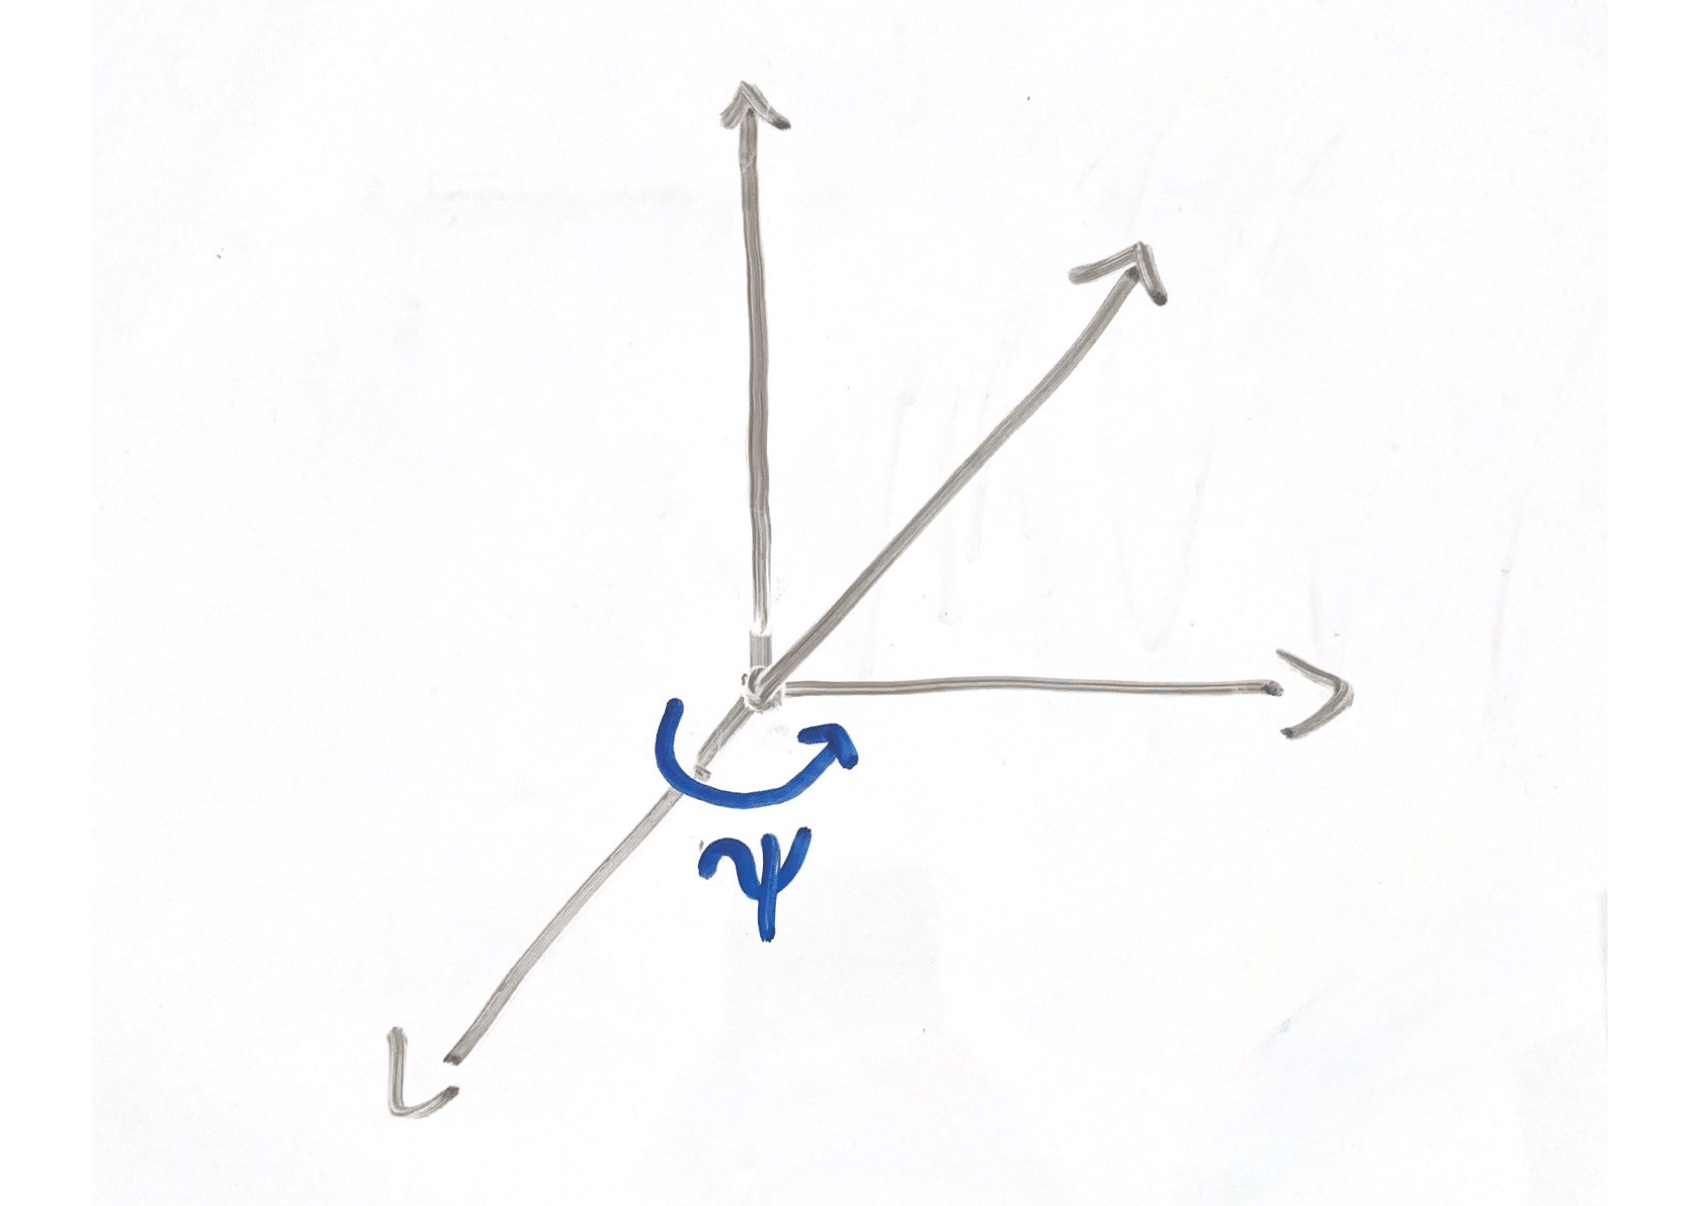
\includegraphics[width=0.4\textwidth]{Rnpsi1.png}
&
		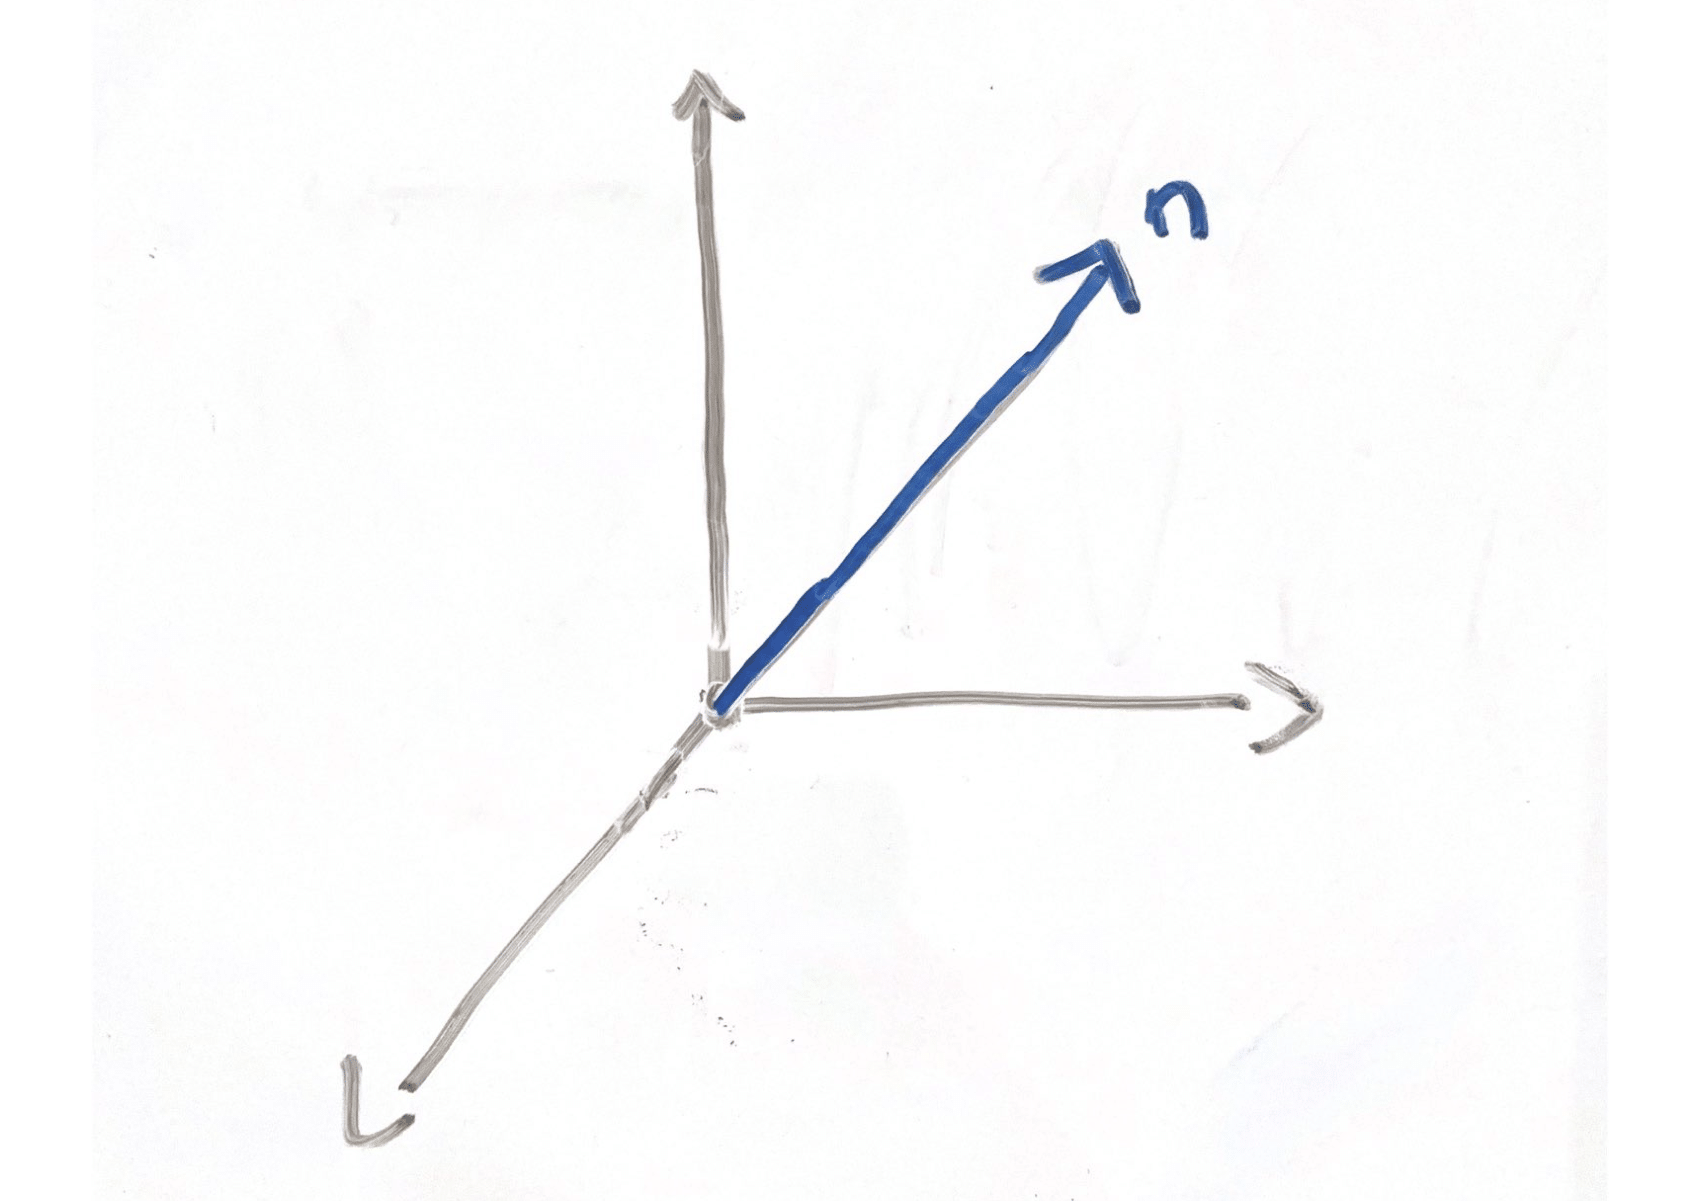
\includegraphics[width=0.4\textwidth]{Rnpsi2.png}
	\end{tabular}
	\caption{Theorem 3.1: $R_n(\psi)$}
	

\end{figure}
\begin{figure}[H]
	\centering

	\begin{tabular}{ccc}
		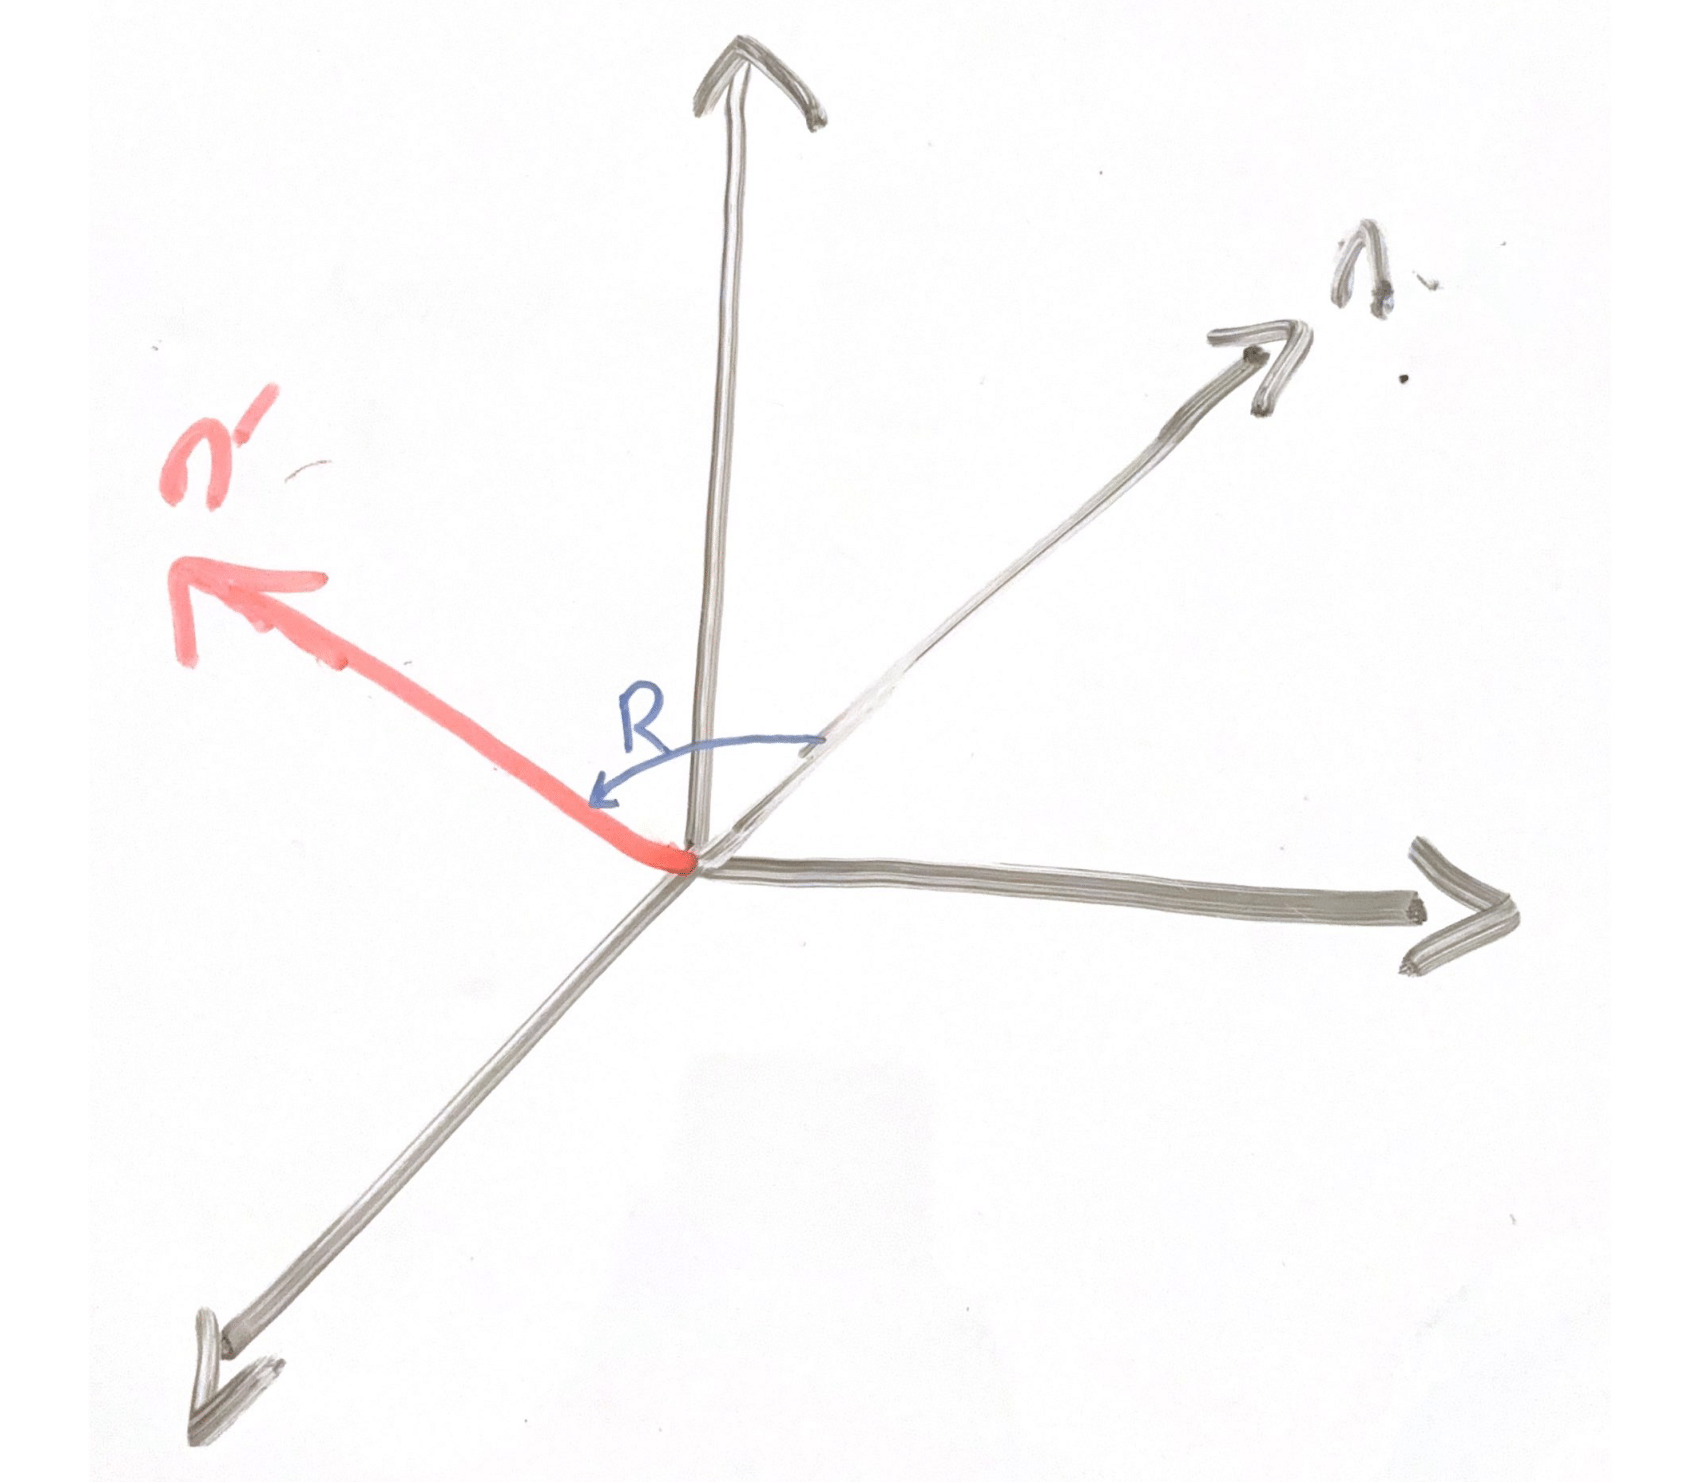
\includegraphics[width=0.3\textwidth]{RRnR1.png}
		&
		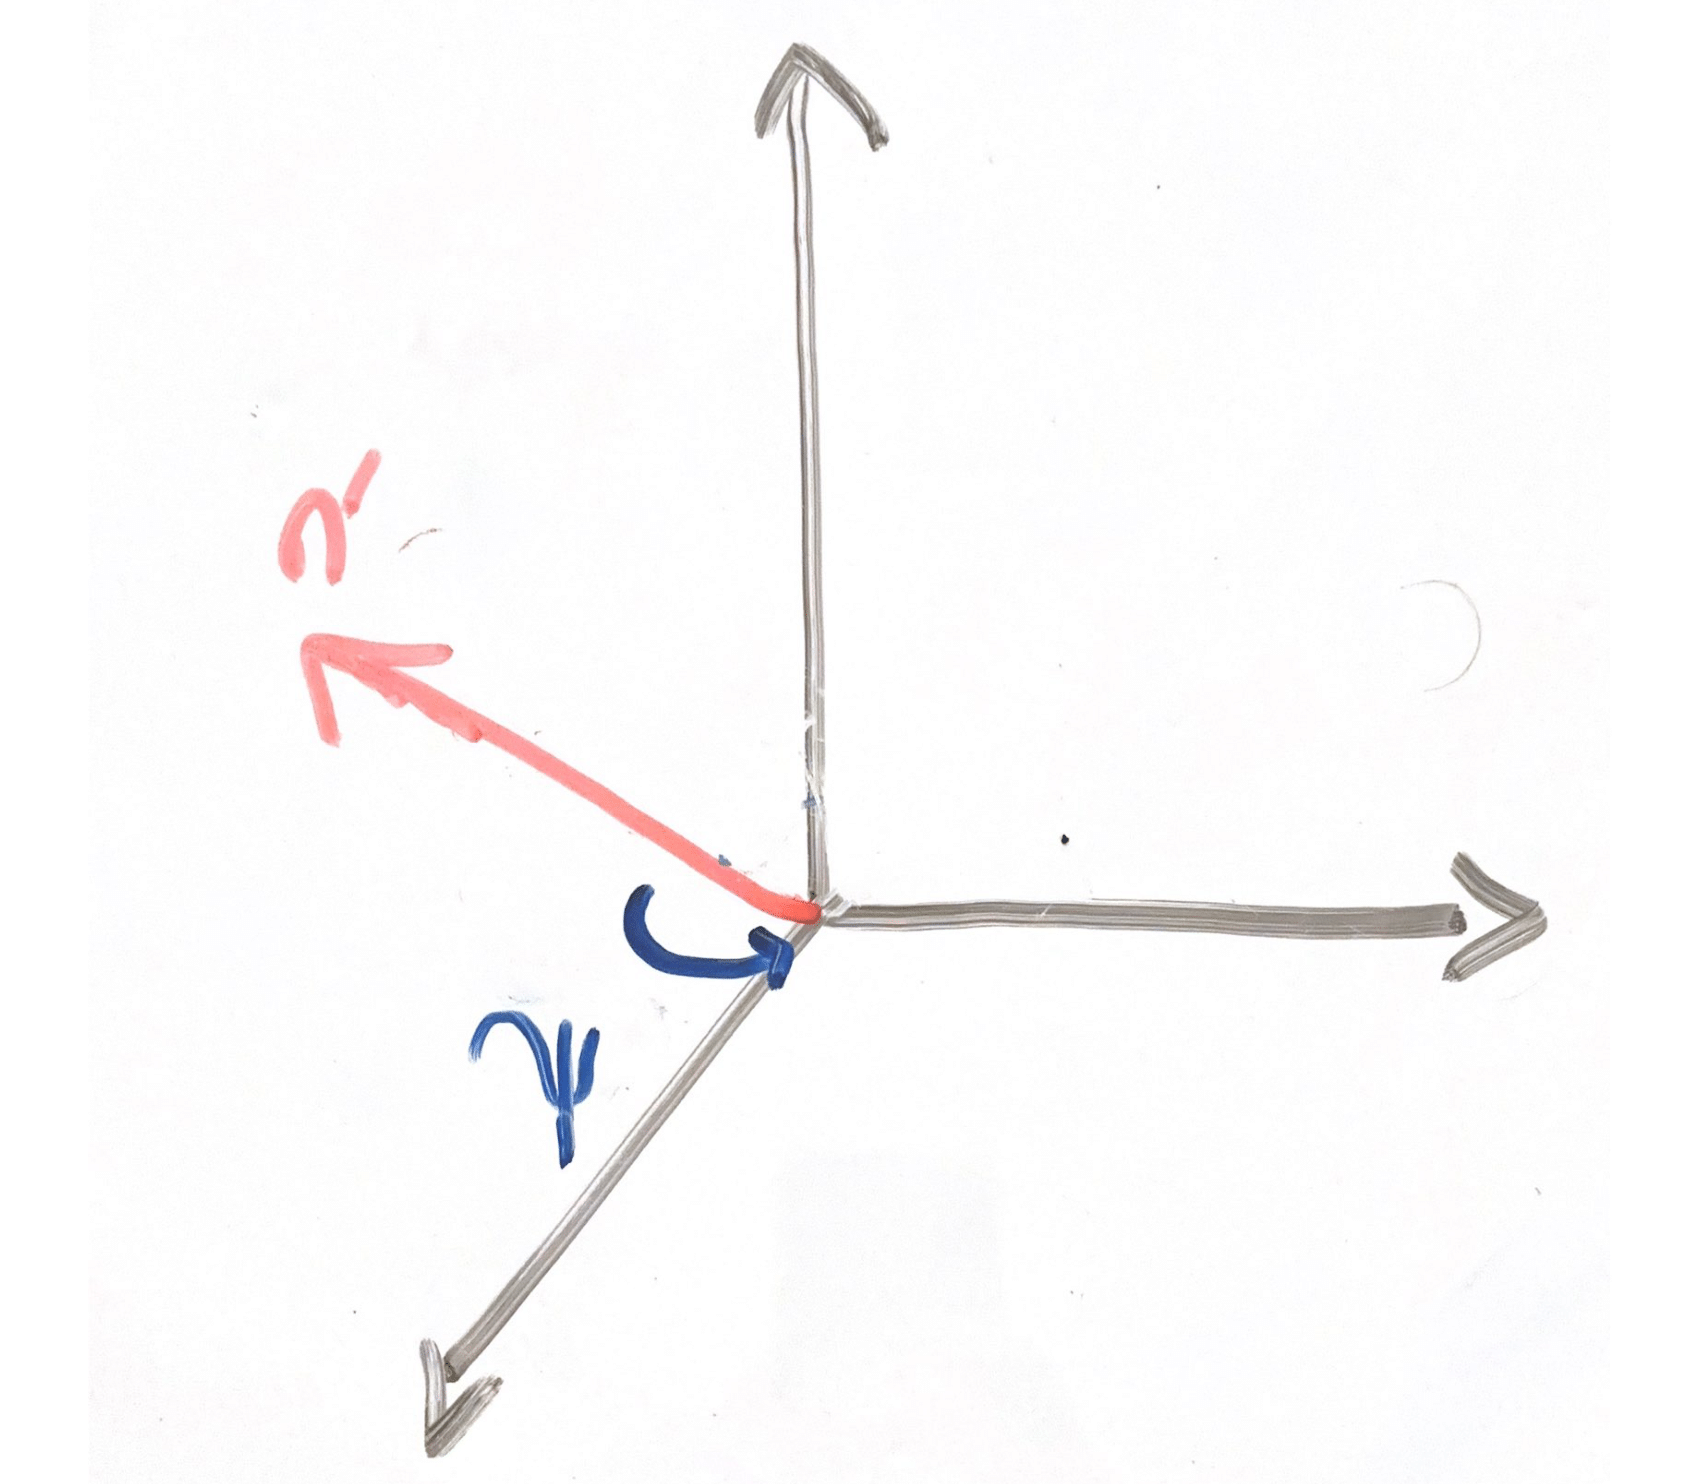
\includegraphics[width=0.3\textwidth]{RRnR2.png}\\
		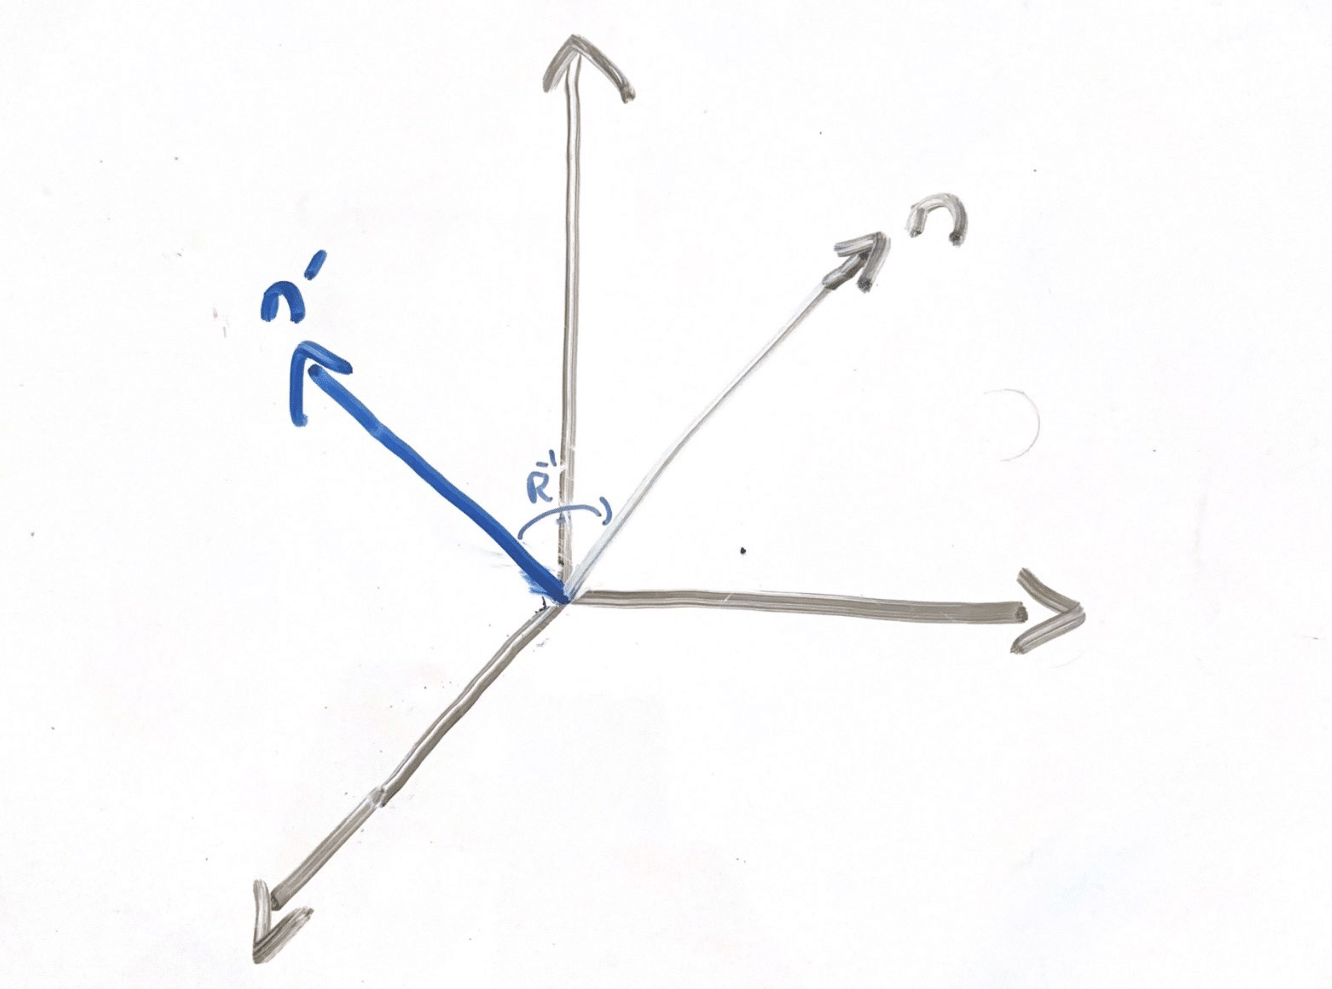
\includegraphics[width=0.3\textwidth]{RRnR3.png}
		&
		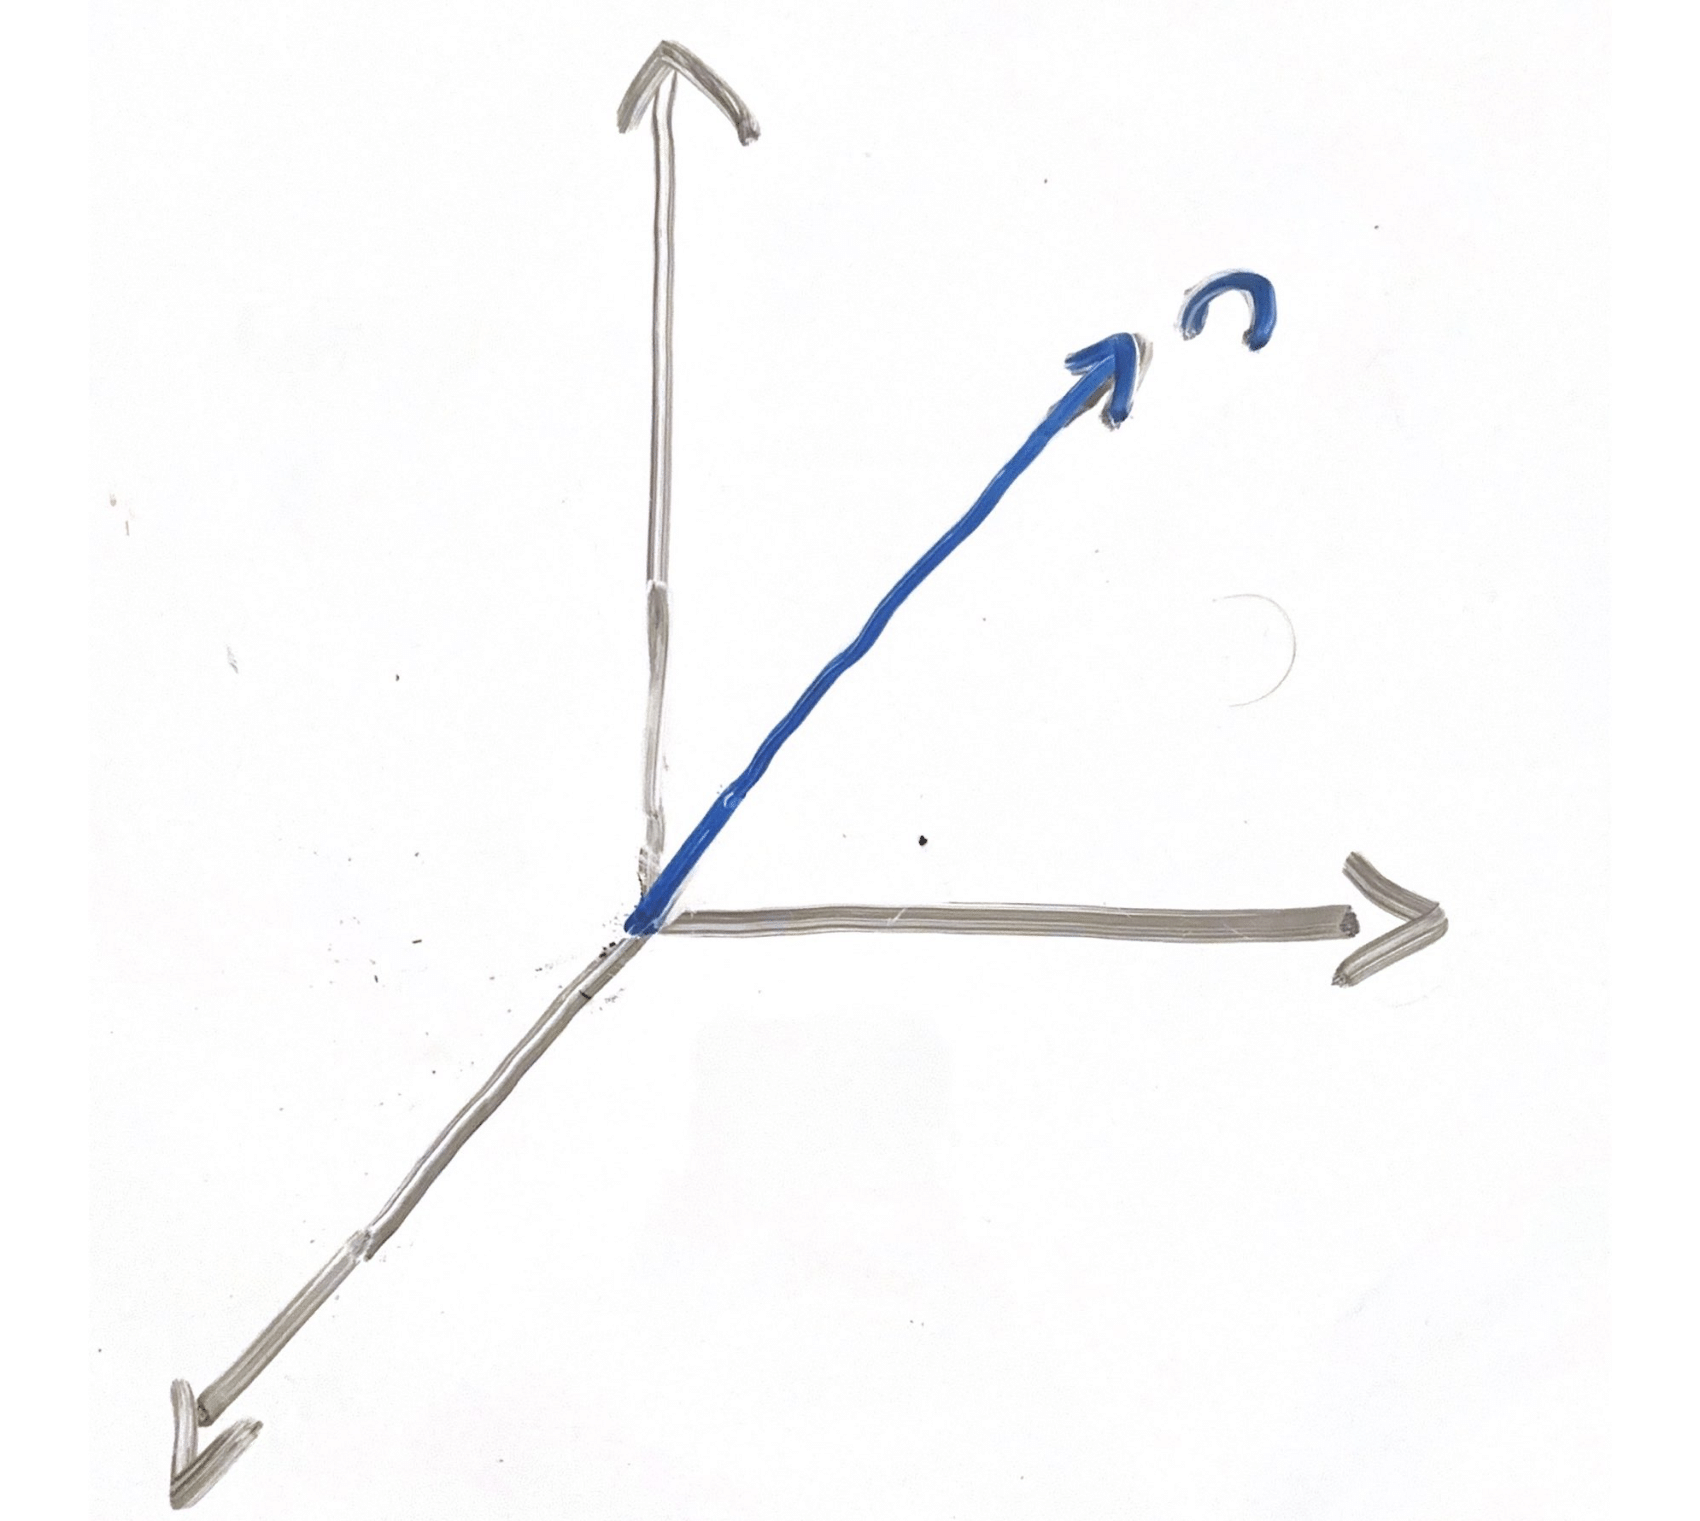
\includegraphics[width=0.3\textwidth]{RRnR4.png}

	\end{tabular}
	\caption{Theorem 3.1: $R^{-1}R_{n'}(\psi)R$}
	

\end{figure}



With this identifty in mind, we can make a deeper conclusion about the inherent structure of $SO(3)$.

\begin{corrolary}
	All rotations (about any axis) by a fixed angle $\psi$ share a conjugacy class (denoted $C_\psi$).
\end{corrolary}

These classifications of rotations give us our first way of understanding rotations in $SO(3)$. There is another equally useful way to interpret any rotation in $\R^3$. Suppose our coordinate axes are defined by the following convention: $(x,y,z)$. A rotation in $SO(3)$ will change the direction that these axes point in, but still will preserve the inherent mutual orthogonality of the directions. We will refer to the initial axes as the "fixed frame" and the rotated axes, $(x',y',z')$, as the rotated frame. The natural question would be to ask how we can characterize the transition from the fixed frame to the rotated frame.

\begin{definition}
	Let $(x,y,z)$ be the fixed frame and let $(x',y',z')$ be any rotated frame. Then this rotation's \textbf{Euler Angles} decompose the rotation in the following way:
$$R(\alpha,\beta,\gamma) \coloneq R_{z'}(\gamma)R_n(\beta)R_z(\alpha)$$
where $n$ points in the direction defined by the intersection of the $xy$ and $x'y'$ planes (or equivalently, the $z\times z'$ direction). Note: we use the subscript $z$ and $z'$ as a shorthand to mean the $z$-axis and $z'$-axis.
\end{definition}

In this way, we view every rotation in $SO(3)$ as the composition of three rotations about mutually orthogonal axes. Conventionally, we restrict the parameters to the followign conditions: $\alpha,\gamma\in[0,2\pi)$, $\beta\in[0,\pi]$. This limits double-counting in a similar manner to the discussion above. The figure below illustrates the use of Euler angles to complete an arbitrary rotation as the composition of three determined rotations.\\

\begin{figure}[H]
	\centering
	\tdplotsetmaincoords{60}{200}
	\tdplotsetrotatedcoords{60}{45}{225}
	\begin{tikzpicture}
			[scale=2,
				tdplot_main_coords,
				axis/.style={->,black,thin},
				vector/.style={-stealth,black,very thick}]
		\draw[axis,color=gray] (0,0,0) -- (1,0,0) node[anchor=south]{$x$};
		\draw[axis,color=gray] (0,0,0) -- (0,1,0) node[anchor=west]{$y$};
		\draw[axis] (0,0,0) -- (0,0,1) node[anchor=east]{$z$};
		\draw[axis,color=blue] (0,0,0) -- (-0.707106781186548,0.707106781186548,0) node[anchor=west]{$z'$}; 
		\tdplotcrossprod(-0.707106781186548,0.707106781186548,0)(0,0,1);
		\draw[axis,color=red] (0,0,0)--(\tdplotresx,\tdplotresy,\tdplotresz) node[anchor=south]{$n$};
		\tdplotdrawarc[->]{(0,0,0)}{1.2}{0}{315}{anchor=north}{$\alpha$};
	\end{tikzpicture}
	\caption{Euler Angles: Rotating Fixed Frame about $z$-axis by $\alpha$}
		
\end{figure}

\begin{figure}[H]
	\centering
	\tdplotsetmaincoords{60}{200}
	\tdplotsetrotatedcoords{45}{90}{90}
	\begin{tikzpicture}
			[scale=2,
				tdplot_main_coords,
				axis/.style={->,black,thin},
				vector/.style={-stealth,black,very thick}]
		\draw[axis,color=lightgray] (0,0,0) -- (1,0,0) node[anchor=south]{$x$};
		\draw[axis,color=black] (0,0,0) -- (0.7071,-0.7071,0) node[anchor=north]{$x$};
		\draw[axis,color=lightgray] (0,0,0) -- (0,1,0) node[anchor=west]{$y$};
		\draw[axis,color=black] (0,0,0) -- (0,0,1) node[anchor=east]{$z$};
		\draw[axis,color=blue] (0,0,0) -- (-0.707106781186548,0.707106781186548,0) node[anchor=east]{$z'$};
		\tdplotcrossprod(-0.707106781186548,0.707106781186548,0)(0,0,1);
		\draw[axis,color=wildwatermelon] (0,0,0)--(\tdplotresx,\tdplotresy,\tdplotresz) node[anchor=south]{$y$};
		\tdplotdrawarc[->,color=gray]{(0,0,0)}{1.2}{0}{315}{anchor=south east}{$\alpha$};
		\tdplotdrawarc[<-,tdplot_rotated_coords,color=red]{(0,0,0)}{1.2}{0}{90}{anchor=south west}{$\beta$};
	\end{tikzpicture} 
	\caption{Euler Angles: Rotating Intermediate Frame about new $y$-axis by $\beta$}
\end{figure}

\begin{figure}[H]
	\centering
	\tdplotsetmaincoords{60}{200}
	\tdplotsetrotatedcoords{45}{90}{90}
	\begin{tikzpicture}
			[scale=2,
				tdplot_main_coords,
				axis/.style={->,black,thin},
				vector/.style={-stealth,black,very thick}]
		\draw[axis,color=lightgray] (0,0,0) -- (0.7071,-0.7071,0) node[anchor=north]{$x$};
		\draw[axis,color=black] (0,0,0) -- (0,0,1) node[anchor=south]{$x$};

		\draw[axis,color=cobalt] (0,0,0) -- (-0.707106781186548,0.707106781186548,0) node[anchor=west]{$z'$}; %(-sqrt(2)/2,sqrt(2)/2,0)

		\tdplotcrossprod(-0.707106781186548,0.707106781186548,0)(0,0,1);
		\draw[axis,color=wildwatermelon] (0,0,0)--(\tdplotresx,\tdplotresy,\tdplotresz) node[anchor=south]{$y$};

		\tdplotdrawarc[->,color=lightgray]{(0,0,0)}{1.2}{0}{315}{anchor=south east}{$\alpha$};
		\tdplotdrawarc[<-,tdplot_rotated_coords,color=classicrose]{(0,0,0)}{1.2}{0}{90}{anchor=south west}{$\beta$};
		\tdplotsetrotatedcoords{135}{90}{180}
		\tdplotdrawarc[->,tdplot_rotated_coords,color=cobalt]{(0,0,0)}{1.2}{0}{315}{anchor=south}{$\gamma$};
	\end{tikzpicture}
	\caption{Euler Angles: Rotating Intermediate Frame about new $z$-axis by $\gamma$}
\end{figure}

\begin{figure}[H]
	\centering
	\tdplotsetmaincoords{60}{200}
	\tdplotsetrotatedcoords{45}{90}{90}
	
	\begin{tikzpicture}
			[scale=2,
				tdplot_main_coords,
				axis/.style={->,black,thin},
				vector/.style={-stealth,black,very thick}]
		\draw[axis,color=lightgray] (0,0,0) -- (1,0,0) node[anchor=north]{$x$};
		\draw[axis,color=black] (0,0,0) -- (-0.5,-0.5,0.70711) node[anchor=south]{$x'$};
		\draw[axis,color=lightgray] (0,0,0) -- (0,1,0) node[anchor=west]{$y$};
		\draw[axis,color=wildwatermelon] (0,0,0) -- (0.5,0.5,0.70711) node[anchor=north east]{$y'$};
		\draw[axis,color=lightgray] (0,0,0) -- (0,0,1) node[anchor=east]{$z$};
		\draw[axis,color=cobalt] (0,0,0) -- (-0.707106781186548,0.707106781186548,0) node[anchor=east]{$z'$}; 
		\tdplotcrossprod(-0.707106781186548,0.707106781186548,0)(0,0,1);
	
	
		\tdplotdrawarc[->,color=lightgray]{(0,0,0)}{1.2}{0}{315}{anchor=north west}{$\alpha$};
		\tdplotdrawarc[<-,tdplot_rotated_coords,color=classicrose]{(0,0,0)}{1.2}{0}{90}{anchor=north west}{$\beta$};
		\tdplotsetrotatedcoords{135}{90}{180}
		\tdplotdrawarc[->,tdplot_rotated_coords,color=columbiablue]{(0,0,0)}{1.2}{0}{315}{anchor=south}{$\gamma$};
	
	\end{tikzpicture}
	\caption{Euler Angles: Rotated Frame}
\end{figure}

\begin{figure}[H]
	\centering
	\tdplotsetmaincoords{60}{200}
	\tdplotsetrotatedcoords{45}{90}{90}
	\begin{tikzpicture}
			[scale=2,
				tdplot_main_coords,
				axis/.style={->,black,thin},
				vector/.style={-stealth,black,very thick}]
		\draw[axis,color=lightgray] (0,0,0) -- (1,0,0) node[anchor=north]{$x$};
		\draw[axis,color=black] (0,0,0) -- (-0.5,-0.5,0.70711) node[anchor=south]{$x'$};
		\draw[axis,color=lightgray] (0,0,0) -- (0,1,0) node[anchor=west]{$y$};
		\draw[axis,color=black] (0,0,0) -- (0.5,0.5,0.70711) node[anchor=north east]{$y'$};
		\draw[axis,color=lightgray] (0,0,0) -- (0,0,1) node[anchor=east]{$z$};
		\draw[axis,color=black] (0,0,0) -- (-0.707106781186548,0.707106781186548,0) node[anchor=east]{$z'$}; 
		\draw[axis,color=red] (0,0,0) -- (0.707106781186548,0.707106781186548,0) node[anchor=south]{$n$}; 
	
		\coordinate (p1) at (1.1,1.1,0);
		\coordinate (p2) at (-1.1,1.1,0);
		\coordinate (p3) at (-1.1,-1.1,0);
		\coordinate (p4) at (1.1,-1.1,0);
		\coordinate (p5) at  (1.1,1.1,1);
		\coordinate (p6) at (1.1,1.1,-1);
		\coordinate (p7) at (-1.1,-1.1,-1);
		\coordinate (p8) at (-1.1,-1.1,1);
	
	
	
		\draw[color=lightgray] (p1) -- (p2);
		\draw[color=lightgray] (p2) -- (p3);
		\draw[color=lightgray] (p3) -- (p4);
		\draw[color=lightgray] (p4) -- (p1);
		\draw[color=black] (p5) -- (p6);
		\draw[color=black] (p6) -- (p7);
		\draw[color=black] (p7) -- (p8);
		\draw[color=black] (p8) -- (p5);
		\draw[dashed,color=red,very thin] (1.1,1.1,0)--(-1.1,-1.1,0);
	
	\end{tikzpicture}

	\caption{Euler Angles: Identifying $n$}

\end{figure} 

An couple important observations can be made by observing these figures: $R_n(\beta)$ is the rotation that moves $z$ to $z'$ and $R_z(\alpha)$ is the rotation that moves $y$ to $n$. Using this fact and Theorem (3.1), we can conclude the following:

\begin{equation}
	\begin{aligned}
		R_{z'}(\gamma) = R_n(\beta)R_z(\gamma)R_n(\beta)^{-1}
	\end{aligned}
\end{equation}
\begin{equation}
	\begin{aligned}
		R_n(\beta) = R_z(\alpha)R_y(\beta)R_z(\alpha)^{-1}
	\end{aligned}
\end{equation}
\begin{equation}
	\begin{aligned}
		R(\alpha,\beta,\gamma) = R_z(\alpha)R_y(\beta)R_z(\gamma)
	\end{aligned}
\end{equation}
where (3.3) comes from applying (3.1-2) to Definition (3.3). This result tells us that every rotation can be categorized three angles we use to rotate about the $y$ and $z$ axis. While any orthogonal basis can serve as our fixed frame, we get the most use out of choosing the standard basis. In doing so, we focus our attention to $xy$-plane and the $xz$-planes when rotating about the $z$ and $y$ axes respectively. In these two-dimensional settings, we can construct $SO(2)$-like matrices that impact the right coordinates of vectors in $\R^3$. To this end, we see that

\begin{equation}
	\begin{aligned}
		R_z(\theta) = \begin{bmatrix}
						\cos(\theta) & -\sin(\theta) & 0 \\
						\sin(\theta) & \cos(\theta) & 0 \\
						0 & 0 & 1 \\
						\end{bmatrix}
	\end{aligned}
\end{equation}

\begin{equation}
	\begin{aligned}
		R_y(\theta) = \begin{bmatrix}
						\cos(\theta) & 0& \sin(\theta) \\
						0 & 1 & 0 \\
						-\sin(\theta) &0& \cos(\theta) \\
						\end{bmatrix}
	\end{aligned}
\end{equation}

\begin{equation}
	\begin{aligned}
		R_x(\theta) = \begin{bmatrix}
						1 & 0 & 0 \\
						0 & \cos(\theta) & -\sin(\theta) \\
						0 & \sin(\theta) & \cos(\theta) \\
						\end{bmatrix}
	\end{aligned}
\end{equation}

and therefore, any rotation in $SO(3)$ can be written as


\begin{equation}
	\begin{aligned}
		R(\alpha,\beta,\gamma) \\&= \begin{bmatrix}
						\cos(\alpha)\cos(\beta)\cos(\gamma) - \sin(\alpha)\sin(\gamma)& -\cos(\alpha)\cos(\beta)\sin(\gamma) -\sin(\alpha)\cos(\gamma)&  \cos(\alpha)\sin(\beta)\\
						\sin(\alpha)\cos(\beta)\cos(\gamma) + \cos(\alpha)\sin(\gamma)& -\sin(\alpha)\cos(\beta)\sin(\gamma) +\cos(\alpha)\cos(\gamma)  &  \sin(\alpha)\sin(\beta) \\
						-\sin(\beta)\cos(\gamma) & \sin(\beta)\sin(\gamma) & \cos(\beta)\\
						\end{bmatrix}
	\end{aligned}
\end{equation}

While this formulation is unpleasing, it is still useful, especially in context of writing computer algorithm.

Now that we have discussed the general form of a matrix in $SO(3)$, we can explore the concept of generators for this group. We can begin by observing that whenever we fix an axis, $n$, that we rotate about, the rotations of all angles about $n$ form a subgroup, call it $H_n$. The argument for this is as follows: Clockwise rotations about $n$ are inverses of counter-clockwise rotations about $n$ and consecutive rotations about the same axis can be done in one rotations if we first add up the angle measures. The matrices of $SO(3)$ must respect these properties or the group does not represent the physical phenomenon of rotation. This being said, we can see that fixing the axis $n$ forces all rotations to take place in the two dimensional plane normal to $n$. For this reason, we can argue that any subgroup constructed in this way must be isomorphic to $SO(2)$, taking the following map:

$$\phi:H_n \rightarrow SO(2)$$
$$R_n(\theta) \mapsto R(\theta)$$

Given this isomorphic relationship, we can construct a generator for $H_n$ in a very similar way that we did to $SO(2)$. If we derive the generator $J_n$ for each $H_n$, we will see the following must be true:

\begin{equation}
	\begin{aligned}
		R_n(\theta) = e^{i\theta J_n}
	\end{aligned}
\end{equation}

\begin{equation}
	\begin{aligned}
		J_x &= \begin{bmatrix}
					0 & 0 & 0 \\
					0 & 0 & -i \\
					0 & i & 0
					\end{bmatrix}
	\end{aligned}
\end{equation}
\begin{equation}
	\begin{aligned}
		J_y &= \begin{bmatrix}
					0 & 0 & i \\
					0 & 0 & 0 \\
					-i & 0 & 0
					\end{bmatrix}
	\end{aligned}
\end{equation}
\begin{equation}
	\begin{aligned}
		J_z &= \begin{bmatrix}
					0 & -i & 0 \\
					i & 0 & 0 \\
					0 & 0 & 0
					\end{bmatrix}
	\end{aligned}
\end{equation}


\begin{theorem}
	 For any arbitrary direction, $n=(n_1,n_2,n_3)\in\R^3$, the generator, $J_n$, of $H_n$, can be written in the following way:
$$J_n = n_1J_x + n_2J_y + n_3J_z$$
\end{theorem}
\noindent \begin{proof}[\cite{Tung}] If $n$ is determined by the prototypical angles $\phi$ and $\theta$, then we can always rotate the $z$-axis into $n$ with the rotation $R(\theta,\phi,0)$. Therefore, $n_i = [R(\theta,\phi,0)]_{i3}$.

\begin{figure}[H]
	\centering
	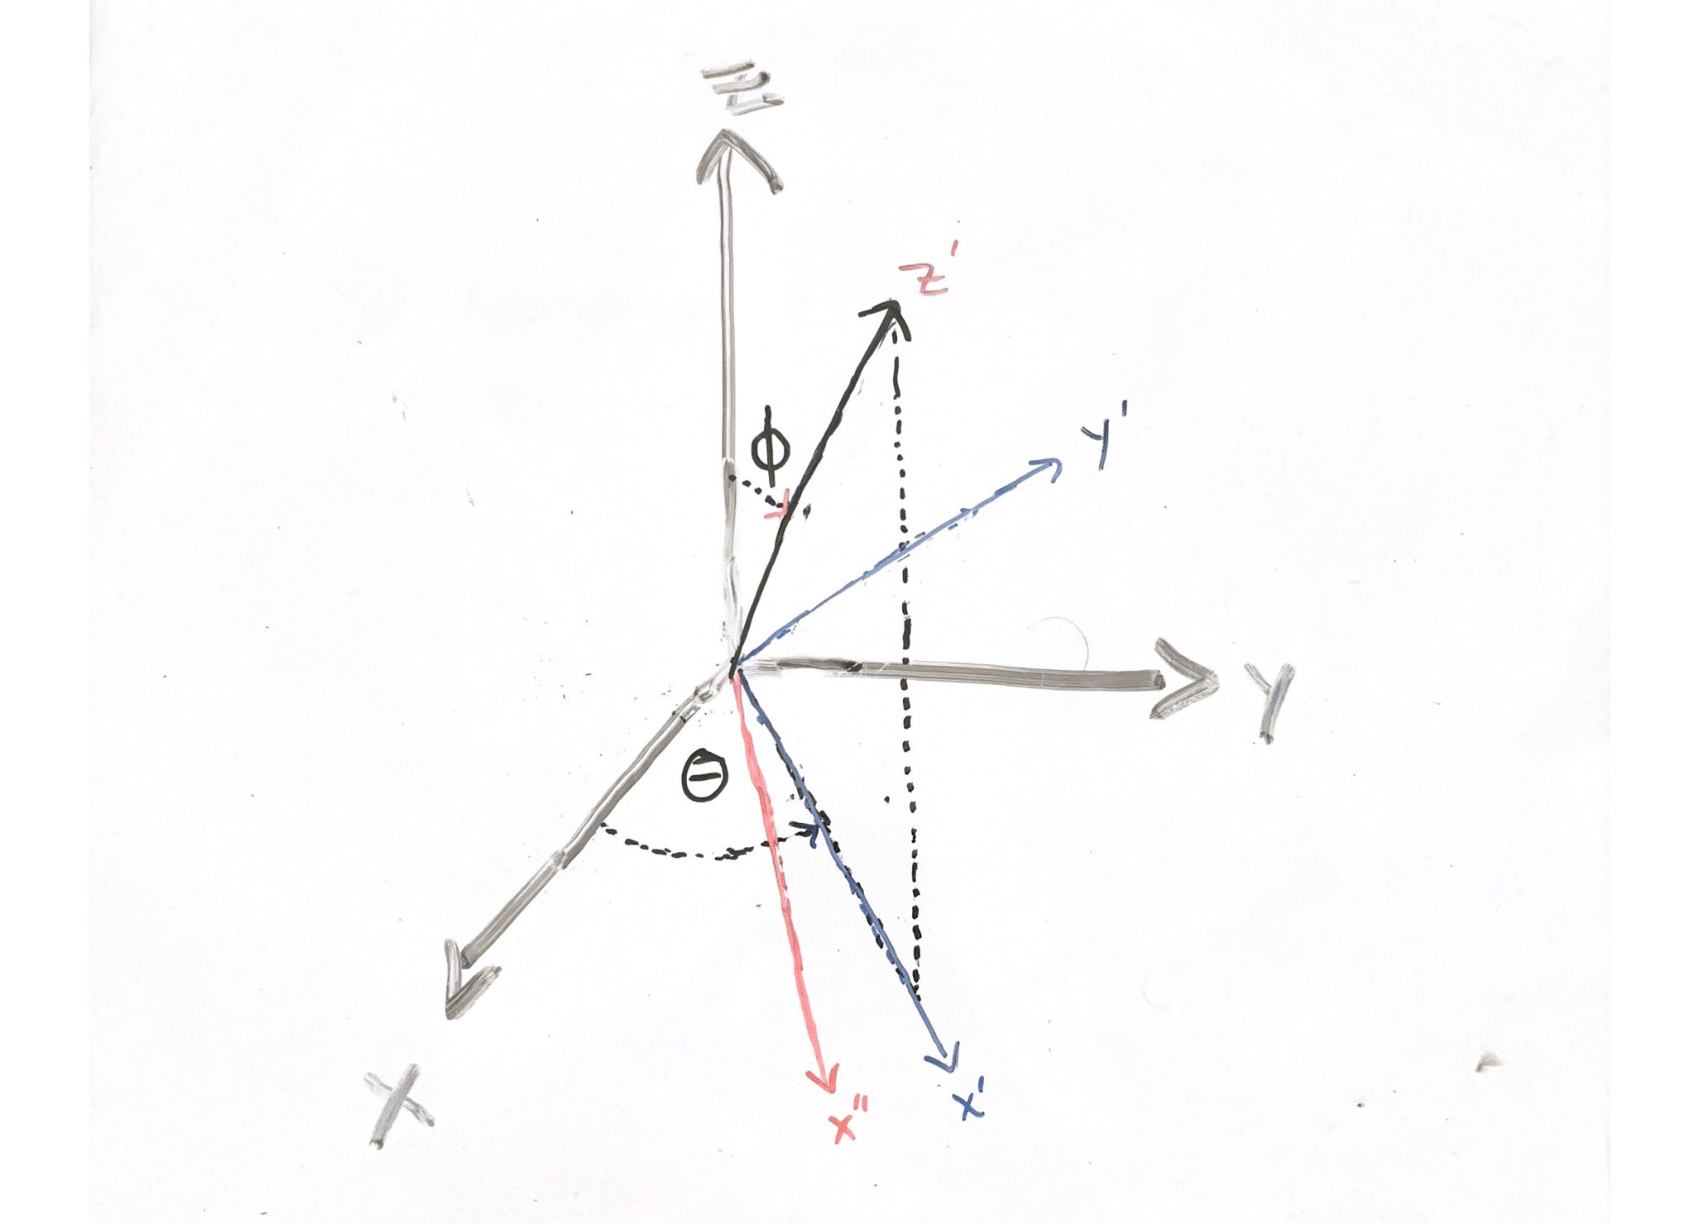
\includegraphics[width=0.7\textwidth]{pushzton}
	\caption{Rotation of the $z$-axis onto $n$}
\end{figure}

Using (3.8) and the above matrix, we can establish a relationship between $J_z$ and $J_n$. For any angle of rotation, $\psi$,

\begin{equation}
	\begin{aligned}
		e^{i\psi J_n} \\
							&= R_n(\psi)	\\
							&=R(\theta,\phi,0)R_z(\psi)R(\theta,\phi,0)^{-1}\\
							&=R(\theta,\phi,0) e^{i\psi J_z} R(\theta,\phi,0)^{-1}\\ 
							&= R(\theta,\phi,0) \sum_{n=0}^\infty \frac{(i\psi J_z)^n}{n!} R(\theta,\phi,0)^{-1} \\
							&= \sum_{n=0}^\infty \frac{(i\psi R(\theta,\phi,0)J_zR(\theta,\phi,0)^{-1})^n}{n!} \\
							&= e^{i\psi R(\theta,\phi,0)J_z R(\theta,\phi,0)^{-1}}\\
	\end{aligned}
\end{equation}

Comparing both sides of the equation, we can see that 

\begin{equation}
	\begin{aligned}
		J_n = R(\theta,\phi,0)J_z R(\theta,\phi,0)^{-1}
	\end{aligned}
\end{equation}

Further, arduous matrix algebra can be done explicitly to show the following identity holds: For any rotation matrix, $R$, and a specified generator, $J_k\in\{J_x,J_y,J_z\}$,

\begin{equation}
	\begin{aligned}
		RJ_kR^{-1} = J_x [R]_{1k} + J_y  [R]_{2k}  +J_z  [R]_{3k} 
	\end{aligned}
\end{equation}

Showing this is true consists of proving it for $R_z(\alpha)$ and $R_y(\beta)$ and arguing that any product of matrices of this form will also work. Combining (3.13) and (3.14), we get 

\begin{equation}
	\begin{aligned}
		J_n &= R(\theta,\phi,0)J_z R(\theta,\phi,0)^{-1} \\
			&= J_x * [R(\theta,\phi,0)]_{13} + J_y * [R(\theta,\phi,0)]_{23}  +J_z * [R(\theta,\phi,0)]_{33}\\
			 &= n_1J_x + n_2J_y + n_3J_z 
	\end{aligned}
\end{equation} 
\end{proof}

In this way, we can see that the generator of a rotation about any direction is a linear combination of the generators about our coordinate axes. For any generic rotation, $\psi$, about $n$, we see that 

\begin{equation}
	\begin{aligned}
		R_n(\psi) = e^{-i\psi n_1J_x}e^{-i\psi n_2J_y}e^{-i\psi n_3J_z}
	\end{aligned}
\end{equation} 

We can use this equation to write it in terms of a rotation's Euler angles in the following way:

\begin{equation}
	\begin{aligned}
		R(\alpha,\beta,\gamma) = e^{-i\alpha J_z}e^{-i\beta J_y}e^{-i\gamma J_z}
	\end{aligned}
\end{equation} 

In this sense, rotation in $\R^3$ can be written simply in terms of the angle measures and generators about coordinate axes.

\section{Irreducible Representations of $SO(3)$}

In order to uncover the irreducible representations of $SO(3)$, we will embark upon the same strategy that we used to find irreducible representations of $SO(2)$. Explicitly, we are looking to find invariant subspaces of our generator. However, we now have three generators to check, and the invariant subspace that we find has to coincide with every possible rotation built from the three. To add more complexity to this matter, we no longer are in an abelian group, which makes our struggle greater for a few reasons. First, finding invariant subspaces under these generators will be dependent on the order in which we apply the rotations. Secondly, irreducible representations need not be degree one anymore. We need to find an invariant subspace that exists independent of order of rotation and that works with all our generators that is spanned by possibly an infinite set of vectors.

First, let us tackle the problem of commuting. We begin with the following definition.

\begin{definition}
	The \textbf{commutator} of two matrices $A$ and $B$ is defined by to be 
$$[A,B]=AB-BA$$
\end{definition}

By definition, two operators/matrices commute if and only if their commutator is equal to $0$. With this in mind, we can expect the generators of our rotations to have the following nontrivial commutators.

\begin{theorem}
	Let $J_k,J_l \in \{J_x,J_y,J_z\}$. Consider the word $xyz$, and all 6 rearrangements of it (identifying each rearrangement with a permutation in $S_3$). Then 
$$[J_k , J_l] = \begin{cases}
					0 & \text{if }k = l \\
					isign(klm)J_m& \text{else}
					\end{cases}$$
where $m$ is the label of the remaining generator in $\{J_x,J_y,J_z\}$.
\end{theorem}

\noindent\begin{proof} These nine commutators can all be verified by direct calculation. In the case where $k=l$, $[J_k,J_k] = J_kJ_k - J_kJ_k = 0$. However, if $k\neq l$, the calculation is dependent on the choice for $k$ and $l$. We will illustrate one example, and the other five commutators can be verified to follow a similar pattern. Take $k=x$ and $l=y$, our word $klm=xyz$ which represents the trivial permutation. Therefore, $sign(xyz)=1$.

\begin{equation}
	\begin{aligned}
		[J_x,J_y] &= J_xJ_y - J_yJ_x \\
					&= \begin{bmatrix}
							0 & 0 & 0\\
							0 & 0 & -i\\
							0 & i & 0
						\end{bmatrix}
						 \begin{bmatrix}
							0 & 0 & i\\
							0 & 0 & 0\\
							-i & 0 & 0
						\end{bmatrix}
						-
						\begin{bmatrix}
							0 & 0 & i\\
							0 & 0 & 0\\
							-i & 0 & 0
						\end{bmatrix}
						 \begin{bmatrix}
							0 & 0 & 0\\
							0 & 0 & -i\\
							0 & i & 0
						\end{bmatrix}\\
					&=  \begin{bmatrix}
							0 & 0 & 0\\
							-1 & 0 & 0\\
							0 & 0 & 0
						\end{bmatrix}
						-
						 \begin{bmatrix}
							0 & -1 & 0\\
							0 & 0 & 0\\
							0 & 0 & 0
						\end{bmatrix} \\
					&= \begin{bmatrix}
							0 & 1 & 0\\
							-1 & 0 & 0\\
							0 & 0 & 0
						\end{bmatrix} \\
					&=i \begin{bmatrix}
							0 & -i & 0\\
							i & 0 & 0\\
							0 & 0 & 0
						\end{bmatrix} \\
					&= i*sign(xyz)*J_z\\
	\end{aligned}
\end{equation} 

Clearly, transposing $x$ and $y$ will make the commutator negative (applying a transposition to $x$ and $y$ turns the word into $yxz$, so this is kept track of in the sign term). The other four cases can be recovered in a symmetric way. \end{proof}

While we can clearly see that these relationships give us a non-commutative structue, we can still glean some value from these these commutators if we use them in a different context.

\begin{definition}
	A \textbf{Lie Algebra} is a vector space, $\mathfrak{g}$, together with a bilinear operation, $[\dot,\dot]$ that satisfies the the following identities:
\begin{itemize}
	\item$ [x,x] = 0$  $\forall x\in\mathfrak{g}$
	\item $[x,[y,z]] + [y,[z,x]] + [z[y,x]]= 0 $ $\forall x,y,z\in\mathfrak{g}$
\end{itemize}
\end{definition}

If we consider the commutator operation our bilinear operation, we can construct create a Lie algebra (using standard addition and scalar multiplication of matrices). Keeping the generators $\{J_x,J_y,J_z\}$, we will denote this Lie algebra as $\mathfrak{so}(3) := \{a_1J_x + a_2J_y + a_3Jz \mid a_1,a_2,a_3\in\C\}$ We can see than any arbitrary element, $M\in \mathfrak{so}(3)$ takes the following form:

\begin{equation}
	\begin{aligned}
		M=i\begin{bmatrix}
		0 & -a_3 & a_2 \\
		 a_3 & 0 & -a_1\\
		-a_2 & a_1 & 0
		\end{bmatrix}
	\end{aligned}
\end{equation} 

showing us that there is a one-to-one correspondence between the skew-symmetric matrices of size $3\times 3$ and matrices in $\mathfrak{so}(3)$. With this in mind, we can make the arguement that any representation of this Lie algebra ($\mathfrak{so}(3)$) will provide use with a representation of the Lie group ($SO(3)$). There is a deep reason for this connection that can be explored in the following source \cite{Hall}. The process for this is much the same as embarked upon for $SO(2)$, but since those representations were one-dimensional and revolved only around one generator, it was not necessary to introduce the complexity of Lie algebras just yet to create the representations. 

As we search for the representations of $\mathfrak{so}(3)$, we still need to find commuting generators. For the moment, it seems that we did not reduce our problem whatosever, but rather added a layer of abstraction. In light of this, we can add even more abstraction to eventually shed some clarity on our circumstances.

\begin{definition}
	The \textbf{universal enveloping algebra} of a Lie algebra is the largest embedding of Lie algebra into an algebra. 
\end{definition}

The inherent utility of the universal enveloping algebra (of a Lie algebra) is that it is the most generic algebra that perserves the commutating properties of the Lie algebra. We will later discuss the necessity of appealing to this larger structure, but we will discuss what this space actuall looks like. 

The construction of the universal enveloping algebra of $\mathfrak{so}(3)$ (which we will denote $A_{\mathfrak{so}(3)}$) follows this prototypical scheme: First, we construct the tensor algebra of $\mathfrak{so}(3)$. This takes the following form:

\begin{equation}
	\begin{aligned}
		T(\mathfrak{so}(3)) = \bigoplus_{i=0}^\infty \left(\bigotimes_{k=0}^i \mathfrak{so}(3)\right) = \left(\C\right) \oplus \left(\mathfrak{so}(3)\right) \oplus \left(\mathfrak{so}(3)\otimes \mathfrak{so}(3)\right) \oplus \hdots
	\end{aligned}
\end{equation} 

Now that we have created (free) tensor algebra on elements of $\mathfrak{so}(3)$, we can establish the commutation relations on elements. We identify each of our generators $J_i$ with its counterpart in the tensor algebra, $\mathfrak{J}_i$. We can construct an ideal, $I$ to be generated by the three elements defined below: 

$$\mathfrak{g_i} \coloneq \mathfrak{J}_k \otimes \mathfrak{J}_l - \mathfrak{J}_l\otimes \mathfrak{J}_k - \begin{cases}
	0 & \text{if }k=l	\\
	i*sign(klm) \mathfrak{J}_m &\text{else}
\end{cases}$$

We then gather our universal enveloping algebra on $\mathfrak{so}(3)$ by taking the corresponding quotient space.

$$A_{\mathfrak{so}(3)} \coloneq T(\mathfrak{so}(3)) / I$$

As of now, we have shifted out problem to looking for commutative elements in $A_{\mathfrak{so}(3)}$. What is the inherent significance of this? If we view our generators $J_x$, $J_y$, $J_z$ as elements in $A_{\mathfrak{so}(3)}$, we can see that the commutator relations are still satisfied as they are in $\mathfrak{so}(3)$. However, due to the construction, there is no way to meaningfully combine them. All that we know is that any formal combination of our generators of can potentially be simplified with our commutator relations, and no other information is given. So, we must set out to find an element in $A_{\mathfrak{so}(3)}$ that commutes with all other elements.

\begin{definition}
	A \textbf{Casimir element} of a Lie algebra, $A$, is any element in the center of the universal enveloping algebra of $A$.
\end{definition}

This process, while a seemingly daunting task, is easily solved by taking a well-known physics concept to do the work for us. We define the element $\mathfrak{J^2} \coloneq (\mathfrak{J}_x \otimes \mathfrak{J}_x) \oplus (\mathfrak{J}_y \otimes \mathfrak{J}_y) \oplus (\mathfrak{J}_z \otimes \mathfrak{J}_z) = \mathfrak{J}_x^2 + \mathfrak{J}_y^2 + \mathfrak{J}_z^2$ where we suppress the tensor algebra notation for easier readbility. (It can be intuitively understood that any element referenced in $\mathfrak{this}$ $\mathfrak{script}$ will be contained in $A_{\mathfrak{so}(3)}$ and abide by its properties of multiplication).

\begin{theorem}
	$\mathfrak{J^2}$ is a Casimir element.
\end{theorem}

\noindent \begin{proof} Let $k\in \{x,y,z\}$.
\begin{equation}
\begin{aligned}
	[\mathfrak{J^2}, \mathfrak{J}_k] &= [\mathfrak{J}_x^2, \mathfrak{J}_k] + [\mathfrak{J}_y^2, \mathfrak{J}_k] + [\mathfrak{J}_z^2, \mathfrak{J}_k]\\
										 &=\sum_{\substack{m\in\{x,y,z\} \\ m\neq k}} \mathfrak{J}_m [\mathfrak{J}_m, \mathfrak{J}_k] + [\mathfrak{J}_m, \mathfrak{J}_k]\mathfrak{J}_m\\
										&= \mathfrak{J}_{m_1}(i\mathfrak{J}_{l_1})+ (i\mathfrak{J}_{l_1}) \mathfrak{J}_{m_1} + \mathfrak{J}_{m_2}(-i\mathfrak{J}_{l_2}) +(-i\mathfrak{J}_{l_2}) \mathfrak{J}_{m_2} \\
										&= 0
\end{aligned}
\end{equation}
where the last equality is established by the fact that our choice is limited to $m_2$ and $l_2$ are forced to be exactly $l_1$ and $m_1$ respectively. \end{proof}

The natural question to ask is why did we have to build the structure of the universal enveloping algebra to be able to use a seemingly straightforward element. The answer comes from the fact that there is no corresponding $J^2$ element in the Lie algebra $\mathfrak{so}(3)$. A direct computation would show us that:

\begin{equation} 
	\begin{aligned}
		J^2  &= J_x^2 + J_y^2 + J_z^2 \\
					&= \begin{bmatrix}
								0& 0 & 0 \\
								0 & 0 & -i \\
								0 & i & 0
							\end{bmatrix}^2 +\begin{bmatrix}
													0 & 0 & i \\
													0 & 0 & 0 \\
													-i & 0 & 0
												\end{bmatrix}^2 + \begin{bmatrix}
																			0 & -i & 0\\
																			i & 0 & 0 \\
																			0 & 0 & 0
																		\end{bmatrix}^2 \\
					&= \begin{bmatrix}
								0& 0 & 0 \\
								0 & 1 & 0 \\
								0 & 0 & 1
							\end{bmatrix} +\begin{bmatrix}
													1 & 0 & 0 \\
													0 & 0 & 0 \\
													0 & 0 & 1
												\end{bmatrix} + \begin{bmatrix}
																			1 & 0 & 0\\
																			0 & 1 & 0 \\
																			0 & 0 & 0
																		\end{bmatrix} \\
					&= \begin{bmatrix}
								2& 0 & 0 \\
								0 & 2 & 0 \\
								0 & 0 & 2
							\end{bmatrix} \\
					&= 2I_3 \notin \mathfrak{so}(3)
	\end{aligned}
\end{equation} 

Therefore, our discussion must be specific to $A_{\mathfrak{so}(3)}$ in order for us to develop any useful insight with commutative elements.

Letting $\phi$ be any irreducible representation of $A_{\mathfrak{so}(3)}$, the commutativity of $\mathfrak{J^2}$ shows us that for any $\mathfrak{J}_n \in A_{\mathfrak{so}(3)}$, $\phi(\mathfrak{J}_n)\phi(\mathfrak{J^2}) = \phi(\mathfrak{J^2})\phi(\mathfrak{J}_n)$. Schur's Theorem asserts that $\phi(\mathfrak{J^2}) = \lambda I_m$ where $\lambda\in\C$ and $m$ is the degree of the representation. This means that for any $v\in V$ (on which the representations are defined to be operators), $v$ is an eigenvector of $\phi(\mathfrak{J^2})$ with eigenvalue $\lambda$.

In search of our invariant subspace, we now must choose an eigenbasis of $V$ with respect to a basis of commuting generators (whose span collects all possible generators in $A_{\mathfrak{so}(3)}$). We can easily select $\mathfrak{J^2}$ and an additional generator from our typical collection $\{\mathfrak{J}_x,\mathfrak{J}_y,\mathfrak{J}_z\}$, but after choosing one, we can't choose any of the remaining options for fear of not commuting. Conventionally, we select $\{\mathfrak{J^2},\mathfrak{J}_z\}$ as our generators, and choose an eigenbasis of $V$ to be defined with respect to both these generators. With the remaining two generators, we construct two useful linear combinations that will aid us in our efforts.

\begin{equation}
	\begin{aligned}
		\mathfrak{J}_\pm = \mathfrak{J}_x \pm i\mathfrak{J}_y
	\end{aligned}
\end{equation} 

$\mathfrak{J}_+$ is referred to as the ``raising" generator and $\mathfrak{J}_-$ is referred to as the ``lowering generator". It is straightforward to verify that these new generators have special relationships with our conventionally selected generators as seen below:

\begin{equation}
	\begin{aligned}
		[\mathfrak{J}_z,\mathfrak{J}_+] = \mathfrak{J}_+
	\end{aligned}
\end{equation} 
\begin{equation}
	\begin{aligned}
		[\mathfrak{J}_z,\mathfrak{J}_-] = -\mathfrak{J}_-
	\end{aligned}
\end{equation} 
\begin{equation}
	\begin{aligned}
		[\mathfrak{J}_+,\mathfrak{J}_-] = 2\mathfrak{J}_z
	\end{aligned}
\end{equation} 
\begin{equation}
	\begin{aligned}
		\mathfrak{J}^2 = (\mathfrak{J}_z)^2  -\mathfrak{J}_z +\mathfrak{J}_+\mathfrak{J}_- = (\mathfrak{J}_z)^2 +\mathfrak{J}_z+ \mathfrak{J}_-\mathfrak{J}_+
	\end{aligned}
\end{equation} 
\begin{equation}
	\begin{aligned}
		\phi_{\mathfrak{J}_\pm}^\dag = \phi_{\mathfrak{J}_\mp}
	\end{aligned}
\end{equation} 

Using these identities, one can see that for any eigenvector, $v_m$, corresponding to the generator $J_z$ with eigenvalue $m$, then the following two identities hold:

\begin{equation}
	\begin{aligned}
		\phi_{\mathfrak{J}_z\mathfrak{J}_+}(v_m) &= \phi_{\mathfrak{J}_z\mathfrak{J}_+ (-\mathfrak{J}_+\mathfrak{J}_z + \mathfrak{J}_+\mathfrak{J}_z)}(v_m) \\
					&= \phi_{[\mathfrak{J}_z,\mathfrak{J}_+]}(v_m) + \phi_{\mathfrak{J}_+\mathfrak{J}_z}(v_m) \\
					&= \phi_{\mathfrak{J}_+}(v_m) + \phi_{\mathfrak{J}_+\mathfrak{J}_z}(v_m) \\
					&= \phi_{\mathfrak{J}_+(I + \mathfrak{J}_z)}(v_m) \\					
					&= \phi_{\mathfrak{J}_+}((\phi_{I} + \phi_{\mathfrak{J}_z})(v_m)) \\
					&= \phi_{\mathfrak{J}_+}  ((1+m)v_m) \\
					&= (m + 1)\phi_{J_+}(v_m)
	\end{aligned}
\end{equation} 
\begin{equation}
	\begin{aligned}
		\phi_{\mathfrak{J}_z\mathfrak{J}_-}(v_m) &= \phi_{\mathfrak{J}_z\mathfrak{J}_- (-\mathfrak{J}_-\mathfrak{J}_z + \mathfrak{J}_-\mathfrak{J}_z)}(v_m) \\
&=\phi_{[\mathfrak{J}_z,\mathfrak{J}_- ]}(v_m) + \phi_{\mathfrak{J}_-\mathfrak{J}_z}(v_m)\\
					&= \phi_{-\mathfrak{J}_-}(v_m) + \phi_{\mathfrak{J}_-\mathfrak{J}_z}(v_m)\\
					&= \phi_{\mathfrak{J}_-(-I + \mathfrak{J}_z)}(v_m) \\
					&= \phi_{\mathfrak{J}_-}((\phi_{-I} + \phi_{\mathfrak{J}_z})(v_m)) \\
					&= \phi_{\mathfrak{J}_-} ((-1+m)(v_m) \\
					&= (m - 1)\phi_{\mathfrak{J}_-}(v_m)\\
	\end{aligned}
\end{equation} 

These identities give an explicit reason for the naming convention (the raising generator increases the eigenvalue by $1$ and the lowering generator decreases it by $1$). With this, we conclude that repeated applications of $\phi_{\mathfrak{J}_+}$ or $\phi_{\mathfrak{J}_-}$ give us new eigenvectors of $\phi_{\mathfrak{J}_z}$, corresponding to eigenvalues $m + k$ and $m-l$ where $k$ represents the number of repeated applications of $\phi_{\mathfrak{J}_+}$ and $l$ represents the number of repeated applications of $\phi_{\mathfrak{J}_-}$ respectively. We can only repeat this process a finite number of times, as we are working in a finite dimensional vector space. Let us shift our focus somewhat to consider $k$ to be the maximum number of applications of $\phi_{\mathfrak{J}_+}$ before $\phi_{\mathfrak{J}_+}^{k+1}(v_k) = 0$. Let $\lambda$ be the eigenvalue corresponding to eigenvector $\phi_{\mathfrak{J}_+}^{k}(v_{k-1})$ of the operator $\phi_{\mathfrak{J}_z}$. Then, 

\begin{equation}
	\begin{aligned}
		\phi_{\mathfrak{J^2}}\phi_{\mathfrak{J}_+}^k(v_{k-1}) = \phi_{(\mathfrak{J}_z)^2 +\mathfrak{J}_z+ \mathfrak{J}_-\mathfrak{J}_+}(\phi_{\mathfrak{J}_+}^k(v_{k-1})) = \lambda(\lambda + 1) \phi_{J_+}^kv_{k-1}
	\end{aligned}
\end{equation} 

Since $\phi_{\mathfrak{J^2}}$ is a multiple of the identity, it must be the case that $\lambda(\lambda +1)$ is the only eigenvalue of $\phi_{\mathfrak{J^2}}$. Further, repeated applications of $\phi_{\mathfrak{J}_-}$ will decrease the eigenvalue of $\phi_{\mathfrak{J}_z}$ by $1$ for each application. However, this can only happen a finite number of times before we terminate. Therefore, if $l$ is the last application number of applications before  $\phi_{\mathfrak{J}_-}^{l+1}(v_{l}) = 0$ and $\phi_{J_z}v_l = l$.
\begin{equation}
	\begin{aligned}
		0 &= v_{l}  \phi_{\mathfrak{J}_-}^\dag \phi_{\mathfrak{J}_-} v_{l} \\
		&= v_{l} \phi_{\mathfrak{J}_+}\phi_{\mathfrak{J}_-}v_{l} \\
			&= v_{l}\phi_{\mathfrak{J^2} - (\mathfrak{J}_z)^2 + \mathfrak{J}_z}v_{l} \\
		&= \lambda(\lambda+ 1) - l(l - 1)\\
	\end{aligned}
\end{equation} 

Which implies that $\lambda = -l$. Given that we arrived at eigenvalue $l$ from $\lambda$ by applying the lowering operator an integer number of times, $\lambda - l \in \Z^+ \implies 2\lambda\in\Z^+ \implies \lambda = \frac{n}{2}$ for some $n\in\Z^+.$


\begin{theorem}
	The irreducible representations of the $A_{\mathfrak{so}(3)}$ are characterized by eigenvalues that take on positive integer and positive half-integers. If $\lambda$ is one such eigenvalue, then we can construct our eigenvectors, $\{v_m\}_{m=-\lambda}^\lambda$, corresponding to $\phi_{\mathfrak{J}_z}$ with eigenvalue $m$, using the raising or lowering operators. This gives us a degree $2\lambda +1$ representation characterized by the following relationships:
$$\phi_{\mathfrak{J}^2}(v_m) = \lambda(\lambda+1)v_m$$
$$\phi_{\mathfrak{J}_z}(v_m) =  mv_m$$ 
$$v_{m+1} =  \frac{\phi_{\mathfrak{J}_\pm}(v_m)}{\sqrt{\lambda(\lambda+1) - m(m\pm 1)}}$$
\end{theorem}
\noindent where the normalizing factor comes from a brief calculation similar to the matrix product calculation done in (3.32). Theorem (3.10) gives us a way to calculate an irreducible, unitary representation up to any degree. The unitary aspect comes from the fact that $\{v_m\}$ are normalized and orthogonal by their construction. When we do the calculations, we have constructed our operators (in the image of our representation) and seek to construct an orthonormal basis with respect to these operators. As we have shown, following this form will ensure that we cannot create a nontrivial-invariant subspace, due to the fact that the cyclical nature of our eigenbasis construction. Explicitly, every vector in this basis will be an eigenvector of $\phi_{\mathfrak{J^2}}$, and since this operator commutes with every other, we inheret a set of eigenvectors that will span the entire space.

Given our hard work to establish a representation on $A_{\mathfrak{so}(3)}$, we can immediately conclude that we can construct a representation on $SO(3)$. Any rotation under the image of such an irreducible representation must behave in the following way:

\begin{equation}
\begin{aligned}
	\phi_j(R(\alpha,\beta,\gamma)) &= e^{-i\alpha\phi_{\mathfrak{J}_z}}e^{-i\beta\phi_{\mathfrak{J}_y}}e^{-i\gamma\phi_{\mathfrak{J}_z}}	
\end{aligned}
\end{equation}

We are required to compute explicitly $\phi_{\mathfrak{J}_z}$ and $\phi_{\mathfrak{J}_y}$ to make use of these formulas. The following example will illustrate this process more closely.

\begin{example}\end{example}
	Take $\lambda= \frac{1}{2}$. We expect the degree of our representation to be $2$ and we can immediately conclude that:

\begin{equation}
\begin{aligned}
	\phi_{\mathfrak{J^2}} = \begin{bmatrix}
									\frac{3}{4} & 0 \\
									0 & \frac{3}{4}
								\end{bmatrix}
\end{aligned}
\end{equation}
and 
\begin{equation}
\begin{aligned}
	\phi_{\mathfrak{J}_z} = \begin{bmatrix}
									\frac{1}{2} & 0 \\
									0 & \frac{-1}{2}
								\end{bmatrix}
\end{aligned}
\end{equation}

Using the identities found in (3.24-3.28), we can calculate $\phi_{\mathfrak{J}_\pm}$ as 

\begin{equation}
\begin{aligned}
	\phi_{\mathfrak{J}_+} = \begin{bmatrix}
									0 & 1 \\
									0 & 0
								\end{bmatrix}
\end{aligned}
\end{equation}
\begin{equation}
\begin{aligned}
	\phi_{\mathfrak{J}_-} = \begin{bmatrix}
									0 & 0 \\
									1 & 0
								\end{bmatrix}
\end{aligned}
\end{equation}
We can use these two matrices to solve a system of equations to aquire $\phi_{\mathfrak{J}_y}$ and $\phi_{\mathfrak{J}_x}$.
\begin{equation}
\begin{aligned}
	\phi_{\mathfrak{J}_x} = \begin{bmatrix}
									0 & \frac{1}{2} \\
									\frac{1}{2} & 0
								\end{bmatrix}
\end{aligned}
\end{equation}
\begin{equation}
\begin{aligned}
	\phi_{\mathfrak{J}_y} = \begin{bmatrix}
									0 & \frac{1}{2i} \\
									\frac{-1}{2i} & 0
								\end{bmatrix}
\end{aligned}
\end{equation}

We note that $\phi_{\mathfrak{J}_z}$ and $\phi_{\mathfrak{J}_y}$ are a scalar multiple away from having the desirable property that its square is the identity. Therefore, any rotation under $\phi$ is represented by the matrix

\begin{equation}
\begin{aligned}
	&\phi_\frac{1}{2}(R(\alpha,\beta,\gamma)) \\
	&= e^{-i\alpha\phi_{\mathfrak{J}_z}}e^{-i\beta\phi_{\mathfrak{J}_y}}e^{-i\gamma\phi_{\mathfrak{J}_z}}	\\
	&= (\cos(\frac{\alpha}{2})I_2 -i\sin(\frac{\alpha}{2})2*\phi_{\mathfrak{J}_z})(\cos(\frac{\beta}{2})I_2 -i\sin(\frac{\beta}{2})\phi_{\mathfrak{J}_y})(\cos(\frac{\gamma}{2})I_2 -i\sin(\frac{\gamma}{2})\phi_{\mathfrak{J}_z})\\
	&=\begin{bmatrix}
			\cos(\frac{\alpha}{2}) - i (\sin(\frac{\alpha}{2}) & 0\\
			0 & \cos(\frac{\alpha}{2}) + i (\sin(\frac{\alpha}{2})
		\end{bmatrix}
		\begin{bmatrix}
			\cos(\frac{\beta}{2}) & -\sin(\frac{\beta}{2}) \\
			  \sin(\frac{\beta}{2}) & \cos(\frac{\beta}{2}) 
		\end{bmatrix}
\begin{bmatrix}
			\cos(\frac{\gamma}{2}) - i (\sin(\frac{\gamma}{2}) & 0\\
			0 & \cos(\frac{\gamma}{2}) + i (\sin(\frac{\gamma}{2})
		\end{bmatrix} \\
		&=\begin{bmatrix}
			e^{-i\frac{\alpha}{2}}\cos(\frac{\beta}{2})e^{-i\frac{\gamma}{2}} & -e^{-i\frac{\alpha}{2}}\sin(\frac{\beta}{2})e^{-i\frac{\gamma}{2}} \\
			e^{-i\frac{\alpha}{2}}  \sin(\frac{\beta}{2})e^{-i\frac{\gamma}{2}} & e^{-i\frac{\alpha}{2}}\cos(\frac{\beta}{2}) e^{-i\frac{\gamma}{2}}
		\end{bmatrix}
\end{aligned}
\end{equation}

It is worth noting that this example illustrates a multi-valued representation, seeing as $\phi_\frac{1}{2}(R(0,2\pi,0)) = -I_2$. In general, all of the half integer eigenvalue representations will behave in this way.
\chapter{The Euclidean Group in Two and Three Dimensions}\label{En}

While we have discussed rotations extensively, there are many more physical phenomena that are not a result of this action. More specifically, this section will focus on actions that can be represented by compositions of physical rotations and translations. We call the group that takes combinations of these actions the Euclidean Group (in $n$ dimensional space). For the purposes of our study, we will focus on the two and three dimensional cases. While we have covered much of the group for the rotational component of this group, we will need to handle the addition of translations with care. This chapter follows the structure laid out in Wu-ki Tung's \textit{Group Theory in Physics}. \cite{Tung}

\section{Construction and Properties of $E_2$}

\begin{definition}
	The $n$-dimensional \textbf{Euclidean Group, $E_n$,} is the group of all continuous, isometric, linear transformations on $\R^n$.
\end{definition}

For any transformation of this kind, all vectors, $x\in\R^n$, get mapped to $x'\in\R^n$ in the following way 
$$x' = Rx + b$$
for some fixed $R\in SO(n)$ and $b\in\R^n$. This gives us a natural decomposition of our transformation into a rotation (given by the matrix $R$) and a translation (by a vector, $b$).

In two dimensions, our rotations are characterized by one angle and our translations are characterized by one vector in $\R^2$. Therefore, any element can be reference in $E_2$ by choosing $\theta$ and $b$ respectively. For any $g(\theta,b)\in E_2$, $x\overset{g(\theta,b)}{\mapsto}x'$ by through the following transformation:

$$\begin{bmatrix}x'_1\\x'_2\end{bmatrix} = \begin{bmatrix}
			\cos(\theta) & -\sin(\theta) \\
			\sin(\theta) & \cos(\theta) 
		\end{bmatrix} \begin{bmatrix}x_1\\x_2\end{bmatrix} + \begin{bmatrix}b_1\\b_2\end{bmatrix} $$

One can see that through this lens, the composition of transformations in $E_2$ follows the general rule:

$$g(\theta_2,b_2)g(\theta_1,b_1) = g(\theta_2+\theta_1,R(\theta_2)b_1 + b_2)$$

We can construct an invertible matrix to represent each transformation if we take each vector in $\R^2$ to be embedded in $\R^3$ on the $z=1$ plane.

$$\begin{bmatrix}x'_1\\x'_2 \\ 1\end{bmatrix} = \begin{bmatrix}
			\cos(\theta) & -\sin(\theta) & b_1\\
			\sin(\theta) & \cos(\theta) & b_2 \\
			0&0&1
		\end{bmatrix} \begin{bmatrix}x_1\\x_2\\1\end{bmatrix} $$

\noindent Adopting this convetion, we can easily derive the subgroup of $E_2$ corresponding to pure rotations in terms of the generator who's exists we proved in Chapter 2. 

$$J=\begin{bmatrix}
			0 & -i & 0\\
			i & 0 & 0 \\
			0 & 0 & 0
		\end{bmatrix}$$

Turning our focus to the translations, we can perform a similar derivation. At first, we focus on the one dimensional case. For any one-dimensional translation, $T_b(x)\coloneq x + b$,  we can see that translating by a vector with arbitrarily small magnitutde should result in an arbitrarily small translation. Explicitly,

$$T_{dx} = I -idxP$$

\noindent where we will show $P$ to be the generator of translations in a similar calculation to what we did for the generator of $SO(2)$.

We can write $T_x$ in terms of our generator by utilizing the following two equations:

$$T_{x+dx} = T_x + dx \frac{d}{dx}T_x$$
$$T_{x+dx} = T_{dx}T_x$$

Solving this system gives us the same result as in $SO(2)$:

$$T(x) = e^{-iPx}$$

We can explicitly calculate $P$ by looking at how $T_{dx}$ should interact with it.

$$x + dx = T_{dx}(x) = x -idx  P \Rightarrow P = i$$

Generalizing to two dimensions requires we construct the same scheme twice (treating each component separately). Therefore, we get two generator matrices with respect to each component of the matrix specified to be the location for a component of the translation vector.

$$P_x = \begin{bmatrix}
			0 & 0 & i\\
			0 & 0 & 0 \\
			0 & 0 & 0
		\end{bmatrix}, \hspace{3mm}P_y = \begin{bmatrix}
			0 & 0 & 0\\
			0 & 0 & i \\
			0 & 0 & 0
		\end{bmatrix}$$

The physical properties of translations will allow us to create an abelian subgroup of $E_2$ that is restricted to pure translations. Any translation in this group can be written in terms of the generators in the following way:

$$T_b = g(0,b) = e^{-ib_1P_x}e^{-ib_2P_y}$$

Now that we have dealt with rotations and translations separately, we can begin to consider the two physical actions together. A useful observation we can make to this end deals with the relationship between rotations and translations: For any rotation by angle $\theta$, matrix algebra will show that:

$$R(\theta)P_xR(\theta)^{-1} = [R(\theta)]_{11}P_x +  [R(\theta)]_{21}P_y$$
$$R(\theta)P_yR(\theta)^{-1} = [R(\theta)]_{12}P_x +  [R(\theta)]_{22}P_xy$$

With this in mind, it is not a far jump to conclude that for for any translation, $T_b$,

$$R(\theta)T_bR(\theta)^{-1} = T_{R(\theta)b}$$

This identity will is geometrically intuitive and will prove incredibly useful for calculations later. Most usefully, we can see a natural decomposition form for group elements in $E_2$.

\begin{theorem}
	For any $g(\theta,b)\in E_2$, there is a natural decomposition of the transformation into a pure rotation times a pure translation.
$$g(\theta,b) = g(0,b)g(\theta,0)$$
\end{theorem}

\noindent\begin{proof}[\cite{Tung}]
\begin{equation}
\begin{aligned}
g(\theta,b)R(\theta)^{-1} = g(\theta,b)g(-\theta,0) = g(\theta-\theta,b) = T_b 
\end{aligned}
\end{equation}
\end{proof}

Having discussed ways to generically refer to elements of $E_2$, we can begin to discuss the construction of its irreducible representations.

\section{Irreducible Representations of $E_2$}

Much like we did in the last chapter, we will consider the irreducible representations defined on the Lie algebra of its generators to gain insight into the underlying group. Let us begin by characterizing the Lie algebra. We will refer to this structure as $\mathfrak{e_2}$. Given our generators $J, P_x,P_y$, we can explicitly construct a generic element of the Lie algebra as a linear combination.

$$\mathfrak{e_2} = \left\{i\begin{bmatrix}
								0 & -a & b \\
								a & 0 & c \\
								0 & 0 & 0
							 \end{bmatrix} \mid a,b,c \in \C\right\}$$

Now that we have defined our space rigidly, we will begin analyzing the commutators of our generators. It can be easily shown through matrix algebra that the following commutator relations hold:

\begin{equation}
\begin{aligned}
	[P_x,P_y] = 0
\end{aligned}
\end{equation}
\begin{equation}
\begin{aligned}
	[J,P_x] = iP_y
\end{aligned}
\end{equation}
\begin{equation}
\begin{aligned}
	[J,P_y] = -iP_x
\end{aligned}
\end{equation}

The fact that the generators for translations commute with each other gives us a vantage point to analyze an abelian subgroup of $E_2$. Consider the subgroup of pure translations, $T_2 = \{ T_b \coloneq g(\theta,b)\in E_2 \mid \theta=0\}$. Based on our argument with the commutator of generators, this group is abelian. As a result, the quotient group $E_2/T_2$ is well-defined, and intuitively, it is isomorphic to $SO(2)$. Since irreducible representations on quotient groups are irreducible on whole groups \cite{Mendes}, it is clear that our analysis of $SO(2)$ will immediately show us the following irreducible representations of $E_2$.

$$\phi_m:E_2\rightarrow \C$$
$$g(\theta,b)\mapsto e^{im\theta}$$

Now, if we look to encorporate the other generators, we can follow a similar process to how we constructed irreducible representations in $SO(3)$. We begin my constructing the raising and lowering generators in the following way:

\begin{equation}
\begin{aligned}
	P_\pm \coloneq P_x \pm iP_y
\end{aligned}
\end{equation}

 Then, matrix algebra will show that the new commutators on the generators follow the following equality:

\begin{equation}
\begin{aligned}
	[J,P_\pm] = \pm P_\pm 
\end{aligned}
\end{equation}

As we did in the previous chapter, we have to leave the comfort of the Lie algebra and journey into the universal enveloping algebra to find mutually commuting generators. We will denote the universal enveloping algebra of $E_2$ as $A_{\mathfrak{e_2}}$. All of the commutator identities we stated above will clearly translate to identical relations in our new space. As a reminder, when we discuss generators in this space, we will refer to them with our $\mathfrak{special}$ $\mathfrak{script}$. 

In $A_{\mathfrak{e_2}}$, there is a Casimir element similar to that of $A_{\mathfrak{so}(3)}$. 
\begin{equation}
\begin{aligned}
	\mathfrak{P}^2 = (\mathfrak{P}_x)^2 + (\mathfrak{P}_y)^2 = \mathfrak{P}_+\mathfrak{P}_- = \mathfrak{P}_-\mathfrak{P}_+
\end{aligned}
\end{equation}
\begin{equation}
\begin{aligned}
	[\mathfrak{P}^2,J] =[\mathfrak{P}^2,\mathfrak{P}_\pm]  = 0
\end{aligned}
\end{equation}

As is typical with Casimir elements, its image under any irreducible representation is a multiple of the identity. We will call this multiple $p$. Further, as we have done before, any eigenvector of one map can be used to generate (through its application) an eigenvector of a commuting map. Since $\mathfrak{J}$ is defined in the same way that that it is in $SO(2)$, its image under an irreducible representation has eigenvalues corresponding to the integers. Allowing $\psi$ to be an irreducible representation of $A_\mathfrak{e_2}$, we let $v_m$ be an eigenvector of $\phi_\mathfrak{J}$ corresponding to eigenvalue $m\in\Z$ Then the following equations characterize the irreducible representation:
\begin{equation}
\begin{aligned}
	 \psi(\mathfrak{P}^2)v_m = pv_m
\end{aligned}
\end{equation}
\begin{equation}
\begin{aligned}
	 \psi(\mathfrak{J})v_m = mv_m
\end{aligned}
\end{equation}

We can also see that the raising and lowering generators naturally have the desired effect
\begin{equation}
\begin{aligned}
	 \psi(\mathfrak{J}\mathfrak{P}_+)v_m = (m+1)\mathfrak{P}_+v_m
\end{aligned}
\end{equation}
\begin{equation}
\begin{aligned}
	 \psi(\mathfrak{J}\mathfrak{P}_-)v_m = (m-1)\mathfrak{P}_-v_m
\end{aligned}
\end{equation}

Given the way that $\mathfrak{P}^2$ was defined, we can see that $\psi(\mathfrak{P}^2)$ must be positive-definite. Therefore, its eigenvalues are non-zero. In the case where $p=0$, it corresponds to a pure rotation ($\psi(\mathfrak{P}^2) = 0$ and so translation does not occur). Therefore, this corresponds to the irreducible representation we calculated for the quotient group. 

If $p>0$, we will define the sequence of eigenvectors $\{v_m\}_{m\in\Z}$ to be defined by the following way:

\begin{equation}
\begin{aligned}
	 v_{m+1} \coloneq \frac{i}{p}\psi(\mathfrak{P}_+)v_m
\end{aligned}
\end{equation}

As resulting and equivalent way of defining this sequence would be to use the lowering generator $v_{m-1} \coloneq \frac{-i}{p}\psi(\mathfrak{P}_-)v_m$. We will need to use both constructions to collect every vector. Since there is clearly no restriction on $m$, the vector space is infinite dimensional. As a result, we cannot explicitly write down a matrix for the image of any group element under any representation. However, as we began discussing in Section 1.6, we can make reference to matrix elements of our irreducible representations. 

If we use the eigenbasis $\{v_m\}_{m\in\Z}$, then we can find every matrix element evaluated on our generators using the following formulas:

\begin{equation}
\begin{aligned}
	 \langle \psi(\mathfrak{J})v_m , v_{m'} \rangle = \begin{cases}
																m & \text{if }m' = m\\
																0 & \text{else}
															\end{cases}
\end{aligned}
\end{equation}
\begin{equation}
\begin{aligned}
	 \langle \psi(\mathfrak{P}_\pm)v_m , v_{m'} \rangle = \begin{cases}
																\mp ip & \text{if }m' = m \pm 1\\
																0 & \text{else}	
															\end{cases}
\end{aligned}
\end{equation}

With this in mind, we can fully characterize the matrix elements of the irreducible representations of $E_2$.

\begin{theorem}[\cite{Tung}]
	The faithful, unitary, irreducible representations of $E_2$ are characterized by the following equation defined in terms of matrix elements. If $\psi_p$ is a representation corresponding to a $p>0$, then $[\psi_p(g)]_{mm'}$ corresponds to the matrix element specified by the choice of $v_m$, $v_{m'}$, and $g$. The representations, $\psi_p$ have the following form:
$$[\psi_p(g(\theta,b))]_{mm'} = e^{i(m-m')\phi}J_{m-m'}(pr)e^{-im\theta}$$
where $r$ and $\phi$ are the polar coordinates for the vector $b$.
\end{theorem}
\noindent\begin{proof} For any pure rotation, $R(\theta)$, we can see that

\begin{equation}
\begin{aligned}
 \langle \psi(R(\theta))v_m , v_{m'} \rangle = \begin{cases}
																e^{-im\theta} & \text{if }m' = m\\
																0 & \text{else}
															\end{cases}
\end{aligned}
\end{equation}

For any pure translation (given by the polar coordinates $r$ and $\theta$), we can use the fact that

\begin{equation}
\begin{aligned}
	T_{r,\phi} = R(\phi)^{-1}T_{r,0}R(\phi)
\end{aligned}
\end{equation}

and the fact that $\phi$ is unitary to see that 

\begin{equation}
\begin{aligned}
 \langle \psi(T_{r,\phi})v_m , v_{m'} \rangle = e^{i(m-m')\phi}\langle \psi(T_{r,0})v_m , v_{m'} \rangle
\end{aligned}
\end{equation}

In this way, we reduce our problem to consider pure translations in only the positive $x$ direction corresponding to the generator $\mathfrak{P}_x$. We can see that for any pure translation in this direction in terms of the generator

\begin{equation}
\begin{aligned}
	 T_{r,0} &= e^{-ir\mathfrak{P}_x}\\
			&= e^{-ir\frac{\mathfrak{P}_++\mathfrak{P}_-}{2}} \\
			&= \sum_{k,l} \frac{(-1)^k(iP_+)^k\frac{b}{2}^{k+l}(-iP)^l}{k!l!}
\end{aligned}
\end{equation}

When we evaluate the matrix element of this expression at the indices corresponding to $V_m$ and $v_{m'}$, we see that in order for us to have a nonzero evaluation, the terms the powers of the raising and lower operators, $k$ and $l$, have to related to $m$ and $m'$ through the equation $k-l=m'-m$. Holding $k-l$ at that constant value and shifting the index to be over $n=k+l$, we can rewrite the sum as

\begin{equation}
\begin{aligned}
 \langle \psi(T_{r,0})v_m , v_{m'} \rangle = \sum_n \frac{(-1)^\frac{n+m'-m}{2}(\frac{pb}{2})^n}{(\frac{n+m'-m}{2})!(\frac{n-m'+m}{2})!}
\end{aligned}
\end{equation}

Since $n$ can take the value of any other integer, we have to split up the possible calculations for $n\geq m'-m$ and $n\leq m'-m$. If $n\geq m'-m$, we can further reindex the sum by setting $q=\frac{n+m'-m}{2}$ to obtain

\begin{equation}
\begin{aligned}
 \langle \psi(T_{r,0})v_m , v_{m'} \rangle &= \left(\frac{pb}{2}\right)^{m-m'}\sum_n \frac{(-1)^q(\frac{pb}{2})^{2q}}{q!(q+m-m')!} &= J_{m-m'}(pb)
\end{aligned}
\end{equation}

However if $n\leq m'-m$, then we reindex with the new variable $q =\frac{n-m'+m}{2}$ to obtain 

\begin{equation}
\begin{aligned}
 \langle \psi(T_{r,0})v_m , v_{m'} \rangle &= \left(\frac{-pb}{2}\right)^{m-m'}\sum_n \frac{(-1)^q(\frac{pb}{2})^{2q}}{q!(q-m+m')!} &= J_{m-m'}(pb)
\end{aligned}
\end{equation}

and therefore, when we combine every component of this generic transformation in $E_2$, we have achieved the desired result. \end{proof}

\section{Construction of $E_3$ and its Irreducible Representations}

$E_3$ consists of all compositions of rotations and translations in three dimensional space. We have already established most of the theory regarding rotations in $\R^3$ and the extension of our work with translations is not too difficult to make rigorous. Following our natrual inclination, it is justified to write any $g\in E_3$ as  $g = R(\alpha,\beta,\gamma)T_b$ for some rotation in $SO(3)$ and some translation in $T_3 = \{T_b \mid b\in\R^3\}$. We summarize the main results of our generators of $E_3$ with the following statements: If $\{J_x,J_y,J_z\}$ are the generators of $SO(3)$ and $\{P_x,P_y,P_z\}$ are the generators of $T_3$, then



\begin{equation}
\begin{aligned}
	T_b = e^{-ib_1P_x}e^{-ib_2P_y}e^{-ib_3P_z}
\end{aligned}
\end{equation}
\begin{equation}
\begin{aligned}
	R(\alpha,\beta,\gamma) = e^{-i\alpha J_z}e^{-i\beta J_y}e^{-i\gamma J_z}
\end{aligned}
\end{equation}	

We imbed the action of a transformation in $E_3$ into $GL_4(\R)$ by adding an additional component to every vector in $\R^3$ (setting it to $1$) and taking a matrix of this form:

\begin{equation}
\begin{aligned}
	x' =
	\begin{bmatrix}
		\underset{3\times 3}{R(\alpha,\beta,\gamma)} & \underset{3\times 1}{b}\\
		\underset{1\times 3}{0} & 1
	\end{bmatrix} x
\end{aligned}
\end{equation}

giving our generators explicit matrix form in the way we expect.

Therefore, it is straightforward to compute the following commutation relations:

\begin{equation}
\begin{aligned}
	[P_k,P_l] = 0 \hspace{3mm} \forall k,l\in \{x,y,z\}
\end{aligned}
\end{equation}
\begin{equation}
\begin{aligned}
	[J_k,J_l] = \begin{cases}
					0 & \text{if } k = l\\
					isign(klm)J_m & else
					\end{cases}
\end{aligned}
\end{equation}
where $m$ is the remaining label for the unused generator in the commutator.
\begin{equation}
\begin{aligned}
	[P_k,J_l] = \begin{cases}
					0 & \text{if } k = l\\
					isign(klm)P_m & else \end{cases}
\end{aligned}
\end{equation}
where $m$ is the unused label not in the commutator.

It is worth nothing that the subgroup generated by translations is abelian and therefore forms an invariant subgroup of $E_3$ (as is expected). As a result of this, we explicitly argue that for any rotation $R\in SO(3)$ and translation $T_b\in T_3$,
\begin{equation}
\begin{aligned}
	RT_bR^{-1} = T_{b'}
\end{aligned}
\end{equation}
where $b' = Rb$. We arrive at the above by following the same technique established in $E_2$ above.

Further, it is acceptable to decompose any element in $E_3$ as a composition of a pure rotation and a pure translation:

\begin{equation}
\begin{aligned}
	g\in E_3 \Rightarrow g = R(\alpha,\beta,\gamma)T_b\text{ for some } b\in\R^3, R\in SO(3)
\end{aligned}
\end{equation}

As we continue, we begin our descent into the familiar universal enveloping algebra of our Lie group, we identify each of the generators with its corresponding element. Now that we have more elements to work with, we can actually identifiy two useful Casimir elements in $A_\mathfrak{e_2}$: $\mathfrak{P^2}\coloneq (\mathfrak{P}_x)^2 + (\mathfrak{P}_y)^2 + (\mathfrak{P}_z)^2$ and $\mathfrak{J}* \mathfrak{P} \coloneq \mathfrak{J}_x\mathfrak{P}_x +\mathfrak{J}_y\mathfrak{P}_y + \mathfrak{J}_z\mathfrak{P}_z$.

$\mathfrak{P^2}$ commutes with all the translational generators trivially, and it can be shown to commute with the rotational generators.
$\mathfrak{J}*\mathfrak{P}$ can also be shown to commute with the rotational generators, and we will explicitly show that it commutes with the translational generators for the following reason:
\begin{equation}
\begin{aligned}
 [\mathfrak{J}_x\mathfrak{P}_x+\mathfrak{J}_y\mathfrak{P}_y+\mathfrak{J}_z\mathfrak{P}_z, \mathfrak{P}_k] = [\mathfrak{J}_x,\mathfrak{P}_k]\mathfrak{P}_x + [\mathfrak{J}_y,\mathfrak{P}_k]\mathfrak{P}_y + [\mathfrak{J}_z,\mathfrak{P}_k]\mathfrak{P}_z = i\mathfrak{P}_k\mathfrak{P}_m-i\mathfrak{P}_m\mathfrak{P}_k = 0
\end{aligned}
\end{equation}
where $k$ is a label in $\{x,y,z\}$ and $m$ is a label not equal to $k$ that is determined by the choice of $k$.

Since $T_3$ is a nice abelian subgroup, we can look to the well defined quotient group $E_3/T_3$ for inspiration. As it turns out, this quotient group is isomorphic to $SO(3)$ and as a result, we can take the irreducible representations that we defined in terms of the half and whole non-negative integers.

$$\psi_j: E_3 \rightarrow GL_{2j+1}(\C)$$
$$g(R(\alpha,\beta,\gamma), T_b) \mapsto \phi_j(R(\alpha,\beta,\gamma))$$

However, since pure translation get mapped to the identity, our image of Casimir elements through these maps will have eigenvalue of zero. In order to make use of the Casimir elements, we will need to use a new method for finding invariant subspaces. In order to accomplish this, we introduce a new definition.

\begin{definition}
	Let $G$ be a group, $N$ be a normal subgroup, $\phi$ be a representation of $G$, and $V$ be the underlying vector space of the representation. Then for any $v\in V$, the \textbf{little group} of $v$ is the subgroup of $G/N$ who's image under $\phi$ leave $v$ invariant.
\end{definition}

Using this new idea and the quotient group $E_3/T_3$, we can find representations for a non-zero eigenvalue of our Casimir elements. Let us consider the following set of mutually commuting elements of $A_\mathfrak{e_2}$, $\{\mathfrak{P^2},\mathfrak{JP},\mathfrak{P}_x,\mathfrak{P}_y,\mathfrak{P}_z\}$. Let $\psi$ be an irreducible representation. We will work to create a basis of simultaneous eigenvectors of these operators. First, we select a vector that we will use as a starting point. We choose the vector $p_0 \coloneq \mu e_z$, the length $\mu$ vector pointing in the direction of the $z$-axis. The little group of this vector under $\psi$ must be the group of all rotations about the $z$-axis, since these are the only elements of $E_3/T_3$ that leave the the vector unchanged. Therefore, the little group is isomorphic to $SO(2)$, which we have already documented the irreducible, unitary representations for. These irreducible representations are labeled by integers, which we denote by $\lambda$, corresponding to the eigenvalues of $\psi_{\mathfrak{J}_z}$. Further, this vector is an eigenvector of all three translation generators under $\psi$, where $\psi_{\mathfrak{P}_x}p_0 = \psi_{\mathfrak{P}_y}p_0 = 0$ and $\psi_{\mathfrak{P}_z}p_0 = \mu_z p_0$. Therefore, taking the Casimir elements image under the representation yields the following observations:

\begin{equation}
\begin{aligned}
	\psi_{\mathfrak{JP}}p_0 &= (\psi_{\mathfrak{J_x}}\psi_{\mathfrak{P_x}} + \psi_{\mathfrak{J_y}}\psi_{\mathfrak{P_y}} + \psi_{\mathfrak{J_z}}\psi_{\mathfrak{P_z}})p_0 \\
							&= \mu_z \psi_{\mathfrak{J_z}}p_0 \\
							&= \mu_z\lambda p_0
\end{aligned}
\end{equation}
\begin{equation}
\begin{aligned}
	\psi_{\mathfrak{P}^2}p_0 &= (\psi_{\mathfrak{P_x}}\psi_{\mathfrak{P_x}} + \psi_{\mathfrak{P_y}}\psi_{\mathfrak{P_y}} + \psi_{\mathfrak{P_z}}\psi_{\mathfrak{P_z}})p_0 \\
							&= \mu_z^2p_0
\end{aligned}
\end{equation}

Since these operators commute with all others in the image of the representation, these eigenvalues are valid for any vector in the space. Each choice of the scalar $\mu_z$ and the representation label for $SO(2)$ ($\lambda$) completely specifies our representation. In this way, we characterize some images under specific elements of $E_3$.

\begin{equation}
\begin{aligned}
	\psi(R_z(\theta)) p_0 = e^{-i\lambda\theta}p_0
\end{aligned}
\end{equation}
\begin{equation}
\begin{aligned}
	\psi(T_b(\theta)) p_0 = e^{-i\mu b_3}p_0
\end{aligned}
\end{equation}

We can construct the rest of our vector space by using rotations that are not in the little group of our standard vector, $R(\alpha,\beta,0)$ for $\alpha$,$\beta$ in their respective ranges. When we do this, our generalized position vector takes on nontrivial $x$ and $y$ components to give us nontrivial eigenvalues for the image of corresponding translator generators. Regardless, the little group of our shifted vector is still isomorphic to $SO(2)$ and we can still use the same reasoning to make the following generalized conclusions. If $p$ is any vector pointing in the direction governed by the cylindrical angles $\phi$ and $\theta$,

\begin{equation}
\begin{aligned}
	\psi(T_b) p = e^{-ib_1\mu_x}e^{-ib_2\mu_y}e^{-ib_3\mu_z}p
\end{aligned}
\end{equation}
\begin{equation}
\begin{aligned}
	\psi(R(\alpha,\beta,\gamma)) p = e^{-i\lambda\xi}p'
\end{aligned}
\end{equation}
where $p' = R(\alpha,\beta,\gamma)p$, the cylindrical angles of $p'$ are $\theta'$ and $\phi'$, and $\xi$ is the angle ascertained from the equation $R(0,0,\theta)=R(\phi',\theta',0)^{-1}R(\alpha,\beta,\gamma) R(\phi,\theta,0)$. This construction explicitly gives us our irreducible unitary representations as desired. We can construct the corresponding matrices explicitly using this formulation. All we need to do is fix our $\lambda$ and our eigenvalue of $P_z$.

\chapter{The Lorentz and Poincar\'e Groups}\label{lorentz}

Now that we have identified the representations of the Euclidean group, we have established firm connections between most tangible physical actions and ways to analyze them through linear algebra techniques. Raising dimensions leaves us with a very limited understanding of the physical bearing of what our representations will truly embody. However, not all hope is lost in this regard. In this chapter, we introduce the Lorentz and Poincar\'e Groups, which are generalizations of four-dimensional space designed to embody properties of modern physics. In these spaces, our calculations will differ from those in prototypical four-dimensional space due to a relativistic paradigm shift. Our time component (which is the fourth dimension) will add negative weight to each vector's norm, leading to many failures of the normed linear structure that we are inherently used to. In more explicit terms, our space will obey the Minkowski metric as opposed to our standard Euclidean metric, which we will discuss in more detail below. This development will lead to a unique decomposition of our space and some physically meaningful interpretations. This chapter follows the structure laid out in Wu-ki Tung's \textit{Group Theory in Physics}. \cite{Tung}


\section{Construction and Basic Properties}

\begin{definition}
	An \textbf{event} is an ordered triple together with an additional parameter, meant to represent time. An event is conventionally indexed by the integers $\mu = 0,1,2,3$. Referring to an event as $x$ references the event a four (component) vector, and specifying $x^{\mu=0}$ gives us $ct$ where $c$ is the speed of light and $t$ is a time. 
\end{definition}

Our natural inclination is to believe that these vectors are just elements of $\R^4$. However, since this system is based on physical phenomena, the setup is a little more complicated.

\begin{definition}
	The \textbf{length} of an event is defined by the following equation:
$$\mid x\mid^2 \coloneq (x^1)^2+(x^2)^2+(x^3)^2 - (x^0)^2 = (x^1)^2+(x^2)^2+(x^3)^2 - c^2t^2$$
\end{definition}

We can immediately see that this four-dimensional length functional does not define a norm on this vector space, seeing as it is not positive-definite. This is in contrast to our conventional Euclidean norm. We cast both functionals into the context of matrix multiplication:

$$\begin{array}{c@{\hskip 1cm}c}

	\underset{\text{Euclidean Norm}}{||x||^2} = x^\intercal\begin{bmatrix}
													1 & 0 & 0 & 0\\
													 0 & 1 & 0 & 0\\
													0 & 0 & 1 & 0\\
													0 & 0 & 0 & 1
												\end{bmatrix}x

&
	\underset{\text{Length}}{|x|^2} = x^\intercal\begin{bmatrix}
													-1 & 0 & 0 & 0\\
													 0 & 1 & 0 & 0\\
													0 & 0 & 1 & 0\\
													0 & 0 & 0 & 1
												\end{bmatrix}x

\end{array}$$

In this light, entries along the diagonal of the $4\times 4$ matrix are what determine the value of the functional. Each of these matrices is referred to as a metric on this space, and it is clear that our space will inheret new structure as a consequence of the (latter) Minkowski metric.

\begin{definition}
	The \textbf{signature} of the length functional is the ordered quadruple of its diagonal elements $(-1,1,1,1)$.
\end{definition}

Before, we thought of our rotations and translations as being length-preserving operations. But in this four-dimensional space, what we define as length changes to be a less intrinsic measurement. As a result, discussing transformations that ``preserve length" will grow in complexity. A transformation can increase spatial components while decreasing a time component, leaving our length measure unaltered. This will have physical implications to be discussed later. For now, we will introduce our first group of interest

\begin{definition}
	A \textbf{Homogeneous Lorentz Transformation} is a continuous, length-preserving, linear transformation defined on our space-time vector space. By convention, we refer to such maps with the variable $\Lambda$.
\end{definition}

Naturally, we are taking the new meaning for the word length. Given that such transformations are linear, we can always represent this mapping as a matrix product (by some fixed matrix $\Lambda$). Explicitly, if we take $x = \sum_{\mu=0}^3 x^\mu e^\mu$ where $\{e^\mu\}$ is the standard basis and $x'$ to be the image under a homogeneous Lorentz transformation $\Lambda$, then

\begin{equation}
\begin{aligned}
	x' &= \Lambda x \\
		&= \sum_{\mu=0}^3 x^\mu \Lambda e^\mu \\
		&=  \sum_{\mu=0}^3 x^\mu \sum_{\nu=0}^3 [\Lambda]_{\nu\mu} e_\nu \\
		&= \sum_{\nu=0}^3 \left(\sum_{\mu=0}^3 x^\mu [\Lambda]_{\nu\mu} \right) e_\nu 
\end{aligned}
\end{equation}

with the restriction in place that 
\begin{small}
\begin{equation}
\begin{aligned}
	|x'|^2 &= |x|^2 \\ &\Leftrightarrow \\ \left(\sum_{\mu=0}^3 x^1[\Lambda]_{1\mu}\right)^2 +  \left(\sum_{\mu=0}^3 x^2[\Lambda]_{2\mu}\right)^2 +  \left(\sum_{\mu=0}^3 x^3[\Lambda]_{3\mu}\right)^2 - \left(\sum_{\mu=0}^3 x^0[\Lambda]_{0\mu}\right)^2 &= (x^1)^2 + (x^2)^2 + (x^3)^2 - (x^0)^2
\end{aligned}
\end{equation}
\end{small}

We can view this restriction in the context of the signature of the length by using the following:

\begin{equation}
\begin{aligned}
	\begin{bmatrix}
		x^0\sum_{\mu=0}^3 [\Lambda]_{0\mu}&
		x^1\sum_{\mu=0}^3 [\Lambda]_{1\mu}&
		x^2\sum_{\mu=0}^3 [\Lambda]_{2\mu}&
		x^3\sum_{\mu=0}^3 [\Lambda]_{3\mu}
	\end{bmatrix}
	\begin{bmatrix}
	-1 & 0 & 0 & 0\\
	 0 & 1 & 0 & 0\\
	0 & 0 & 1 & 0\\
	0 & 0 & 0 & 1
	\end{bmatrix}
	\begin{bmatrix}
		x^0\sum_{\mu=0}^3 [\Lambda]_{0\mu}\\
		x^1\sum_{\mu=0}^3 [\Lambda]_{1\mu}\\
		x^2\sum_{\mu=0}^3 [\Lambda]_{2\mu}\\
		x^3\sum_{\mu=0}^3 [\Lambda]_{3\mu}
	\end{bmatrix}
	\\=
	\begin{bmatrix}
		x^0&
		x^1&
		x^2&
		x^3
	\end{bmatrix}
	\begin{bmatrix}
	-1 & 0 & 0 & 0\\
	 0 & 1 & 0 & 0\\
	0 & 0 & 1 & 0\\
	0 & 0 & 0 & 1
	\end{bmatrix}
	\begin{bmatrix}
		x^0\\
		x^1\\
		x^2\\
		x^3
	\end{bmatrix}
\end{aligned}
\end{equation}

which allows us to conclude that 

\begin{equation}
\begin{aligned}
	\forall \nu \in \{0,1,2,3\},\hspace{3mm} \left(\sum_{\mu=0}^3[\Lambda]_{\nu\mu}\right)^2 = 1
\end{aligned}
\end{equation}

As a result, we can conclude that $\Lambda$ is an orthogonal matrix. Therefore, $\det(\lambda) = \pm 1$, but for our purposes, we only wish to consider matrices which are continuously connected to the identity matrix, meaning all the matrices must share determinant $1$. A unique aspect of these matrices lies in the first component. If we take $[\Lambda]_{00}\geq 0$ this corresponds to a transformation that moves our event forward in time. The opposite scenario $[\Lambda]_{00}\leq 0$ yields a time-reversing transformation. Both cases will be analyzed by us. However, we distinguish the former to be \textbf{proper} homogeneous Lorentz transformations.

When we consider a proper homogeneous Lorentz transformation, there are a few kinds that we are already familiar with. For example, any pure spatial rotation that we have studied clearly satisfies the criteria to be designated a Lorentz transformation if we simply embed the matrix into the $4\times 4$ Lorentz matrix. Take any $R\in SO(3)$ for instance. It is straightforward to verify that 

\begin{equation}
\begin{aligned}
\begin{bmatrix}
	1&0&0&0\\
	0&[R]_{11}&[R]_{12}&[R]_{13}\\
	0&[R]_{21}&[R]_{22}&[R]_{23}\\
	0&[R]_{31}&[R]_{32}&[R]_{33}
\end{bmatrix}
\end{aligned}
\end{equation}
is a proper, homogeneous Lorentz transformation.

We introduce the concept of a \textbf{special} Lorentz transformation to be any Lorentz transformation that has nontrivial spatial and time components. Clearly, the above matrices are not special transformations. It is difficult to classify special transformations in general, but we consider a new yet familiar example by exploring an embedding of a two-dimensional rotation in a space and time coordinate. If we restrict ourselves to pure spatial coordinates, then this transformation is a prototypical embedding of an $SO(2)$ rotation. However, if one of the coordinates we choose to "rotate" with respect to is a time coordinate, the matrix cannot take on the same form as we are used to. If we tried to use our typical sine and cosine functions, we'd end up with a non-length preserving transformation (recalling that the signature of our length scales the time component by $-1$). In order to reconcile this disparity, we define a \textbf{Lorentz boost} to be a matrix of the following form:

\begin{equation}
\begin{aligned}
	\Lambda_x = \begin{bmatrix}
						\cosh(\xi) & \sinh(\xi) & 0 & 0 \\
						\sinh(\xi) & \cosh(\xi) & 0 & 0 \\
						0&0&1&0\\
						0&0&0&1
					\end{bmatrix}
\end{aligned}
\end{equation}

This Lorentz boost is defined in terms of the spatial coordinate corresponding to $x$, but others can be derived with respect to different coordinate axes. The physical implication of this transformation is vectors get shifted from one coordinate frame to another which is moving away from it (along the specified axis) at a speed of $v=c\tanh(\xi)$. In this way, we can interpret this matrix as a hyperbolic rotation by angle $\tanh^{-1}(\frac{v}{c})$ in the $tx$-plane.

\begin{definition}
	The set of all proper, homogeneous, Lorentz transformations forms the \textbf{Lorentz Group} (under matrix multiplication). This group is denoted $\overset{\sim}{L}_+$.
\end{definition}

Up until this point, we have been ambiguous as to the space where our vectors are defined that are transformed under the elements of $\overset{\sim}{L}_+$. We will define the space now.

\begin{definition}
	The four-dimensional vector space on which the length of events (elements of the space) is defined as in Definition (5.2) is referred to as \textbf{Minkowski Space}. Elements of the Minkowski Space are defined to transform under Lorentz transformations in the way we expect vectors in $\R^4$ to be transformed under matrices in $GL_4(\R)$. We call the elements of the Minkowski Space four-vectors or Lorentz-vectors. We will denote the Minkowski Space by $M$.
\end{definition}


We can define a linear functional on this space that acts like an inner product (but fails to be positive definite as we have seen before). For any two vectors, $x,y\in M$, we define:

\begin{equation}
\begin{aligned}
	x\dot y \coloneq -x^0y^0 + x^1y^1 + x^2y^2 + x^3y^3
\end{aligned}
\end{equation}


Therefore, the length of any vector in $M$ can be recast in the following way: $|x|^2 = x\dot x$. It turns out, we can dissect the Minkowski space into three distinct physically relevant components based on the following equation:

\begin{equation}
\begin{aligned}
	|x|^2 = ||(x^1,x^2,x^3)||^2 - c^2t^2= 0 
\end{aligned}
\end{equation}

\noindent where $||x||$ is the Euclidean 2-norm on $\R^3$. We say that the solutions to this equation are part of the ``light cone". This is because the spatial components and the time components balance each other out, and physical states that embody these characteristics behave as light do. Elements satisfy $|x|^2 < 0$ with $x^0>0$ are said to be in the ``future cone". Events like this can be reached by moving forward in time (keeping spatial components constant). The events that satisfy this are said to compose the future cone. In a similar case, elements that satisfy $|x|^2 < 0$ with $x^0<0$, then the event is said to be in the ``past cone" because events of this nature can in theory come to fruition if held constant positionally over time. Events in both the past and future cones can be transformed (by some Lorentz transformation) to meet the following form: $v' = (ct',0,0,0)$ and so we refer to both these types of events as \textbf{time-like} events. In a similar scenario, we classify the events defined by $|x|^2 >0$. In this case, Lorentz transformations can be applied to any vector of this form to transform it into $v' = (0,(x^1)',(x^2)',x(^3)')$. Therefore, these events are said to be \textbf{space-like}. The classification is depicted below, and it becomes clear why we choose to refer to these objects as cones.

\begin{figure}[H]
	\centering
	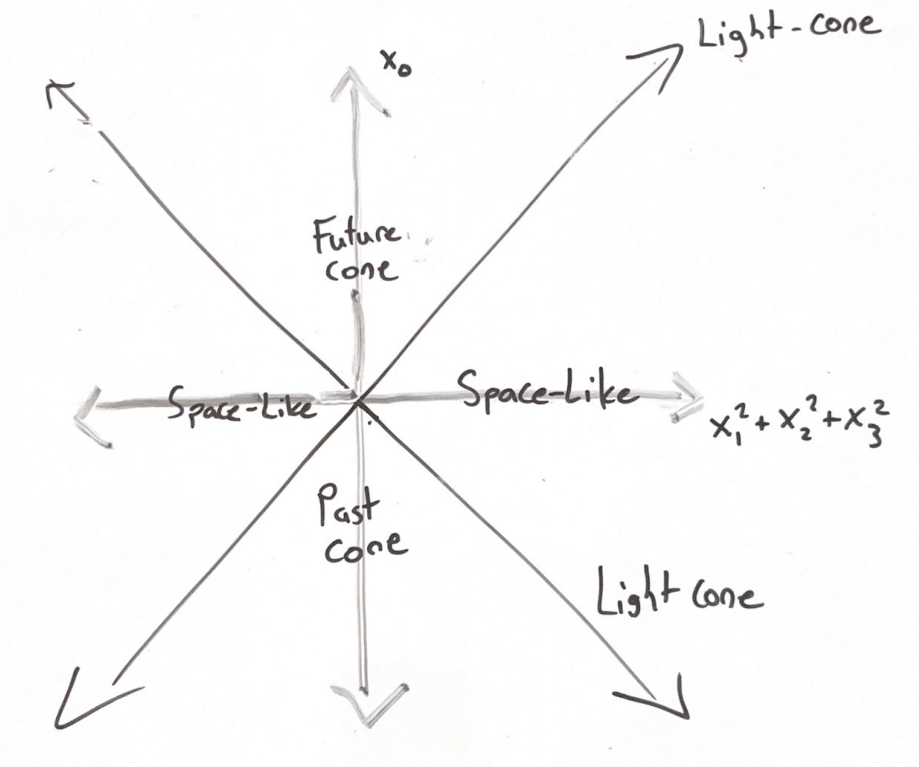
\includegraphics[width=0.7\textwidth]{Light cone-1}
	\caption{Decomposition of Minkowski Space based on length}
\end{figure}

In our study of many other groups in this thesis, group elements have been shown to have helpful decompositions that will make calculations more efficient. The proper Lorentz group is no exception to this.

\begin{theorem} \cite{Tung}
	Any $\Lambda \in \overset{\sim}{L}_+$ can be uniquely written in the following way:
$$\Lambda = R(\theta,\phi,0)L_z(\xi)R(\alpha,\beta,\gamma)^{-1}$$
where $L_z(\xi)$ is a Lorentz boost along the $z$-axis by angle $\xi$ and the parameters for the Euler angles of the rotations from $SO(3)$ are defined as expected.
\end{theorem}

For the sake of clarity, the proof is omitted, as it does not give insight into why this decomposition is possible. One can find more details here.\cite{Tung}

While we have covered what could be crudely considered rotations on Minkowski space, it is relatively straightforward to switch gears and now consider the translations on Minkowski space. Fortunately for us, the construction of these types of operations is very straightforward and is mostly omitted for simplicity. We define the translation group $T_4 = \{T_b \mid b\in\R^4\}$ in the most natural way. It is inherently abelian and will be used to aid us in defining a new group.

\begin{definition}
	The set of all compositions of translations proper Lorentz transformations is called the \textbf{Poincar\'e Group}, denoted $\overset{\sim}{P}$
\end{definition}

Generically speaking, for any transformation in $\overset{\sim}{P}$, any $x\in M$ is mapped into $x'$ in the following way:

\begin{equation}
\begin{aligned}
	x' = \Lambda x + b \text{ for some }\Lambda\in\overset{\sim}{L}_+ \text{ and } b\in\R^4
\end{aligned}
\end{equation}

Much like the Euclidean Group, the composition of any two $g(\Lambda,b),g(\Lambda',b')\in\overset{\sim}{P} $  can be seen to follow the equation below:

\begin{equation}
\begin{aligned}
g(\Lambda,b)g(\Lambda',b') = g(\Lambda\Lambda', \Lambda b' + b)
\end{aligned}
\end{equation}

It is easy to verify that we can embed any $g(\Lambda,b)$ into an invertible $5\times 5$ matrix that acts as the transformation defined by it (embedding four-vectors into a five dimensions space with a trivial component).

$$\begin{bmatrix}
	\underset{4\times 4}{\Lambda} & \underset{4\times 1}{b}\\
	\underset{1\times 4}{0} & \underset{1\times 1}{1}
\end{bmatrix}$$

It can also be easily verified that for any $g(\Lambda,b)\in\overset{\sim}{P}$, there is a natural decomposition of the transformation into:

\begin{equation}
\begin{aligned}
g(\Lambda,b)=T_b\Lambda
 \end{aligned}
\end{equation}


\noindent taking $T_b \sim g(I_4,b)$ and $\Lambda \sim g(\Lambda,0)$.

We can use this identity in a similar manner we did in the Euclidean Group to show that for any $T_b,\Lambda\in\overset{\sim}{P}$, we have

\begin{equation}
\begin{aligned}
	\Lambda T_b \Lambda^{-1} = T_{\Lambda b}
\end{aligned}
\end{equation}

\section{Irreducible Representations of The Poincar\'e Group}

Let us now establish our generators and the Lie Algebra associated with them.

We denote our translational generators $P_\mu$ where $\mu\in\{t,x,y,z\}$. These are defined using identical methodology to the construction of translational generators in $E_2$ and $E_3$. Explicitly, we can write 

\begin{center}
\begin{tabular}{cc}
	$P_t = \begin{bmatrix}
				0 & 0 & 0 & 0 & i \\
				0 & 0 & 0 & 0 & 0\\
				0 & 0 & 0 & 0 & 0\\
				0 & 0 & 0 & 0 & 0\\
				0 & 0 & 0 & 0 & 0\\
			\end{bmatrix}$ &
	$P_x = \begin{bmatrix}
				0 & 0 & 0 & 0 & 0 \\
				0 & 0 & 0 & 0 & i\\
				0 & 0 & 0 & 0 & 0\\
				0 & 0 & 0 & 0 & 0\\
				0 & 0 & 0 & 0 & 0\\
			\end{bmatrix}$ \\
	$P_y = \begin{bmatrix}
				0 & 0 & 0 & 0 & 0 \\
				0 & 0 & 0 & 0 & 0\\
				0 & 0 & 0 & 0 & i\\
				0 & 0 & 0 & 0 & 0\\
				0 & 0 & 0 & 0 & 0\\
			\end{bmatrix}$ &
	$P_z = \begin{bmatrix}
				0 & 0 & 0 & 0 & 0 \\
				0 & 0 & 0 & 0 & 0\\
				0 & 0 & 0 & 0 & 0\\
				0 & 0 & 0 & 0 & i\\
				0 & 0 & 0 & 0 & 0\\
			\end{bmatrix}$
\end{tabular}
\end{center}

and given this, we write any pure translation in $\overset{\sim}{P}$ as 

\begin{equation}
\begin{aligned}
	T_b = e^{-ib_1P_t}e^{-ib_2P_x}e^{-ib_3P_y}e^{-ib_4P_z}
\end{aligned}
\end{equation}

It can then be easily verified with matrix algebra that for any Lorentz transformation (embedded in $M_5(\R)$) the translational generators exhibit the following behavior:

\begin{equation}
\begin{aligned}
	\Lambda P_t \Lambda^{-1} = [\Lambda]_{00}P_t + [\Lambda]_{10}P_x + [\Lambda]_{20}P_y + [\Lambda]_{30}P_z
\end{aligned}
\end{equation}
\begin{equation}
\begin{aligned}
	\Lambda P_x \Lambda^{-1} = [\Lambda]_{01}P_t + [\Lambda]_{11}P_x + [\Lambda]_{21}P_y + [\Lambda]_{31}P_z
\end{aligned}
\end{equation}
\begin{equation}
\begin{aligned}
	\Lambda P_y \Lambda^{-1} = [\Lambda]_{02}P_t + [\Lambda]_{12}P_x + [\Lambda]_{22}P_y + [\Lambda]_{32}P_z
\end{aligned}
\end{equation}
\begin{equation}
\begin{aligned}
	\Lambda P_z \Lambda^{-1} = [\Lambda]_{03}P_t + [\Lambda]_{13}P_x + [\Lambda]_{23}P_y + [\Lambda]_{33}P_z
\end{aligned}
\end{equation}

This should feel like a familiar relationship as we derived in the Euclidean Group (and would likely be the case if we had discussed $E_4$). However, this should allude to the fact that the translational subgroup is intuitively invariant under rotations, and will later be used to search for our invariant subspace. 

We now shift our focus to our generators for rotations. For now, we will consider pure spatial rotations separately from rotations involving a time component. In this sense, we can keep our naming convention by denoting the rotational generator $J_\mu$ where $\mu\in\{x,y,z\}$ to be the rotation about the $\mu$ axis in $\R^3$. Through our similar derivation in $SO(3)$, we recover the following matrices for our generators:


\begin{center}
\begin{tabular}{ccc}
	$J_x = \begin{bmatrix}
				0 & 0 & 0 & 0 & 0 \\
				0 & 0 & 0 & 0 & 0\\
				0 & 0 & 0 & -i & 0\\
				0 & 0 & i & 0 & 0\\
				0 & 0 & 0 & 0 & 0\\
			\end{bmatrix}$ &
	$J_y = \begin{bmatrix}
				0 & 0 & 0 & 0 & 0 \\
				0 & 0 & 0 & i & 0\\
				0 & 0 & 0 & 0 & 0\\
				0 & -i & 0 & 0 & 0\\
				0 & 0 & 0 & 0 & 0\\
			\end{bmatrix}$ &
	$J_z = \begin{bmatrix}
				0 & 0 & 0 & 0 & 0 \\
				0 & 0 & -i & 0 & 0\\
				0 & i & 0 & 0 & 0\\
				0 & 0 & 0 & 0 & 0\\
				0 & 0 & 0 & 0 & 0\\
			\end{bmatrix}$ 
\end{tabular}
\end{center}

Handling the generators of the Lorentz boosts ultimately takes the same form as we have already established. Using the arbitrarily small angle of rotation to create two different ways of computing a generic element, we uncover the following form for our generators of Lorentz boosts: Let $K_m$ where $m\in\{x,y,z\}$ denote the generator of the Lorentz boost along the $m$ axis. Then,

\begin{center}
\begin{tabular}{ccc}
	$K_x = \begin{bmatrix}
				0 & i & 0 & 0 & 0 \\
				i & 0 & 0 & 0 & 0\\
				0 & 0 & 0 & 0 & 0\\
				0 & 0 & 0 & 0 & 0\\
				0 & 0 & 0 & 0 & 0\\
			\end{bmatrix}$ &
	$K_y = \begin{bmatrix}
				0 & 0 & i & 0 & 0 \\
				0 & 0 & 0 & 0 & 0\\
				i & 0 & 0 & 0 & 0\\
				0 & 0 & 0 & 0 & 0\\
				0 & 0 & 0 & 0 & 0\\
			\end{bmatrix}$ &
	$K_z = \begin{bmatrix}
				0 & 0 & 0 & i & 0 \\
				0 & 0 & 0 & 0 & 0\\
				0 & 0 & 0 & 0 & 0\\
				i & 0 & 0 & 0 & 0\\
				0 & 0 & 0 & 0 & 0\\
			\end{bmatrix}$ 
\end{tabular}
\end{center}

As would be expected, any Lorentz transformation can be written in terms of the generators in the following way:

\begin{equation}
\begin{aligned}
	\Lambda (\omega) = e^{-i\omega_1J_x}e^{-i\omega_2J_y}e^{-i\omega_3J_x}e^{-i\omega_4K_x}e^{-i\omega_5K_y}e^{-i\omega_6K_z}
\end{aligned}
\end{equation}

\noindent where $\omega$ is a six-component vector containing values appropriately assigned that decompose $\Lambda$ into rotations in the specified planes. This decomposition can be arrived at with more work using Theorem (5.7). 

At this stage, we can construct a generic element of our Lie algebra, $\mathfrak{\overset{\sim}{p}}$ in the following way. If $A\in\mathfrak{\overset{\sim}{p}}$, 

\begin{equation}
\begin{aligned}A=i
	\begin{bmatrix}
		0 & a & b & c & d\\
		a & 0 & -h & j & e\\
		b & h & 0 & -k & f\\
		c & -j & k & 0 & g\\
		0 & 0 & 0 & 0 & 0\\
	\end{bmatrix}
\end{aligned}
\end{equation}

We can now establish the following commutator relationships through matrix algebra

\begin{equation}
\begin{aligned}
	[P_\mu,P_\nu] = 0 \hspace{3mm} \forall \mu,\nu\in\{t,x,y,z\}
\end{aligned}
\end{equation}
\begin{equation}
\begin{aligned}
	[P_t,P_\mu] = 0 \hspace{3mm} \forall \mu\in\{x,y,z\}
\end{aligned}
\end{equation}
\begin{equation}
\begin{aligned}
	[P_\mu,J_\nu] = \begin{cases}
							0 &\text{if } \mu=\nu \\
							isign(\mu,\nu,\tau)P_\tau & \text{else}
						\end{cases} \hspace{3mm} \forall \mu,\nu,\tau\in\{x,y,z\}\text{ where }\tau \neq\mu,\nu
\end{aligned}
\end{equation}
\begin{equation}
\begin{aligned}
	[P_\mu,K_\nu] = \begin{cases}
							0 &\text{if } \mu=\nu \\
							iP_t & \text{else}
						\end{cases} \hspace{3mm} \forall \mu,\nu\in\{x,y,z\}
\end{aligned}
\end{equation}
\begin{equation}
\begin{aligned}
	[P_t,K_\nu] = iP_\nu \hspace{3mm} \forall\nu\in\{x,y,z\}
\end{aligned}
\end{equation}
\begin{equation}
\begin{aligned}
	[J_\mu,J_\nu] = \begin{cases}
							0 &\text{if } \mu=\nu \\
							isign(\mu,\nu,\tau)J_\tau & \text{else}
						\end{cases} \hspace{3mm} \forall \mu,\nu,\tau\in\{x,y,z\}\text{ where }\tau \neq\mu,\nu
\end{aligned}
\end{equation}
\begin{equation}
\begin{aligned}
	[K_\mu,J_\nu] = \begin{cases}
							0 &\text{if } \mu=\nu \\
							isign(\mu,\nu,\tau)K_\tau & \text{else}
						\end{cases} \hspace{3mm} \forall \mu,\nu,\tau\in\{x,y,z\}\text{ where }\tau \neq\mu,\nu
\end{aligned}
\end{equation}
\begin{equation}
\begin{aligned}
	[K_\mu,K_\nu] = \begin{cases}
							0 &\text{if } \mu=\nu \\
							-isign(\mu,\nu,\tau)J_\tau & \text{else}
						\end{cases} \hspace{3mm} \forall \mu,\nu,\tau\in\{x,y,z\}\text{ where }\tau \neq\mu,\nu
\end{aligned}
\end{equation}

In order to calculate the unitary, irreducible representations of the Poinecar\'e group, we must utilize the same method we used for calculating such representations of $E_3$. To begin, we identify a natural choice for a normal subgroup to quotient out. The easy choice would be $T_4$. Since all the generators of $T_4$ commute, we can conclude that their eigenvectors through the image of any irreducible representation coincide. We sojourn into the universal enveloping algebra to acquire our Casimir elements. In this case, we start by defining a new yet familiar element:

 
\begin{equation}
\begin{aligned}
	\mathfrak{C}_1 \coloneq \mathfrak{P}_t^2 -  \mathfrak{P}_x^2 -\mathfrak{P}_y^2- \mathfrak{P}_z^2
\end{aligned}
\end{equation}

If we assert that $\psi$ is an irreducible representation of $\overset{\sim}{P}$, then we see we see that any eigenvalue of $\psi_{\mathfrak{C}_1}$ need not be strictly positive. Let us denote this eigenvalue as $\lambda_1$. We make note of the ranges for the $\lambda_1$ and separate our tabulation into three cases. For the sake of this thesis, we will only compute the irreducible unitary representations for one of these cases. The rest require work with a more complicated Casimir element than we are used to.

Our case of focus will be when $\lambda_1 > 0$. This means that the time component must be larger in magnitude than all of the spatial components combined. This corresponds to vectors that are time-like. To this end, we pick our starting vector to be $v_0 \coloneq (\sqrt{\lambda_1},0,0,0)$. Taking our anticipated quotient, we can intuitively see that $\overset{\sim}{P}/T_4 \cong \overset{\sim}{L}_+$. We can also see that the largest possible subgroup of this quotient group that leaves time-like vectors invariant would need to be the subgroup isomorphic to $SO(3)$. Therefore, since our little group is isomorphic to $SO(3)$ we will see that every irreducible, unitary representation of $SO(3)$ gives rise to one in $\overset{\sim}{P}$. We recall that for any half or whole positive integer choice of $s$, then we can construct a basis of the subspace corresponding to the image of the little group under $\psi$ in the following way:

\begin{equation}
\begin{aligned}
	\psi_{\mathfrak{J}^2} (v_0)_m = s(s+1)(v_0)_m
\end{aligned}
\end{equation}
\begin{equation}
\begin{aligned}
	\psi_{\mathfrak{J}_z} (v_0)_m = m(v_0)_m
\end{aligned}
\end{equation}
\begin{equation}
\begin{aligned}
	\psi_{\mathfrak{P}_\mu} (v_0)_m = \begin{cases}
										\sqrt{\lambda_1} & \text{if } \mu=t\\
										0 & \text{else}
										\end{cases}
\end{aligned}
\end{equation}

In order to collect a bigger subspace invariant under $\psi$, we deform our initial vector through a general Lorentz transformation. This is straightforward to compute since we have a nice general decomposition of such transformation as seen in (5.7). However, the right-most component of the decomposition of this transformation leaves our vectors invariant (since it is part of $SO(3)$). For clarity, we define a transformation of the following form:

\begin{equation}
\begin{aligned}
	v_p\coloneq H_p((v_0)_m)= R(\alpha,\beta,0)L_z(\xi)(v_0)_m
\end{aligned}
\end{equation}

where ($\alpha$,$\beta$) are the cylindrical coordinates identifying the three-dimensional components of the four-vector $v_p$. This transformation can be applied to change our reference vector to any other vector in $M$. We can generalize the above analysis on each subspace that arises from the little group corresponding to $p$. We recover the entire space by letting $p$ be arbitrary.

\begin{theorem} Time-like Unitary Irreducible Representations of $\overset{\sim}{P}$
	The subspace generated by the vectors $\{(v_p)_m\}_{p,m}$ is invariant under $\overset{\sim}{P}$. The irreducible, unitary representations of elements of this group are characterized in the following way:
$$\psi_{T_b} (v_p)_m = e^{-ib_0p_0}e^{-ib_1p_1}e^{-ib_2p_2}e^{-ib_3p_3}(v_p)_m$$
$$\psi_\Lambda (v_p)_m = [\phi_s(H(p')\Lambda H(p))]_{m'm} (v_{p'})_{m'}$$
where $p' = \Lambda p$ and $\phi_s$ is the irreducible representation of $SO(3)$ defined by $s$.
\end{theorem}

This can be shown in a very similar manner to the methods used in the Euclidean Groups' calculations. 




\chapter{The Braid Group and Anyons}\label{braids}

For our last group of study, we will focus our attention to a group of quite unique construction. We seek to make the idea of a braiding mathematically rigorous. We will be taking $n$ strands and tying them around each other to form new objects within our group. While this inherently concrete idea is our main goal to study, we require lots of rigorous mathematics to develop this concept sufficiently. Our ultimate goal is to begin characterization of a special kind of quasiparticle known as anyons. It turns out that when systems of anyons go through a processes that exchange their position, they exhibit behavior that resembles the structure of braids. We will utilize our study of representation theory to both study anyons through the perspective of braids and then study braids from the perspective of anyons. This chapter follows the structure of multiple sources, including Christian Kassel's \textit{Braid Groups}, Avinash Deshmukh's \textit{An Introduction to Anyons}, and Simon Trebst's \textit{A Short Introduction to Fibonacci Anyon Models}. \cite{Kassel,Deshmukh,Trebst}

\section{Construction of the Braid Group}

There are multiple ways to construct the braid group. While our instincts are to do so with the image of intertwined strings, we have to first a more algebraic definition to begin with.

\begin{definition}
	The braid group, $B_n$, is generated by $n-1$ generators (denoted $\sigma_1,\hdots,\sigma_{n-1}$) that have the following "braid relations":
$$\sigma_i\sigma_j = \sigma_j\sigma_i \hspace{3mm} \forall i,j \in \{1,\hdots,n-1\} \text{ where } |i-j|>1$$
$$\sigma_i\sigma_{i+1}\sigma_i=\sigma_{i+1}\sigma_i\sigma_{i+1} \hspace{3mm} \forall i \in \{1,\hdots,n-2\}$$
\end{definition}

These relations are somewhat daunting at first glance, but we can identify the braid group with a familiar group through the lens of a homomorphism to give us an easier interpretation for now. Consider the following map:

$$\phi:B_n\rightarrow S_n$$
$$\sigma_k \mapsto (k \hspace{2mm} k+1)$$

\noindent where $(k \hspace{2mm}k+1)$ is cycle notation for the transposition that swaps $k$ and $k+1$. This map can be shown to be a homomorphism, but most importantly, this map perserves the braid relations. That is to say, the transpositions of $S_n$ adhere to the braid relations. However we must be wary; these two groups are not the same. Namely, this is a result of the fact that every transposition is its own inverse in $S_n$ and none of the generators of $B_n$ are their own inverses. 

While this is a good way to get our bearings in the algebraic richness of the braid group, we can also construct this group in a more topological sense.

\begin{definition}
	A \textbf{geometric braid} on $n\in \N$ strands is a set $b\subset\R^2\times [0,1]$ formed by $n$ disjoint, intervals topologically equivalent to $[0,1]$ such that we can define a projection mapping from $\R^2\times [0,1]$ to $[0,1]$ that maps each strand homeomorphically to $[0,1]$ and the following conditions hold:
$$b\cap(\R^2\times\{0\}) = \{(1,0,0),(2,0,0),\hdots,(n,0,0)\}$$
$$b\cap(\R^2\times\{1\}) = \{(1,0,1),(2,0,1),\hdots,(n,0,1)\}$$
\end{definition}

\begin{figure}[H]
	\centering
	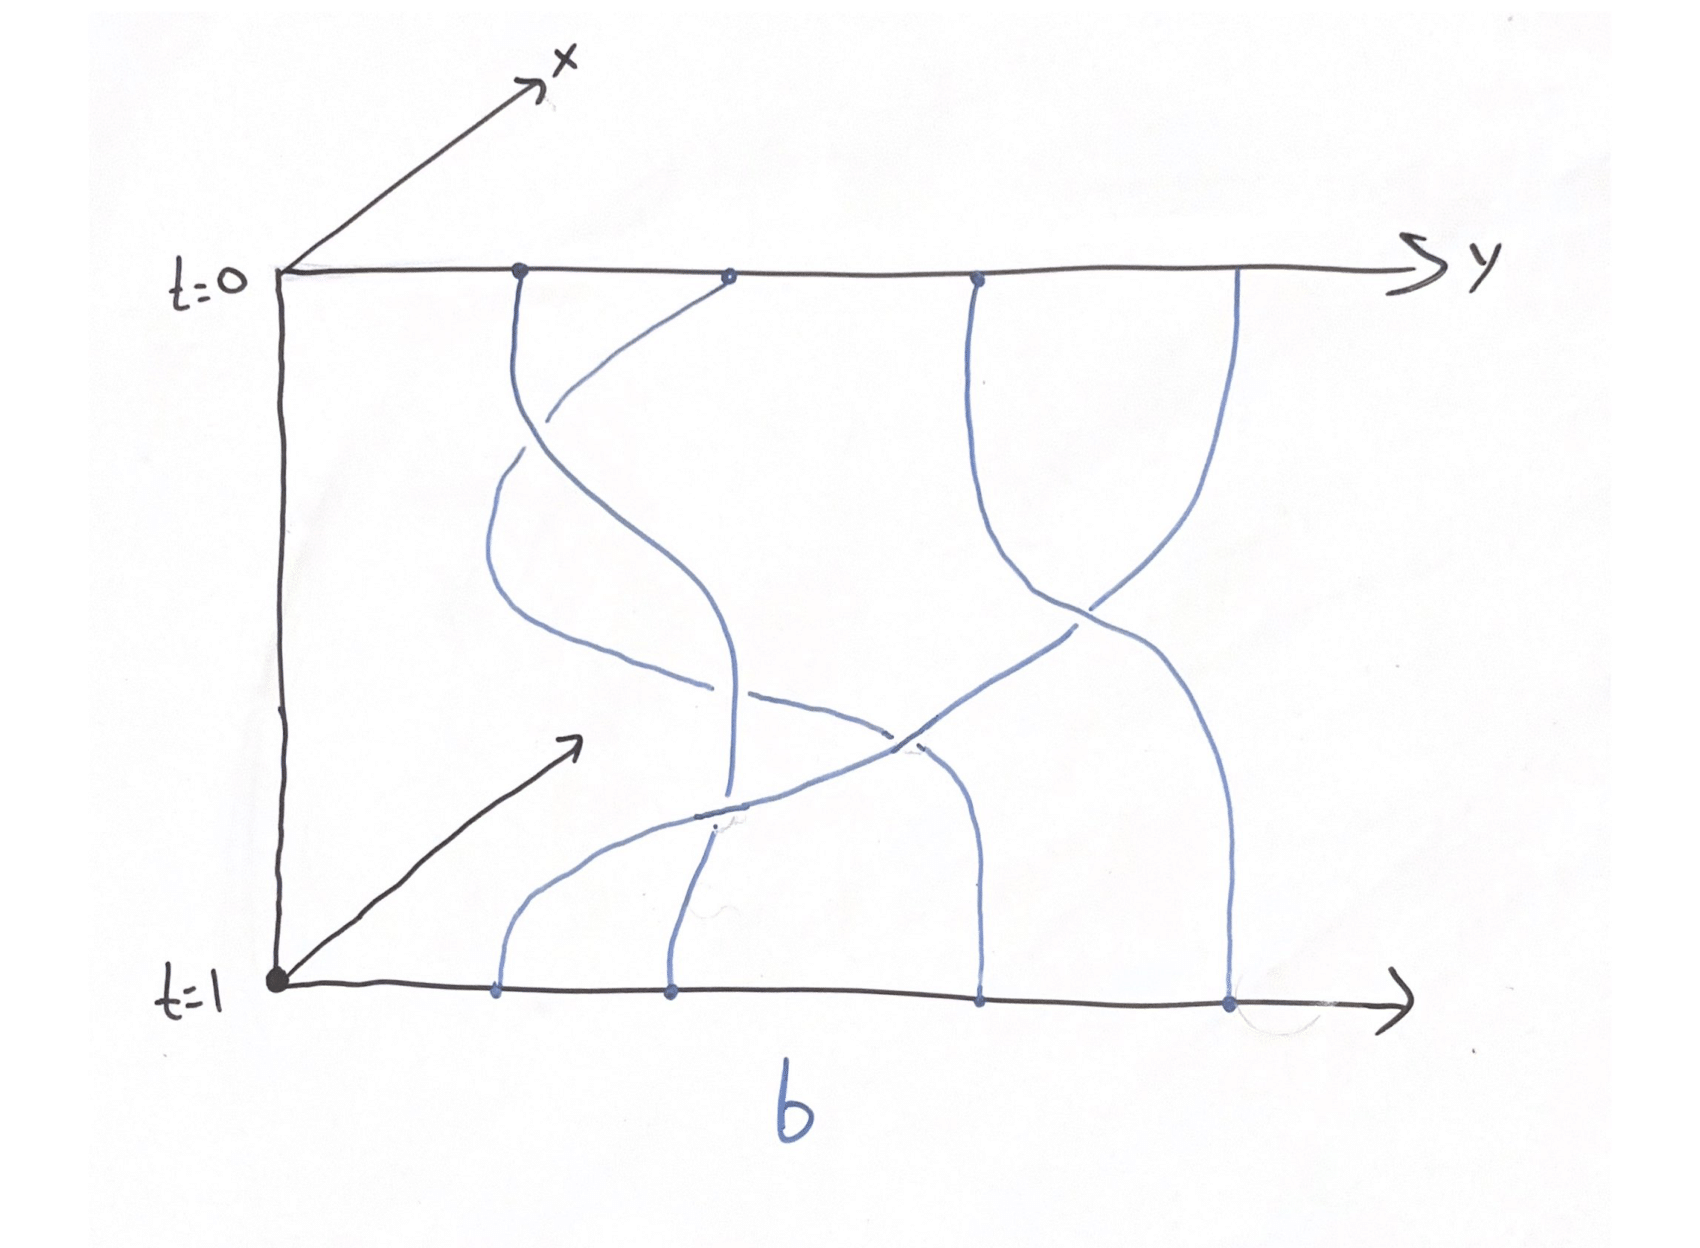
\includegraphics[width=0.7\textwidth]{geobraid.png}
	\caption{Generic geometric braid}
\end{figure}

Based on this construction of a braid, we can immediately notice a few properties. First, every stand will intersect a level curve of this set at exactly one point (otherwise the stands are not homeomorphic to $[0,1]$). Further, every strand can be traveled as a path, having a unique start and end point. If each strand begins at the point $(n,0,0)$ and ends at $(n',0,1)$, then we can construct a permutation in $S_n$ that captures the behavior of this transition (from $n$ to $n'$). We call such a permutation the underlying permutation of $b$.

\begin{definition}
	Two braids, $b_1$ and $b_2$, are said to be \textbf{isotopic} to each other if one can be continuously deformed into the other. This is an equivalence relation.
\end{definition}

We can define the product between two braids heuristically and formally. Crudely, the product of two braids is defined to be the stacking of one braid on top of the other, lining up the start and end points. More formally, if $b_1$ and $b_2$ are two geometric braids, we define 

\begin{equation}
\begin{aligned}
	b_1b_2 \coloneq \{(x,y,t)\mid (x,y,2t)\in b_1 \text{ when }0\leq t\leq \frac{1}{2} \text{ and }   (x,y,2t - 1)\in b_2 \text{ when }\frac{1}{2}\leq t\leq 1\}
\end{aligned}
\end{equation}

\begin{figure}[H]
	\centering
	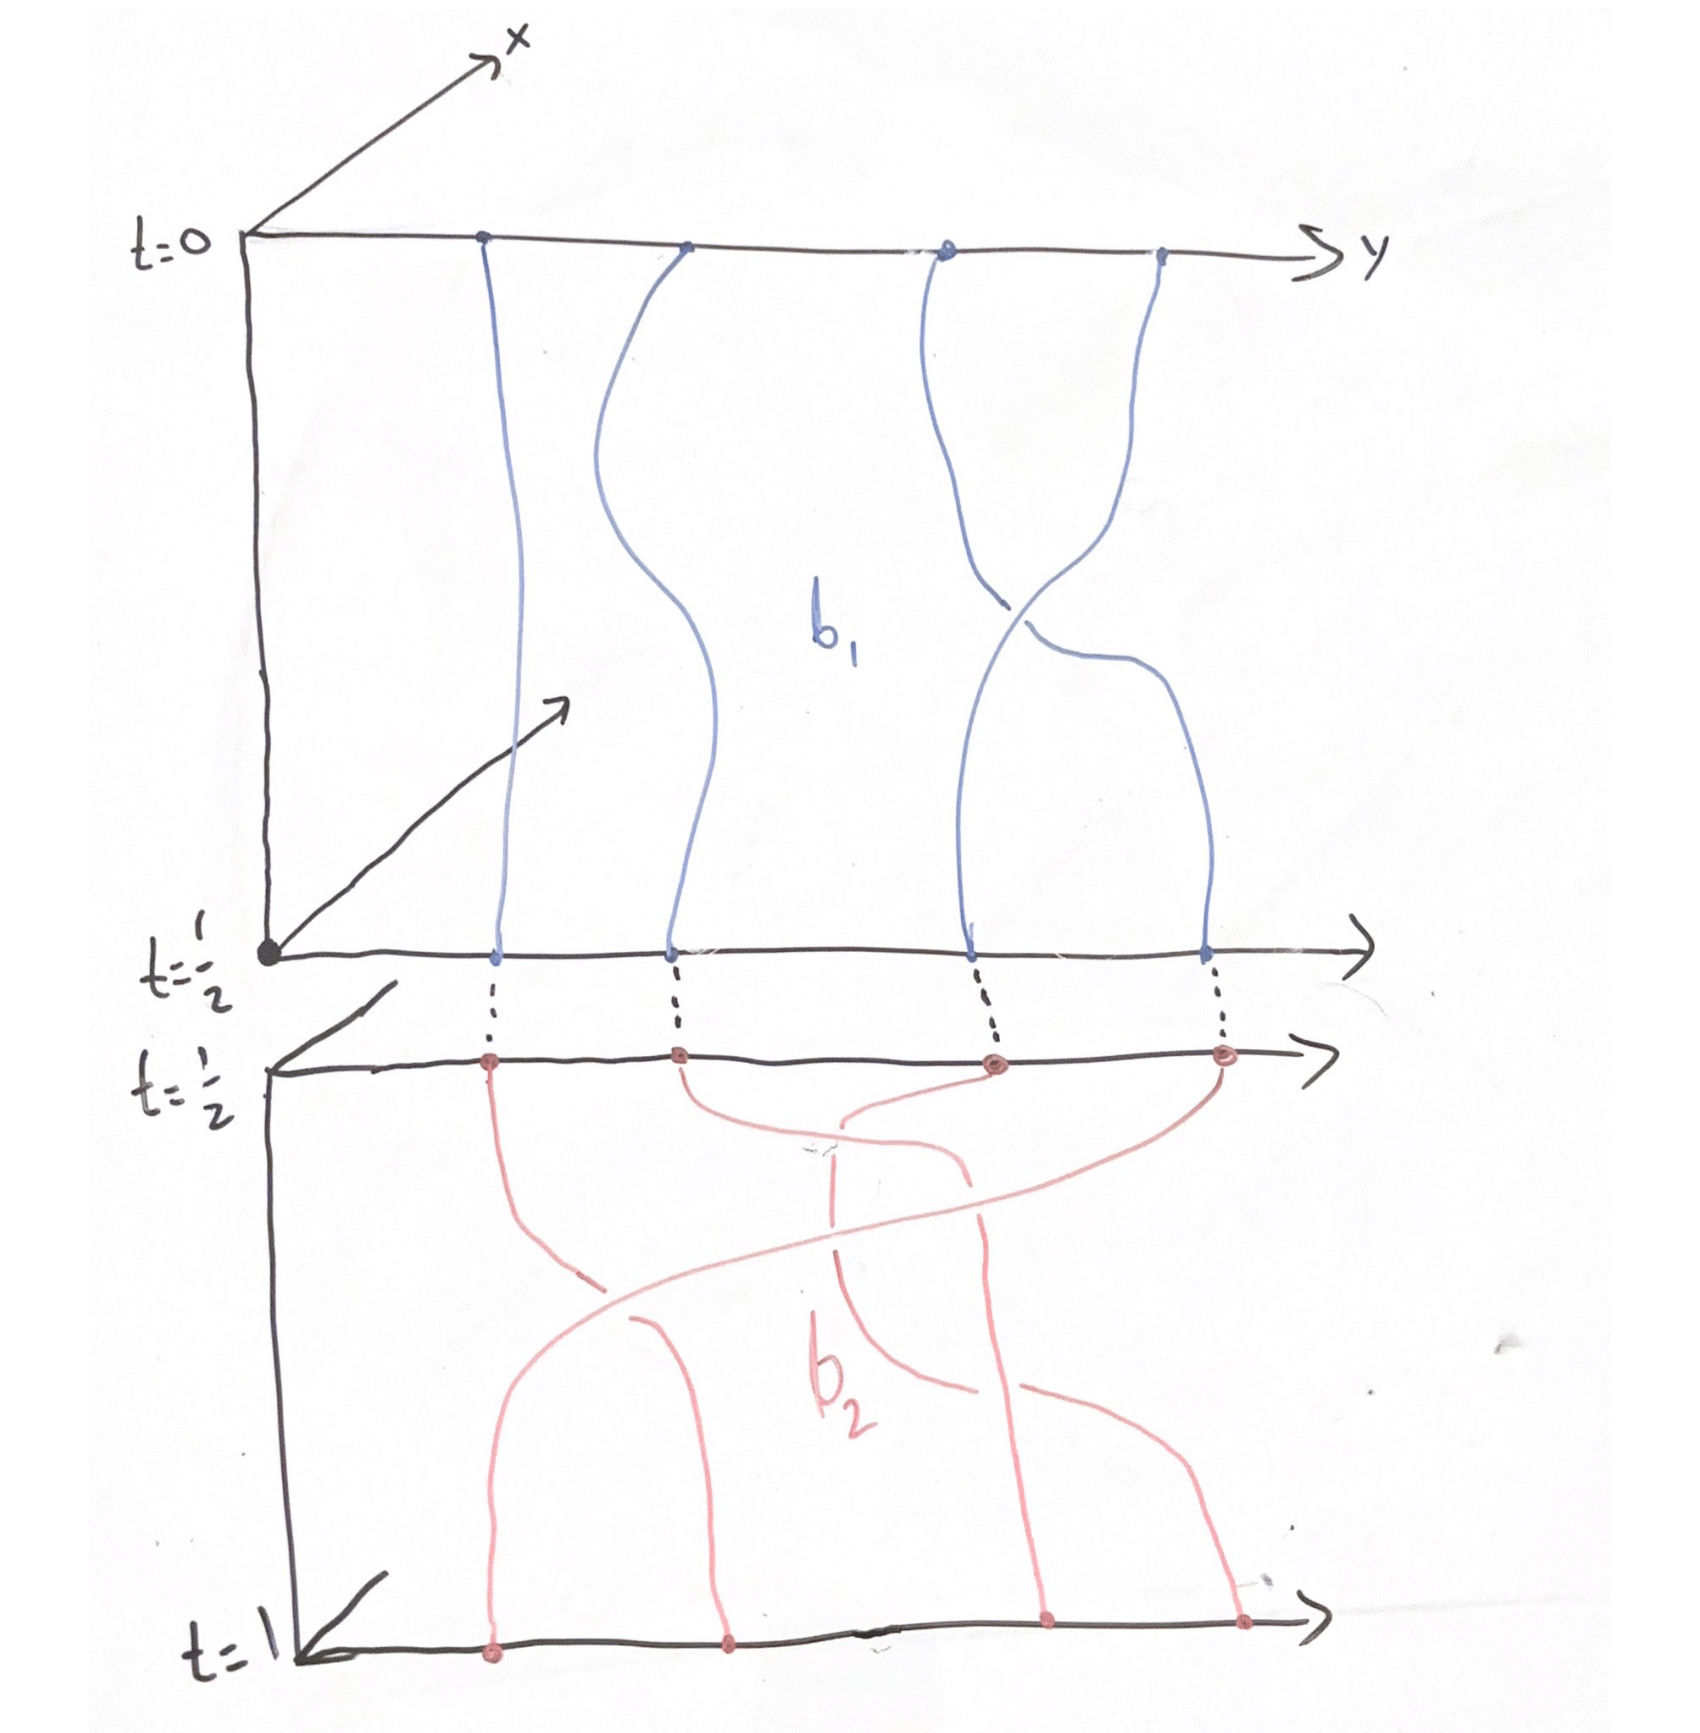
\includegraphics[width=0.7\textwidth]{geobraidprod.png}
	\caption{The product of two geometric braids.}
\end{figure}

This operation is clearly associative, and there is an identity element corresponding to the geometric braid that does not wrap any strands around one another. Hence, the collection of all geometric braids forms a group. To avoid any unecessary craziness, we will work on the group of equivalence classes of geometric braids. We will work towards establishing the connection the canonical braid group $B_n$ and the group of geometric braids.

In order to visualize more easily, we will formally introduce the concept of a braid diagram.

\begin{definition}
	A \textbf{braid diagram} on $n$ strands is set, $\mathcal{D}\subset \R\times [0,1]$ made up as a union of $n$ intervals topologically equivalent to $[0,1]$ (called strands) such that the following conditions are met:
\begin{itemize}
	\item There exists a projection map from $\R\times [0,1]$ to $[0,1]$ that maps each strand homeomorphically to $[0,1]$.
	\item Every element of $\{1,2,\hdots,n\}\times\{0,1\}$ is a starting or endpoint of a unique strand.
	\item Every element in $\mathcal{D}$ belongs to either one or two strands. When an elment belongs to two, one strand must be designated as overgoing and the other undergoing (referred to as a crossing of $\mathcal{D}$
\end{itemize}
\end{definition}

We can make an intuitive identification of geometric braids with braid diagrams by thinking of the latter as a projection of the former onto the $xt$-plane ($t$ representing the interval $[0,1]$). Identifying a geometric braid with a braid diagram takes the diagram and at every crossing, splits the strands in such a way that the undergoing strand gets placed ``behind" the overgoing strand, which there is plenty of room to do in $\R$.

Much like the braids the that braid diagrams represent, two braid diagrams are said to be isotopic if one can be continuously deformed into the other. Further, we can define a product on braid diagrams as well in an identical process that we did to define it on the braids. The product of two braid diagrams visually resembles stacking two diagrams on top of each other. In this way, we can  identify the group of geometric braids with a carefully group of braid diagrams (of course defined on equivalency classes in both settings). 

However, these groups are not necessarily isomorphic. When projecting down in onto a two-dimensional surface, we lose information about the geometric braid. There is potential to confuse two braid diagrams as representing different geometric braids when in reality they represent an isotopic geometric braid.

\begin{figure}[H]
	\centering
	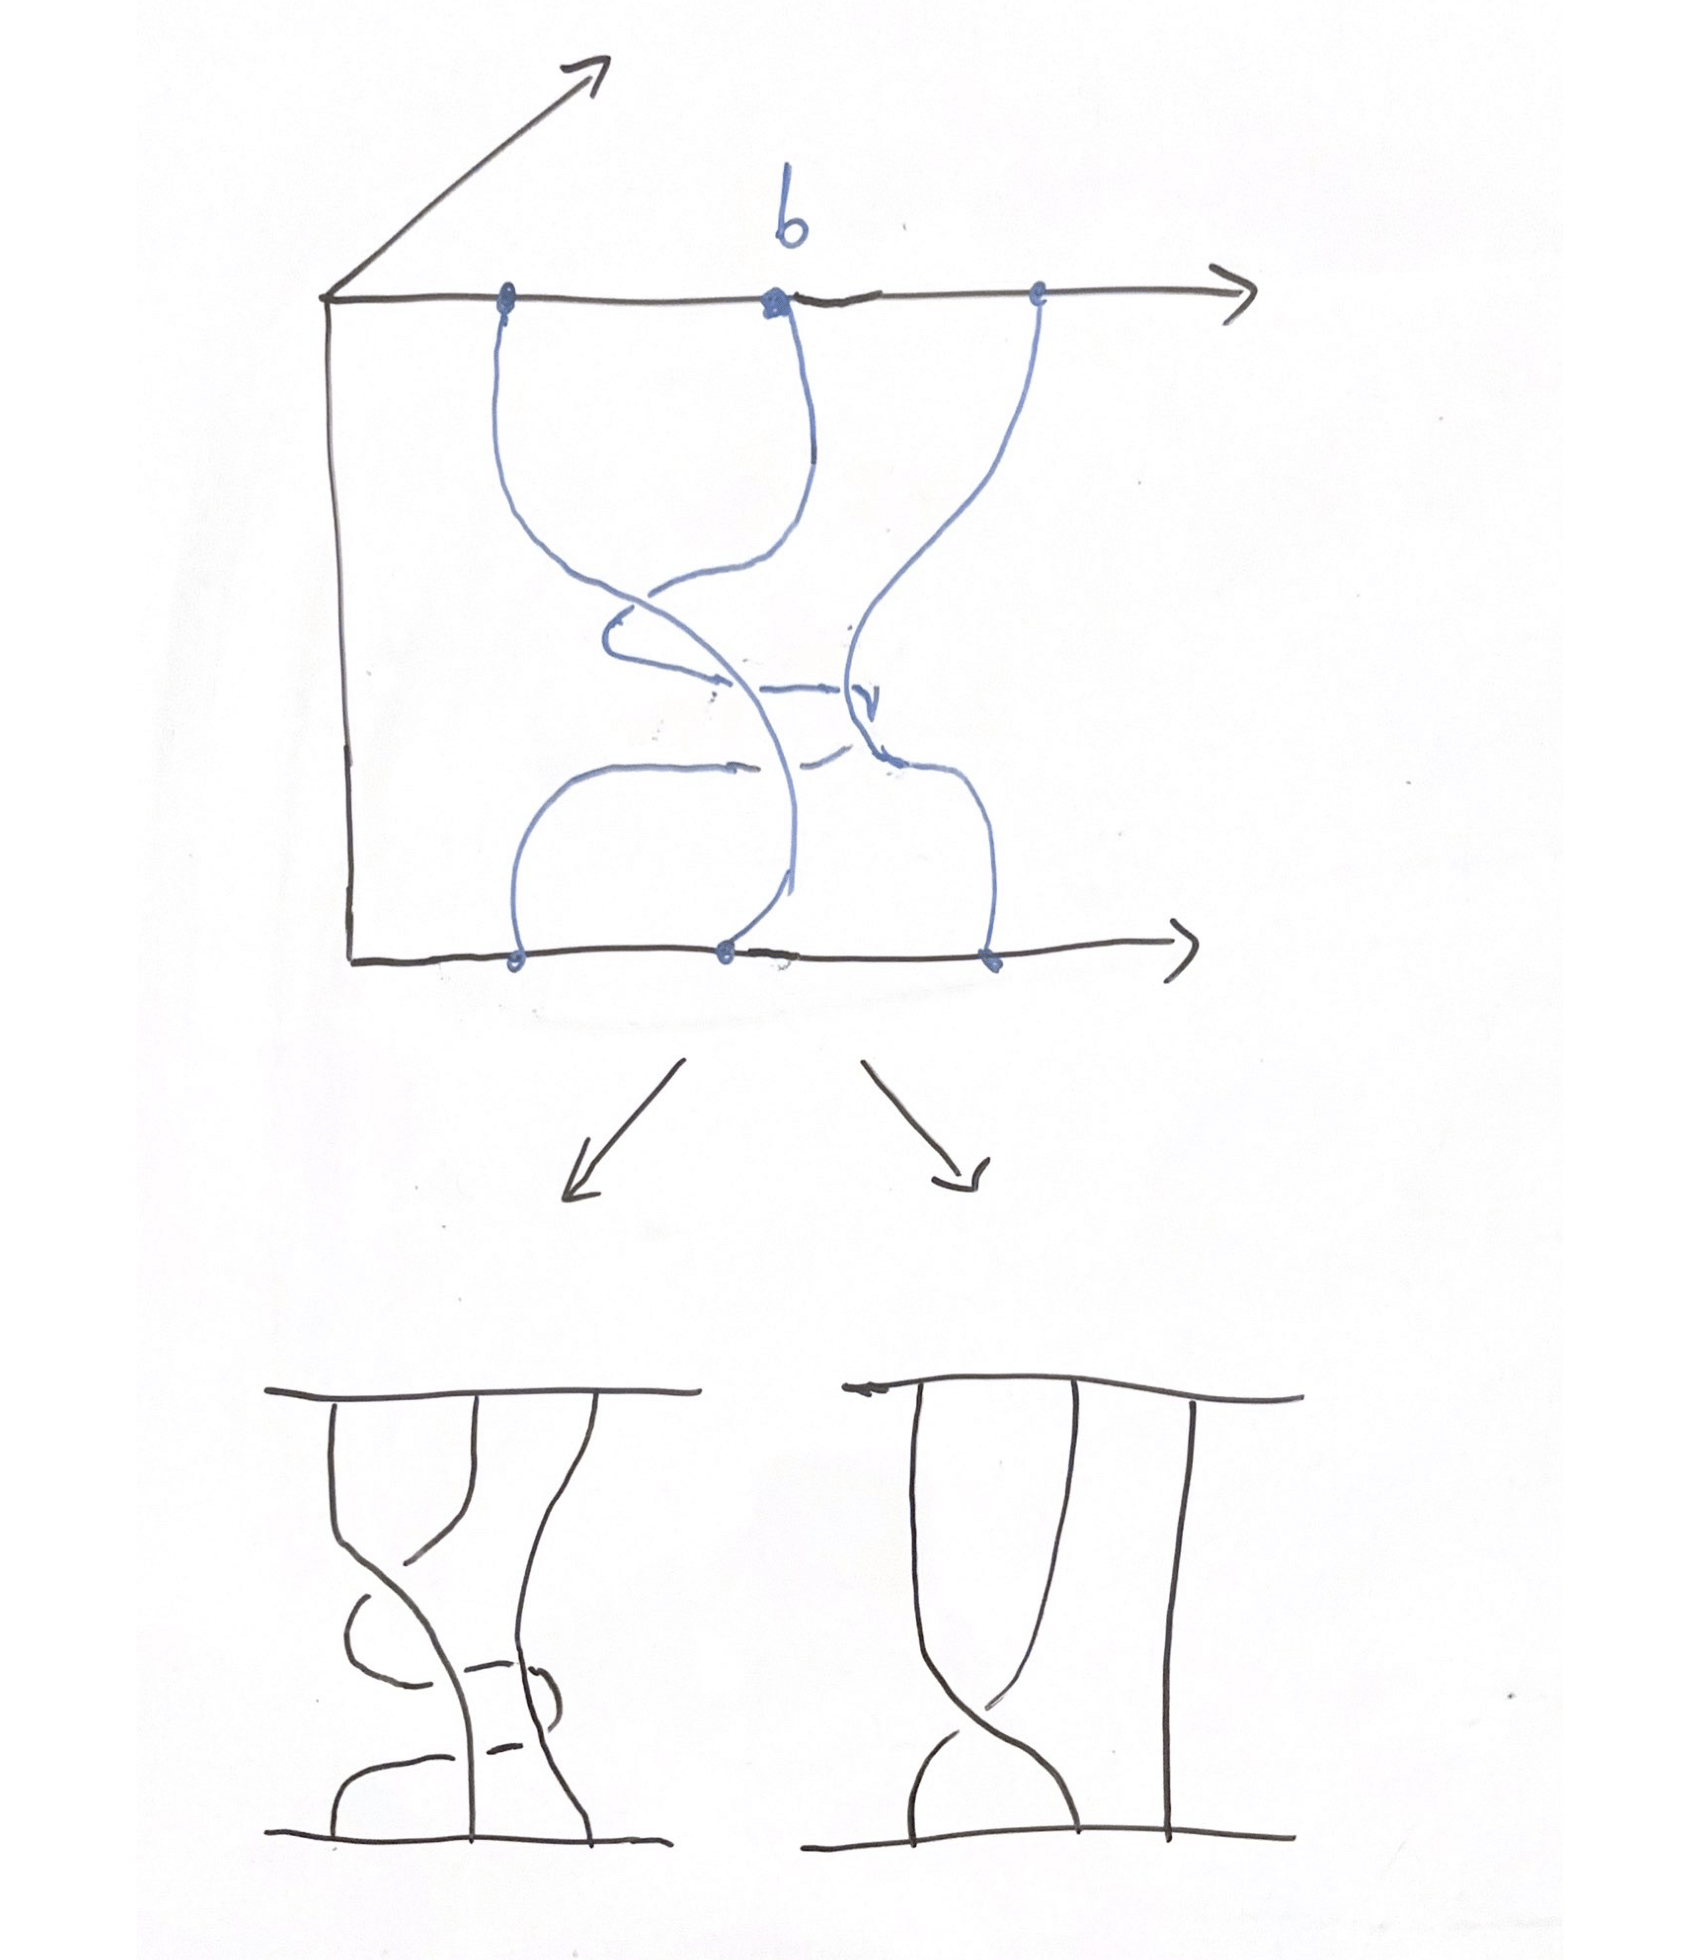
\includegraphics[width=0.7\textwidth]{requiv.png}
	\caption{Two braid diagrams that correspond to the same geometric braid.}
\end{figure}

We appeal to the Reidemeister moves developed in Knot Theory to aid us in our ability to detect when braid diagrams represent the same geometric braid. There are two specific types of moves we will reference.

Our first kind Reidemeister move to be consider will be given the label $\Omega$. Applying the move $\Omega$ to two adjacent strands of a braid does the following: First, it chooses one strand to be the overgoing strand and the other to be the undergoing strand. Then it takes the overgoing strand and creates two crossings by moving part of the strand over and across the other strand. There are two crossings because the strands are not switching positions, meaning the path the strand makes must return back the way it came. Note that we have to make a choice about which strand is under-versus-overgoing, and so we will take the convention that $\Omega_1$ is the move that favors the left strand as overgoing and $\Omega_2$ is the move that favors the right as overgoing. The inverses of both these moves are also Reidemeister moves.

\begin{figure}[H]
	\centering
	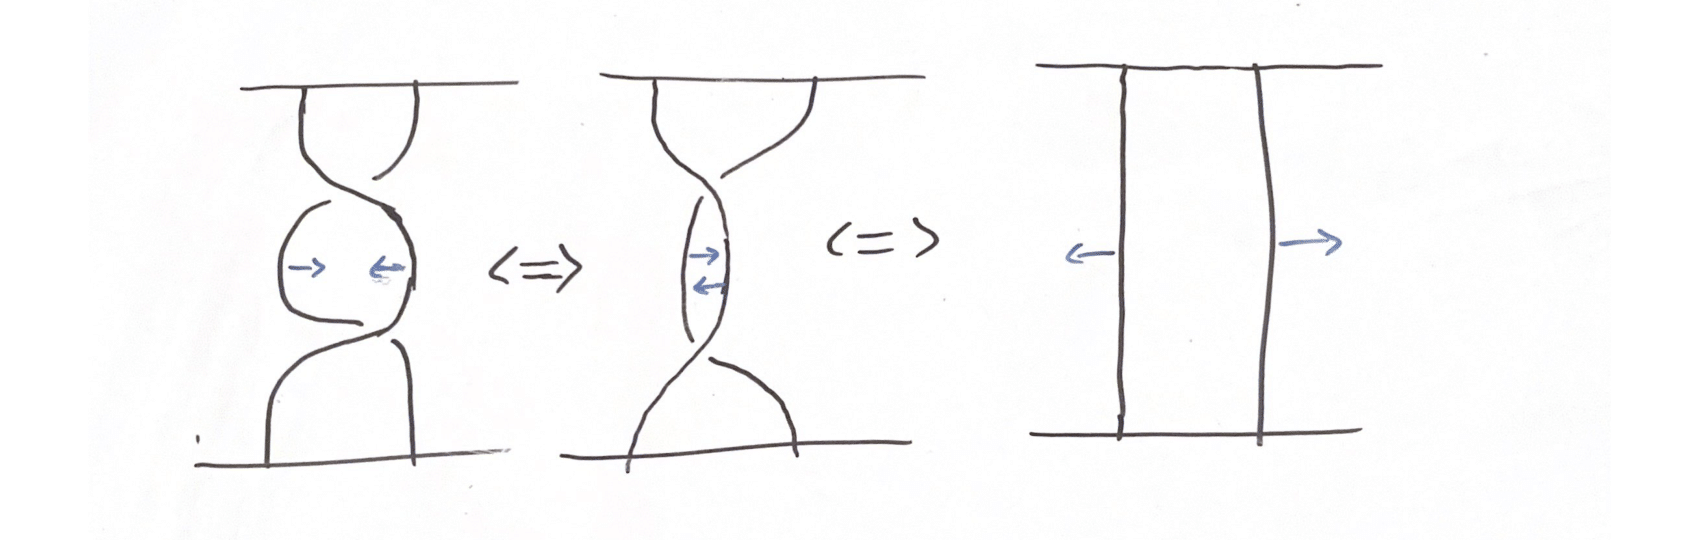
\includegraphics[width=0.7\textwidth]{reidmove2.png}
	\caption{$\Omega_1^{-1}$}
\end{figure}

Our second kind of Reidemeister move will be given the label of $\Theta$. In order to execute this move, we require there be three adjacent strands. Further we need one strand to cross both other strands in the same manner (simultaneously under-or-overgoing) and that the remaining two strands cross in an unspecified manner. The move $\Theta$ will take the one strand that under/overgoes both and moves it under/over the crossing of the other two strands to the other side. 

\begin{figure}[H]
	\centering
	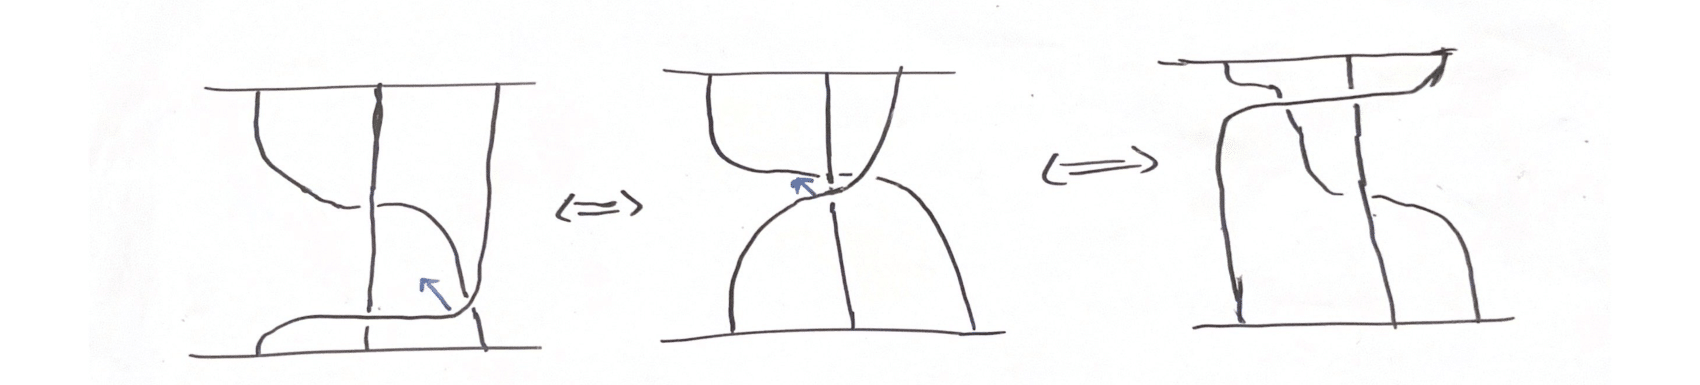
\includegraphics[width=0.7\textwidth]{reidmove3.png}
	\caption{$\Theta$}
\end{figure}

\begin{definition}
	Two braid diagrams are said to be \textbf{R-equivalent} if one can be transformed into the other by means of a finite sequence of isotopies and Reidemeister moves.
\end{definition}

R-equivalence is naturally an equivalence relation, and if we consider the quotient space of the group of braid diagrams, we get a group isomorphic to the group of geometric braids.

Now, all that is left to do is connect our geometric braids back to the algebraic definition. We can start by considering the braid diagrams of our geometric braids. If we are considering braids on $n$ strands, then we define $\sigma_i^+$ to be the braid diagram where the only crossing is the $i^{th}$ strand crossing under the $i+1^{th}$ strand and $\sigma_i^-$ to be the braid diagram where the only crossing is the $i^{th}$ strand crossing over the $i+1^{th}$ strand. We define this for ever $i\in\{1,2,\hdots,n-1\}$. Then the following holds:

\begin{theorem}
	Let $\mathcal{B}_n$ be the group of geometric braids on $n$ strands. Then for any $\beta\in\mathcal{B}_n$, $\beta$ has a natural decomposition:
$$\beta = \sigma^{\epsilon_1}_{i_1}\hdots\sigma^{\epsilon_k}_{i_k}$$ 
where $i_1,i_2,\hdots,i_k\in\{1,2,\hdots,n-1\}$ and $\epsilon_i = \pm$
\end{theorem}

\noindent \begin{proof}[\cite{Kassel}] Let $D(\beta)$ be the braid diagram of $\beta$. Then, we can create a partition of the interval $[0,1]$ in such a way that for every subinterval indicated by the partition, only one crossing occurs. Each subinterval thus defines a braid diagram where only one crossing occurs, which is defined to be $\sigma_i^\epsilon$ for some $i\in\{1,2,\hdots,n-1\}$ and some $\epsilon = \pm$. Since products of braid diagrams are crudely defined as a stacking of braids on top of one another, we can recover the entire diagram of $D(\beta)$ by considering it as a product of the diagrams defined by the subintervals. This brings us to our desired result of 

\begin{equation}
\begin{aligned}
\beta = \sigma^{\epsilon_1}_{i_1}\hdots\sigma^{\epsilon_k}_{i_k}  
\end{aligned}
\end{equation}
\end{proof}

\begin{corrolary}
	Any $\beta\in\mathcal{B}_n$ has a well defined inverse in $\mathcal{B}_n$.
\end{corrolary}

\noindent\begin{proof}[\cite{Kassel}] If $\beta = \sigma^{\epsilon_1}_{i_1}\hdots\sigma^{\epsilon_k}_{i_k}$, then $\beta = \sigma^{-\epsilon_k}_{i_k}\hdots\sigma^{-\epsilon_1}_{i_1}$ \end{proof} 

\begin{theorem}
	The following map is an isomorphism of groups:
$$\phi:\mathcal{B}_n\rightarrow B_n$$
$$\sigma_i^+ \mapsto \sigma_i$$
\end{theorem}

\noindent\begin{proof}[\cite{Kassel}] Since $\phi$ is defined on generators, it must naturally inheret homomorphism properties. 

(Surjective) Since $\phi$ maps to every generator of $B_n$, the map is automatically surjective.

(Injective) Let $\psi:B_n\rightarrow\mathcal{B}_n$, $\sigma_i\mapsto\sigma_i^+$. Injectivity is dependent on whether or not this map is the identity map. Then, for any element, $\beta\in\mathcal{B}_n$, $\psi(\phi(\beta)) = \sigma^{\epsilon_1}_{i_1}\hdots\sigma^{\epsilon_k}_{i_k}$. If this construction perserves R-equivalence, then we are done. Reidemeister rules are straigforward to check. Our $\Omega$ moves at terms of $\sigma_i^+\sigma_i^-$ which is the identity. Our $\Theta$ moves exchange $\sigma_i^+\sigma_{i+1}^+\sigma_i^+$ with $\sigma_{i+1}^+\sigma_i^+\sigma_{i+1}^+$ which are equivalent given our braid relations. Finally, isotopies only exchange the order in which the terms in the decomposition would occur as long as the strands are not adjacent (which the braid relations assert are equivalent). Therefore, this image under the composition is the same $\beta$ we started with! \end{proof} 

\section{The Burau Representation}


In the past, we have considered representations where the matrices have been defined to have entries in a field. For our discussion of this representation however, we will relax our definition to allow for entries in generic rings to be acceptable. To this end, we consider matrices in $M_n(\Z[t,t^{-1}])$ where $\Z[t,t^{-1}]$ is the ring of Laurant polynomials with integer coefficients. For a fixed $n>2\in\N$, we define the following block diagonal matrices for all $i\in \{1,\hdots,n-1\}$

\begin{equation}
\begin{aligned}
U_i = \begin{bmatrix}
			I_{i-1}& 0 & 0 & 0 \\
			0 & 1-t & t & 0\\
			0 & 1 & 0 & 0\\
			0 & 0 & 0 & I_{n-i-1}
		\end{bmatrix}
\end{aligned}
\end{equation}

Based on this construction, there are a few things worth noting immediately. First, $U_1$ has no identity block in the top left corner and $U_{n-1}$ has no block in the bottom right corner. The next noteworthy observation to make is that this complicated construction is actually somewhat simpler than it appears at first glance. If we make the substitution $t=1$ into this matrix, we would have a permutation matrix. More specifically, we have a matrix corresponding to a transposition of adjacent indices, which happens to be what the image of the generators of the braid group are under the map defined near Definition (6.1). Lastly, the most relevant feature of these matrices is the middle block. Since the entire matrix acts as an identity matrix aside from this $2\times 2$ block, the key to studying these matrices in more detail lies here.

Setting $U= \begin{bmatrix} 1-t & t\\1 & 0 \end{bmatrix}$, we use the Cayley-Hamilton theorem to conclude that

\begin{equation}
\begin{aligned}
	U^2 - (1-t)U - tI_2 = 0
\end{aligned}
\end{equation}

The identity matrix happen to also satisfy this equation, and therefore we can generally claim that 

\begin{equation}
\begin{aligned}
	U_i^2 - (1-t)U_i - tI_n = 0
\end{aligned}
\end{equation}

which can be rewritten as 

\begin{equation}
\begin{aligned}
	U_i(\frac{1}{t}U_i - \frac{1}{t}(1-t)I_n) =I_n 
\end{aligned}
\end{equation}

Showing that $U_i$ is invertible with an explicit formula:

\begin{equation}
\begin{aligned}
	U_i^{-1}=\begin{bmatrix}
			I_{i-1}& 0 & 0 & 0 \\
			0 & 0 & 1 & 0\\
			0 & \frac{1}{t} & 1-\frac{1}{t} & 0\\
			0 & 0 & 0 & I_{n-i-1}
		\end{bmatrix}
\end{aligned}
\end{equation}

which is established just the way we expect it to be.

It is also worth noting that these matrices satisfy the braid relations. That is, $U_iU_j=U_jU_i$ commute when $|i-j|>1$ (which is clear when we notice that the nontrivial blocks do not coincide when this condition is met) and $U_iU_{i+1}U_i=U_{i+1}U_iU_{i+1}$ $\forall i\in\{1,\hdots,n-2\}$ (which can be confirmed by matrix algebra).

\begin{definition}
	The \textbf{Burau Representation} of $B_n$ is the map 
$$\phi_n:B_n\rightarrow M_n(\Z[t,t^{-1}])$$
$$\sigma_i \mapsto U_i$$
\end{definition}

It turns out that this representation can lead us to the creation of a unitary representation. We will proceed to aruge this as follows. Consider the following $n\times n$ matrix

\begin{equation}
\begin{aligned}
	\Omega_n = \begin{bmatrix}
						1 & 0 & 0 &\hdots & 0 \\
						1-t & 1 & 0 & \hdots & 0 \\
						1-t & 1-t & 1 & \hdots & 0 \\
						\vdots&\ddots&\ddots&\hdots&\vdots\\
						1-t & 1-t & 1-t & \hdots & 1
					\end{bmatrix}
\end{aligned}
\end{equation}\\

\begin{theorem}
	For any $M\in \phi_n(B_n)$, 
$$\overline{M}\Omega_nM^\intercal = \Omega_n$$
where $\overline{M}=[\overline{M_{ij}}]$ where the conjugate bar maps $t$ to $\frac{1}{t}$.
\end{theorem}

\noindent\begin{proof}[\cite{Kassel}] It suffices to prove this statement for the image under generators of $B_n$. If we let $K_{m,n}$ be the matrix of dimension $m\times n$ filled with the entry $1-t$, we can consider the decomposing the matrix $\Omega_n$ into a block structure consistent with the blocks of the image of one generator. Let $i\in\{1,\hdots,n-1\}$. Then consider 

\begin{equation}
	\begin{aligned}
		\Omega_n = \begin{bmatrix}
							\Omega_{i-1} & 0 & 0\\
							K_{2,i-1} & \Omega_2 & 0 \\
							K_{n-i-1,i-1}& K_{n-i-1,2}&\Omega_{n-i-1}
						\end{bmatrix}
	\end{aligned}
\end{equation}
\begin{equation}
	\begin{aligned}
		M = U_i = \begin{bmatrix}
							I_{i-1} & 0 & 0\\
							0 & U & 0 \\
							0& 0&I_{n-i-1}
						\end{bmatrix}
	\end{aligned}
\end{equation}

Then

\begin{equation}
	\begin{aligned}
		\overline{M}\Omega_nM^\intercal = \begin{bmatrix}
														\Omega_{i-1} & 0 & 0\\
														\overline{U}K_{2,i-1} & \overline{U}\Omega_2U^\intercal & 0 \\
														K_{n-i-1,i-1}& K_{n-i-1,2}U^\intercal&\Omega_{n-i-1}
													\end{bmatrix}
	\end{aligned}
\end{equation}

It can be shown that $\overline{U}K_{2,i-1} = K_{2,i-1}$ and $K_{n-i-1,2}U^\intercal=K_{n-i-1,2}$. All that's left to calculate is 


\begin{equation}
	\begin{aligned}
		\overline{U}\Omega_2U^\intercal &= \begin{bmatrix}
													1-\frac{1}{t} & \frac{1}{t}\\
													1 & 0 
													\end{bmatrix}
													\begin{bmatrix}
													1 & 0\\
													1-t & 1 
													\end{bmatrix}
													\begin{bmatrix}
													1-t & 1\\
													t & 0 
													\end{bmatrix}\\
												&= \begin{bmatrix}
													1-\frac{1}{t} & \frac{1}{t}\\
													1 & 0 
													\end{bmatrix}
													\begin{bmatrix}
													1-t & 1\\
													(1-t)^2 + t & 1-t 
													\end{bmatrix}\\
												&= \begin{bmatrix}
													1 & 0\\
													1-t & 1 
													\end{bmatrix} \\
												&= \Omega_2
	\end{aligned}
\end{equation}

Therefore, our substitution of these matrices into their respective blocks gives us our desired results. \end{proof} 

Taking the "conjugate"-transpose of both sides of this theorem's result gives us an identical formulation:

\begin{equation}
	\begin{aligned}
		\overline{M} \overline{\Omega_n}^\intercal M^\intercal = \overline{\Omega_n}^\intercal
	\end{aligned}
\end{equation}

We can add these two equations together in order to obtain

\begin{equation}
	\begin{aligned}
		\overline{M}(\Omega_n + \overline{\Omega_n}^\intercal )M^\intercal = \Omega_n + \overline{\Omega_n}^\intercal 
	\end{aligned}
\end{equation}

If we define a new matrix in terms of our $\Omega_n$ matrices:
\begin{equation}
	\begin{aligned}
		\Theta_n &= \Omega_n + \overline{\Omega_n}^\intercal \\
					&=  \begin{bmatrix}
						2 & 1-\frac{1}{t} & 1-\frac{1}{t} &\hdots & 1-\frac{1}{t} \\
						1-t & 2 & 1-\frac{1}{t} & \hdots & 1-\frac{1}{t} \\
						1-t & 1-t & 2 & \hdots & 1-\frac{1}{t} \\
						\vdots&\ddots&\ddots&\hdots&\vdots\\
						1-t & 1-t & 1-t & \hdots & 2
					\end{bmatrix}
	\end{aligned}
\end{equation}

It is clear that $\overline{\Theta_n}^\intercal = \Theta_n$, illustrating that this matrix is "Hermitian." We now have all that we require to transform the Burau representation into a classical unitary representation.

Let $\zeta$ be a complex number with $|\zeta|=1$. $p_\zeta:\Z([t,t^{-1}]) \rightarrow \C$ be the ring homomorphism defined to send $t\mapsto\zeta$. If we apply this map entry-wise on our matrices, the act of conjugation as we defined on the matrices has the same effect as complex conjugation. To this end, we can define the representation:

$$P_\zeta = p_\zeta\circ\phi_n: B_n\rightarrow GL_n(\C)$$

Selecting $\zeta=1$ gives us the $p_\zeta(\Theta_n) = 2I_n$, and therefore the identity derived in (6.14) becomes

\begin{equation}
	\begin{aligned}
		\overline{P_\zeta(\beta)}P_\zeta(\beta)^\intercal = I_n &\\
		\Leftrightarrow P_\zeta(\beta)\overline{P_\zeta(\beta)}^\intercal  = I_n
	\end{aligned}
\end{equation}

Therefore, we have uncovered a unitary representation of $B_n$

\section{Anyons and their Relation to the Braid Group}

We begin our discussion of anyons by first analyzing the general set-up. We will be viewing these problems through the lens of quantum mechanics. As a general practice, the study of quantum mechanics takes the form of studying functions that represent a system of subatomic particles (in our case anyons). We refer to such functions as "wave functions." Wave functions are a catch all for describing every phenomenon occuring in the system at a given moment in time. As such, we think to each wave function as representing the state of a system. Even though these functions are dependent on time, in our analysis, we will regard time as a fixed quantity (we analyze our states in a specific instance in time). The dependence of the system therefore relies on other characteristics, like the number of particles, each particle's respective properties, etc. As such, any wave function will be defined entirely based on the instantaneous physical properties of the objects we study. Despite these differences, the fundamental idea of what wave functions represent remains the same. In the study of quantum mechanics, we embrace an element of stochasticity in the way our particles are defined: we never actively know where a particle is unless we measure it empirically. To this end, any wave function, $\psi$, is constructed to measure the ambiguity in the following way:

\begin{equation}
	\begin{aligned}
		\int_\Omega |\psi|^2 d\mu = 1
	\end{aligned}
\end{equation}

The interpretation for this property is that $|\psi|^2$ acts as a probability density function for our quantum system. For a specific example, if we use the positions of particles as the inputs of a wave function, we can compute the probability that our particles fall a specific region using the above condition. In general, this class of functions is somewhat broad; any particles in a quantum system (regardless of what kind of particle they are) have $100\%$ chance of being in the space we are considering. So, in an effort to simplify our exploration, let us rigorously define the space of wave functions we will be working in. Suppose that we have a two particle quantum system in which both of our particles are indistinguishable. That is to say we have no way to tell one apart from the other, not even based on their position. All of their intrinsic properties must be considered as equivalent. We will then consider each particle's position as an independent variable. Our interpretation of (6.17) will therefore be a probability that both our particles fall within a specified region. These wave functions will intuitively come from the Hilbert space $L^2(\C^2)$ and be normalized with respect to the $2-norm$. It is clear that this a vector space, and that any linear combination of functions in this space can be normalized to form new wave functions. This process is referred to as quantum superposition and will be revisited as we develop our work. Briefly, superpositions of wave functions inherently have coefficients (after normalization) that corresponds the probability that the given state will "collapse" into its corresponding summand. That is to say, every quantum superposition is a weighted sum of distinct states with coefficients equal to the probability that the superposition will when measured by observed as a its corresponding state.

An immediate observation we can make about this set up concerns the equivalence of states. It is clear that if we have the wave function, $\psi$, then for any complex number of the form $e^{i\theta}$,

\begin{equation}
	\begin{aligned}
		|e^{i\theta}\psi(r_1,r_2)|^2 = |\psi(r_1,r_2)|^2 
	\end{aligned}
\end{equation}

As a result, any integration over either function will yield the same value. These wave functions therefore must represent the exact same state. If we wish to reference (normalized) functions in $L^2(\C^2)$ as distinct wave functions, we can construct the a quotient space to this end. If we define an equivalence relation, $\sim$, by asserting two functions are related if one is a non-zero scalar multiple of the other, we can construct our space of interest:

\begin{equation}
	\begin{aligned}
		H \coloneq L^2(\C^2)/\sim
	\end{aligned}
\end{equation}

this type of space is sometimes referred to as a projective Hilbert space, where elements (referred to as rays) are one-dimensional subspaces of the original Hilbert space. We can choose a unit representative to be the wave function represented by the wave function of interest. We refer to the value $e^{i\theta}$ as the global phase of the wave function.

With all this set up in mind we can easily construct our vector space(s) of interest for the rest of this section. In general, we will constuct an $n$-dimensional vector space, $V$, to be the span of distinct $\psi_1,\hdots,\psi_n\in H$. We will always take the unit representative in $H$ for each choice of basis vector in $V$. This construction is necessary in order to focus on a finite-dimensional vector space, since $H$ is infinite dimensional. While our space will always be finite dimensional, since our choice of basis vectors is arbitrary, we can still make wide reaching conclusions. 

For our initial exploration of these spaces, let $V = span\{\psi\}$ as perscribed above. We characterize this state ($\psi$) by our recollection that the system we are studying is a two particle system where particles are indistinguishable ($\psi:\C^2\rightarrow\C^2$). While the classification of particles being indistinguishable appears to make our problem more difficult, it will actually lead to an interesting simplification. If we consider the first input ($r_1$) to track the position of particle one and the second input ($r_2$) to track the position of particle two, then we make the following crude interpretation:

\begin{equation}
	\begin{aligned}
		\int_B \int_A |\psi(r_1,r_2)|^2 d\mu(A)d\mu(B) \sim \text{ The Probability that particle one is in A and particle two is in B}
	\end{aligned}
\end{equation}

where $A,B\subset\C$. Given that the nature of indistinguishable particles, we cannot be able to tell whether or not two particles switch places at any given state. If we did have a way to deduce this, our particles would be abe to be distinguished from one another. Therefore, it should not make a difference if we assert that particle one is in the set $A$ and particle two in set $B$ versus particle one being in set $B$ and particle two being in set $A$. Explicitly,

\begin{equation}
	\begin{aligned}
		\underset{\text{Particle one is in A and Particle two is in B}}{\int_B \int_A |\psi(r_1,r_2)|^2 d\mu(A)d\mu(B)} = \underset{\text{Particle one is in B and Particle two is in A}}{\int_B \int_A |\psi(r_2,r_1)|^2 d\mu(A)d\mu(B)}
	\end{aligned}
\end{equation}

Since $A$ and $B$ are arbitrary, we conclude that 

\begin{equation}
	\begin{aligned}
		|\psi(r_1,r_2)|^2 = |\psi(r_2,r_1)|^2 \hspace{3mm}a.e.
	\end{aligned}
\end{equation}

or rather,

\begin{equation}
	\begin{aligned}
		\psi(r_1,r_2) = e^{i\theta} \psi(r_2,r_1) \hspace{3mm}\text{for some }\theta\in[0,2\pi) \hspace{1mm} a.e.
	\end{aligned}
\end{equation}

In this way, we can classify our particles based on the choice of $\theta$, where the factor is sometimes referred to the relative phase of a wave function (when the phase is observed in comparison to another wave function). If we make the assumtion that the process of swapping these particles brings the state back to of its original state, then swapping the two particles a second time will result in the following 

\begin{equation}
	\begin{aligned}
		\psi(r_1,r_2) = e^{2i\theta} \psi(r_1,r_2) \hspace{3mm}\text{for some }\theta\in[0,2\pi) \hspace{1mm} a.e.
	\end{aligned}
\end{equation}

meaning that $\theta = 0,\pi$. Thus we have a natural split characterizing two different classes of particles. In the $\theta=0$ case, this wave function characterizes the state of two bosons. The category of bosons consists of many kinds of subatomic particles or composites of them. Many bosons are characterized as "force-carrying" and are responsible for particles experiencing forces that act on each other. The other case, $\theta=\pi$, charaterizes the state of two fermions. Fermions are generally thought of as classifying the kind of particles that make up basic components of matter. Examples include the classical protons, neutrons, electrons, and more. An inherent property of fermions, which is not necessarily true for bosons is their intrinsic need to not take up the same space (which is evidenced by the above wave function). This is actually responsible for many of the chemical properties that force atomic structure into place.

In order to assert these two particles have the following behavior, we had to know that transposing the particles twice would lead us to have the same state. However, there are some cases in which this assumption cannot be made, specifically in two-dimensions. In this way, there is a sort of ``memory" that these particles have, in that their relative phase with respect to one another is dependent on all previous particle exchanges. As a result, arbitrary permutations of our inputs need not ever return the value of the wave function back to its initial phase. We call such particles anyons.

For a moment, let us extend our construction of the space of wave equations to include $n$ anyon particles. In this case, wave functions are normalized elements of $L^2(\C_n)$. From a physical stand point, it is clear that exchanging two particles and then exchanging two different particles (no overlap in particles selected for exchange from either swap) can happen in any order without changing to acheive an identical state. In other words, swapping particles is a commutative action unless the swaps utilize some of the same particles. Further, the braid relation $\sigma_i\sigma_{i+1}\sigma_i =\sigma_{i+1}\sigma_i\sigma_{i+1}$ can be viewed in the context of particle exchange. Physical properties of the system allow us to conclude that this relationship must be satisfied by anyons. Therefore, we can homomorphically identify the generators of the braid group on $n$ particles with exchanges of adjacent, indistinguishable particles in a quantum system.

Now that we have identified the connection between the braid group and anyon particle exchange, we can immediately write down our first irreducible representation. If the exchange of anyons scales the wave function by a phase of $e^{i\theta}$, we say that the anyons ``obey $\theta$ statistics". Then, we can construct an irreducible representation for any anyons obeying $\theta$ statistics is defined in the following way:

$$\phi_\theta:B_n\rightarrow \C$$
$$\beta\mapsto e^{i\theta}$$

Since we can use the interpretation that representations act as linaer operators on our vector space (which in this case is $span\{\psi\}$), each anyon exchange corresponds to a phase shift as realized through this homomorphism. It is clear that the image of this homomorphism is an abelian group. In this sense, there is some freedom in the braid we can choose to showcase distinct particle exchanges. All that matters is the number of generators used in the calculation of the braid. To this end, if $\beta\in B_n$ with decomposition $\beta = \sigma^{m_1}_{i_1}\hdots\sigma^{m_k}_{i_k}$ for some $i_1,\hdots,i_k\in\{1,\hdots,n-1\},m_j\in\N$, and if $\sigma$ is the underlying permutation of $\beta$, then


\begin{equation}
	\begin{aligned}
		\psi(\sigma(r_1),\sigma(r_2),\hdots,\sigma(r_n)) = e^{i\theta(m_1+\hdots+m_k)} \psi(r_1,r_2,\hdots,r_m)
	\end{aligned}
\end{equation}

This intuitively alignes with our understanding of the impact of anyons on wave functions. When anyons behave in such a way that only the number of transpositions in the permutation of particles impacts the resultant phase of the wave function, we say that these anyons are abelian. This homomorphism is clearly unfaithful, but is the simplest construction we can create.

Since our vector space was one dimensional, our representation needed to be degree $1$. What happens if we add more vectors to our basis of $V$. Suppose that $V \coloneq \bigotimes_{i=1}^n\psi$ where $n>1$. This vector space is clearly $n$-dimensional. It turns out that we have a lot of freedom as to how we can construct a representation of the braid group.

\begin{theorem}[\cite{Riverside}]
	Let $V \coloneq \bigotimes_{i=1}^m\psi$ where $m>1$ and let $R: V\otimes V \rightarrow V\otimes V $ be an invertible, linear operator. Then the following map is a representation of $B_n$
$$\phi_R:B_n\rightarrow GL_m(\C)$$
$$\sigma_i \mapsto M(U_i)$$
where $M(U_i)$ is the matrix of the operator $U_i$ defined by
$$U_i:V\rightarrow V$$
$$(v_1\otimes\hdots\otimes v_i\otimes v_{i+1}\otimes\hdots\otimes v_m)\mapsto (v_1\otimes\hdots\otimes R(v_i\otimes v_{i+1})\otimes\hdots\otimes v_m)$$
\end{theorem}

\noindent \begin{proof} Let $\sigma_i,\sigma_j\in B_n$. Then

\begin{equation}
	\begin{aligned}
		\phi_R(\sigma_i\sigma_j) = M(U_iU_j) = M(U_i)M(U_j) =  \phi_R(\sigma_i)\phi_R(\sigma_j)
	\end{aligned}
\end{equation}
 \end{proof}

In this construction, we see that the operator $R$ acts as a generic "exchange" of anyons viewed as a consequence of braid generators. The braid relations can be seen to easily be valid (as a result of the homomorphism property ot directly as a result of the construction of $U_i$). The matrices of these operators will therefore take the following block diagonal form by construction:

\begin{equation}
	\begin{aligned}
		M(U_i) = \begin{bmatrix}
						I_{i-1} & 0 & 0 \\
						0 & M(R) & 0 \\
						0 & 0 & I_{m - i - 1}
					\end{bmatrix}
	\end{aligned}
\end{equation}\\


\begin{example}\end{example}Take $R$ to be the operator that sends $(\psi_1,\psi_2)$ to $(\psi_2,\psi_1)$. We see that we have constructed the Burau representation evaluated at $\zeta=1$ through the evaluation map as seen in (6.16).

Given the generality of this approach, we have found a simple way to construct a degree $n$ representation of the braid group. However, what is the inherent meaning behind the ``swapping" of wave functions? In a physical situation, it might correspond to a quantum system comprised of $m$ particles where each particle is composed of $n$ anyons. In this sense, the swapping of states corresponds to the exchange of two whole particles (exchanging $2n$ anyons). Given our example above, we can intrepret the each braid as some nontrivial exchange of an $m$ composite anyons. 

However, this physical description makes hefty assumptions. First, we assume that we have only one variety of anyon. That is, every anyon obeys $\theta$ statistics for a fixed $\theta$. Secondly, when we fuse anyons together to create composite anyons, we also assume that the composite anyons obey the same $\theta$ statistics. In general, we cannot construct this kind of representation for anyons because their behavior may vary based on their statistics and their fusions' behavior. In our previous discussion, we have considered anyons to only have one kind of statistic and fuse into an anyone of that statistic. We call this a trivial anyonic system. In the coming text, we will rigorously discuss a nontrivial anyonic system which is referred to as the Fibonacci anyonic system. More broadly, we can view nontrivial anyonic systems in the context of monoidal category theory. For the moment, we will ignore the braiding nature of anyons in order to return to discuss it in more detail later.

\begin{definition}
	A monoidal category is a category, $C$, equipped with the following structure:
\begin{itemize}
	\item a bifunctor $\otimes:C\times C\rightarrow C$
	\item an object $e$ which acts as the identity object
	\item three natural isomorphisms defined in the following way:
		\begin{itemize}
			\item The associator, $\alpha$, whose components are $\alpha_{a,b,c}: a\otimes(b\otimes c) \cong (a\otimes b)\otimes c$
			\item The left unitor, $\lambda$, whose components are $\lambda_a : e\otimes a \cong a$
			\item The right unitor, $\rho$, whose components are $\rho_a:a\otimes e \cong a$
		\end{itemize}
\end{itemize}
\end{definition}

The above definition can be seen more explicitly in the following commutative diagram:


\begin{figure}[H]
	\centering
	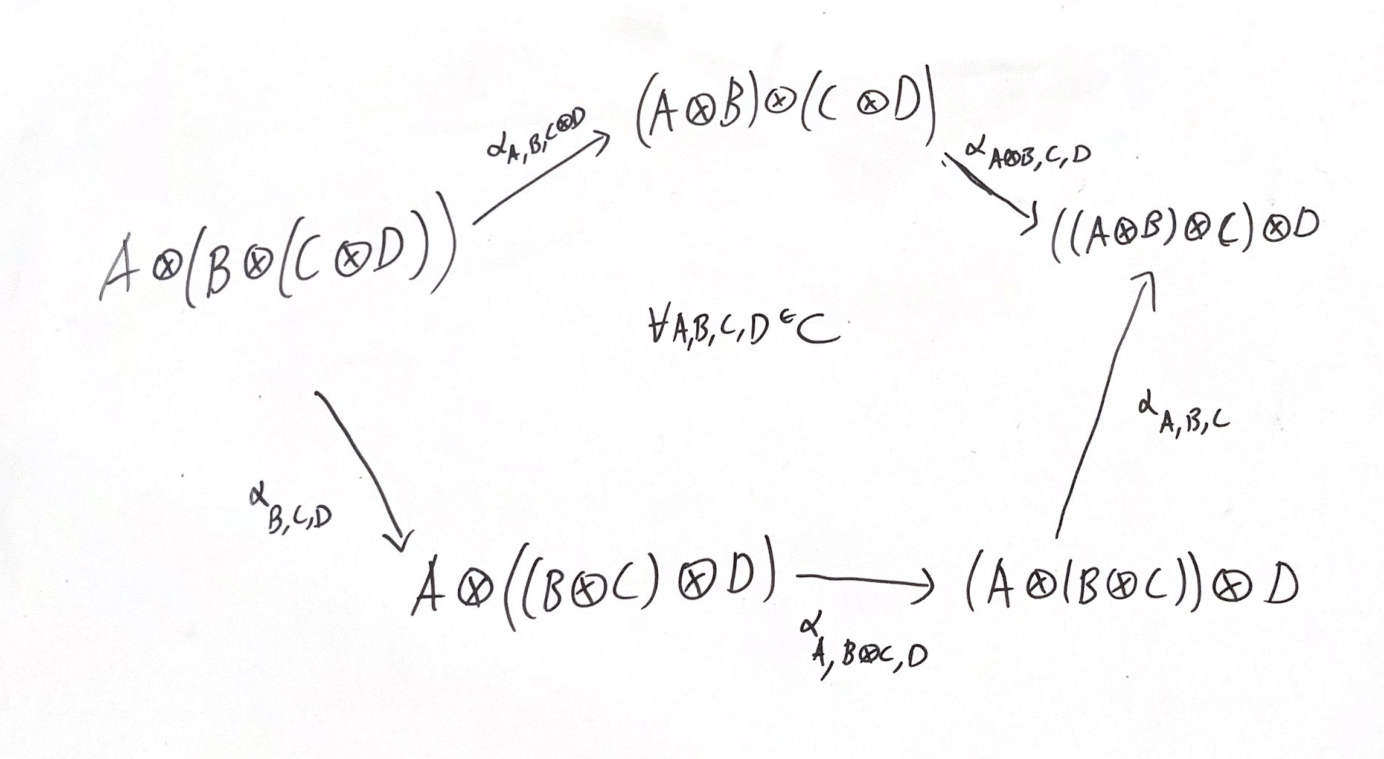
\includegraphics[width=0.7\textwidth]{pent diag.png}
	\caption{Commutative Pentagon Diagram for Monoidal Categories}
\end{figure}


In the context of any nontrivial anyonic system, we intrepret the bifunctor applied to two objects (or tensor product) as being a fusion of two anyons. The identity object represents a trivial fusion. That is, when fusing any particle with the identity, it is equivalent to think that no fusion is happening at all, since the statistic of the fused anyon will not change with respect to the non-identity anyon. The natural isomorphisms reflect physical assertions we make about fusions between the identity and non-identity anyon types. While it is tempting to think that the objects in the category represent the anyons themselves, they actually represent distinct anyon types. More specifically, an anyon's type is distinguished by its statistics. So, viewing anyonic systems through this lens allows us to make conclusions about all anyons who obeys statistics perscribed by their objects. For more information on the explict link between monoidal category theory and boarder physical systems, see \cite{Rose3}

In order to aptly set up our discussion of Fibonacci anyons, we need to further specify our monoidial category. First, we let the objects of this category be the set $\{e,\tau\}$. Then we explicitly define our bifunctor to have the following form:

\begin{equation}
	\begin{aligned}
		\tau \otimes \tau = 1\oplus \tau
	\end{aligned}
\end{equation}

Anyons of type $\tau$ are specifically referred to as the Fibonacci anyons. Our interpretation for the above equation is inherently physical. When Fibonacci anyons fuse together, the resulting quasiparticle does not necessarily obey the same statistics. In our category, there are only two types of anyons, meaning that the fusion of two $\tau$ anyons will yield an anyon of type $e$ or type $\tau$. The direct sum is a probabilistic quantum superposition of states, where each state is represented by the statistics that anyons obey. In this sense, there is some likelihood that the fusion of two Fibonacci anyons will yield another Fibonacci anyon or the fusion will degrade into the vacuum state (we say in this case that the Fibonacci anyons are their own antiparticles). We refer to each outcome as a multi-fushion channel.

In general, we have multiple anyons to keep track of, and the fusion rules ascribed to the system play out in successive fusions of neighboring quasiparticles. If we have $n$ Fibonacci anyons and we track their statistics through their fusion channels, it is no surprise that for any resulting anyon type, the process of arriving to it was not unique. We represent each possible scenario with a diagram, known as a fushion path.

\begin{example}\end{example} 
Suppose we have three Fibonacci anyons. We can illustrate the following fusion paths to see every possible way we can fuse these anyons.

\begin{figure}[H]
	\centering
	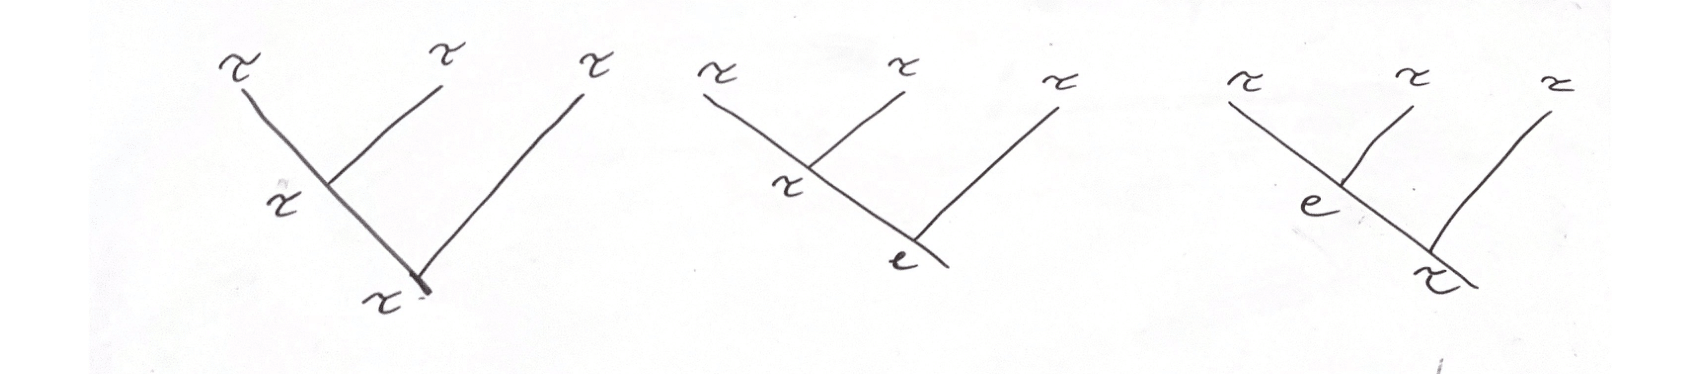
\includegraphics[width=0.7\textwidth]{treebasis.png}
	\caption{These tree diagrams are labelled according to the fusions rules of Fibonacci anyons.}
\end{figure}


These diagrams represent different states of the same anyonic system. If the resulting anyon type is $\tau$, we refer to the fusion tree as representing a ground state. We can use the fusion trees to characterize all possible ground states (degeneracy), and therefore, these trees represent an orthonormal basis of the ground-state manifold\cite{Trebst}. We refer to this as the fusion tree basis of the anyonic system. We can then utilize a combinatorial technique to count the number of ground states (given a fixed number of anyons). If we have $n$ anyons, and $F_n$ represents the number of ground states, we can see that last fusion must have been one of two possible fusions: $\tau\otimes \tau$ or $e \otimes \tau$. In the former scenario, the number of ways for this to happen is characterized by $F_{n-1}$ and in the latter scenario, the number of ways for this to happen is $F_{n-2}$. In general, we can see that the degeneracy of the ground states is exactly equal to the $n^{th}$ Fibonacci number.

Thus far, we have implictly considered fusions to occur successively as outlined by our fusion tree basis. However, in a physical scenario, there is nothing stopping anyons from fusing in a different order. We can use our pentagon diagram above to guide our intuition into how we swap between fusion trees.

Since both fusion trees represent orthonormal bases of the same ground state, they msut be related by a unitary transformation. We call such a transformation an $F$-move. $F$-moves take on the form of matrices whose entries can be specified by a system of equations that generalizes for any $n$ anyon systems. These equations are referred to as the pentagons and they are desugned to explicitly make use of the commutative diagram of the category we are working in. It is worth noting that for each application of an $F$-move, we only alter a component of the fushion tree, not the entire tree. Specifically, we view $F$ matrices as being defined on four anyons: three anyons that will be fused in the tree and one that will be the final result. The $F$ matrix denoted $F^{abc}_d$ defines an $F$ move that exchanges the order of fusion from $(a\otimes b)\otimes c$ to $a\otimes(b\otimes c)$ as depected below.

\begin{figure}[H]
	\centering
	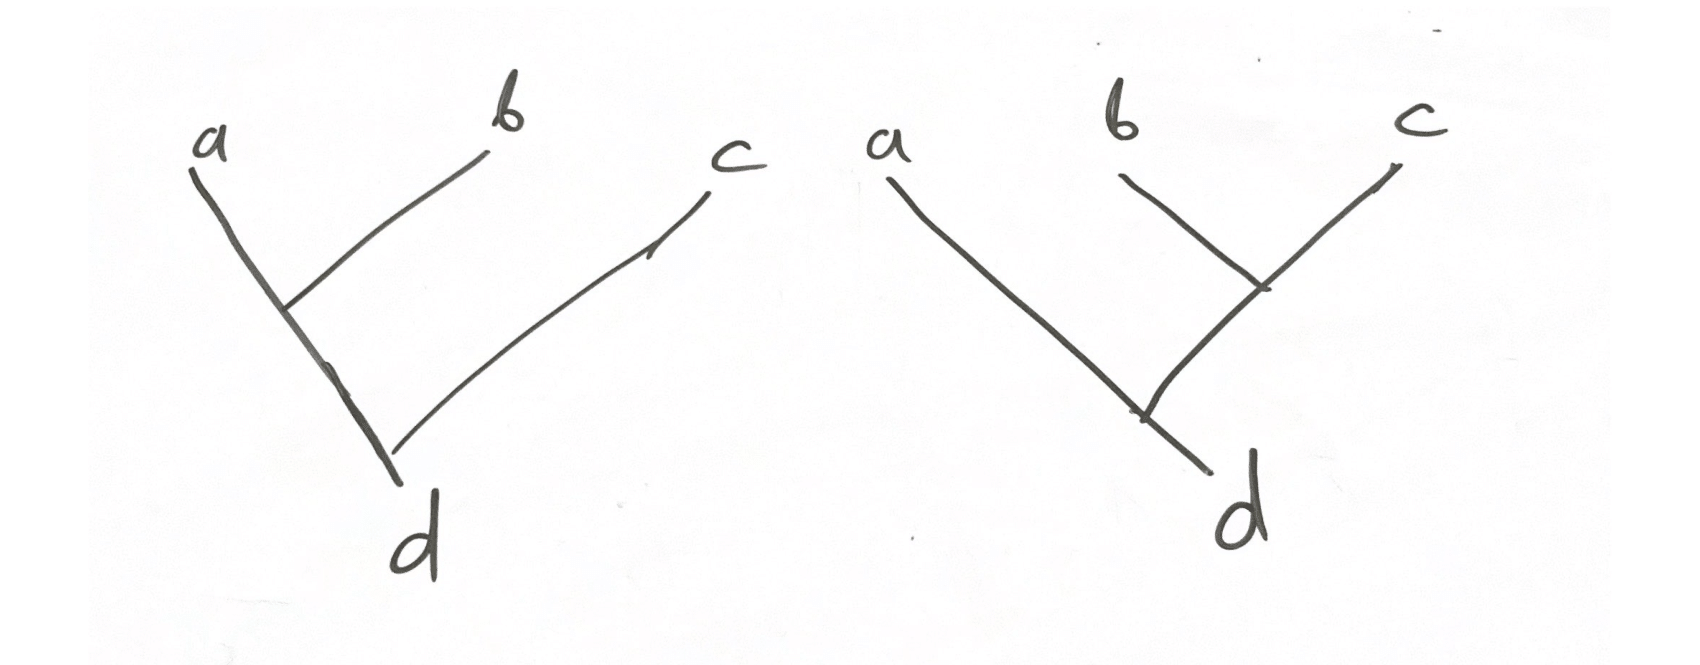
\includegraphics[width=0.7\textwidth]{differentftb}
	\caption{Both tree diagrams represent a different fusion order on the same anyon types.}
\end{figure}

In this sense, we can intuitivley decompose each tree basis into components affected by $F$-moves and components that are not. If we think of each fushion tree as being comprised of two sub-trees joined by one edge, this decomposition is straight forward: For each type of anyon ($e$ and $\tau$), the fusion tree basis for each subtrees (on fewer quasiparticles) can be discerned and then written as a tensor product (corresponding to the whole tree). We take the direct sum of both tensors (one for $e$ and one for $\tau$) to reflect all possible scenarios.

In general, solving for the pentagons is actually quite difficult. But through the study of Fibonacci anyons, we can make some simplifications to our set up. If any anyon is the identity type, our resulting matrix must be the identity matrix (since fusion with this does not impact the overall system). To this end, we need only solve for the transformation matrix when all particles involved are of type $\tau$. The general pentagon equation is written

\begin{equation}
	\begin{aligned}
		[F^{\tau\tau c}_\tau]_{da}[F^{a\tau\tau}_\tau]_{cb} = [F^{\tau\tau \tau}_d]_{cf}[F^{\tau f\tau}_\tau]_{db}[F^{\tau\tau\tau}_b]_{fa}\cite{Trebst}
	\end{aligned}
\end{equation}
where $a,b,c,d,f\in\{e,\tau\}$. Note that the matrices indices are tracked by noninteger values, however the meaning of the subscript is identifies $e$ with the first row/column and $\tau$ with the second row/column. Using the simplfications discussed in the previous paragraph, we can set $b=c=e$ and $a=d=f=\tau$ in order to reduce our equation to 

\begin{equation}
	\begin{aligned}
		[F^{\tau\tau\tau}_\tau]_{11} = [F^{\tau\tau\tau}_\tau]_{12}[F^{\tau\tau\tau}_\tau]_{21}
	\end{aligned}
\end{equation}

where we switch the matrix indices for their integer values for ease of interpretation. Since this transformation is unitary (and based on the number of anyon types, $2\times 2$), we conclude that this matrix must have the following form:

\begin{equation}
	\begin{aligned}
		F^{\tau\tau\tau}_\tau = \begin{bmatrix}
									\frac{1}{\Phi} & \frac{1}{\sqrt{\Phi}}\\
									\frac{1}{\sqrt{\Phi}} & -\frac{1}{\Phi}
								\end{bmatrix}
	\end{aligned}
\end{equation}

where $\Phi$ is the golden ratio.

Now that we have established ways to characterize fusions of anyons, we can intermix discussion of braidings. If we consider a particle exchange of two anyons in an anyonic system, we can expect that the ground state resulting from the fusion of all anyons in the system may be impacted. As such, we can view these transformations in the same context as our $F$-matrices. When two anyons braid, we have a unitary transformation acting on our orthonormal basis of our ground states. Therefore, we can view this transformation in the context of matrix multiplication, and we refer to these anyon braiding matrices as $R$-matrices. We will show that we can obtain a representation of the braid group through combining $F$-matrices and $R$-matrices in a meaningful way. When we incorporate braiding into our problem, we can rigorously define the operation in the concept of a new category.


\begin{definition}
	A \textbf{braided monoidal category} is a monoidal category equipped with a "braiding," $\beta$, which is an isomorphism that satisfies the following commutative diagram:
\end{definition}

\begin{figure}[H]
	\centering
	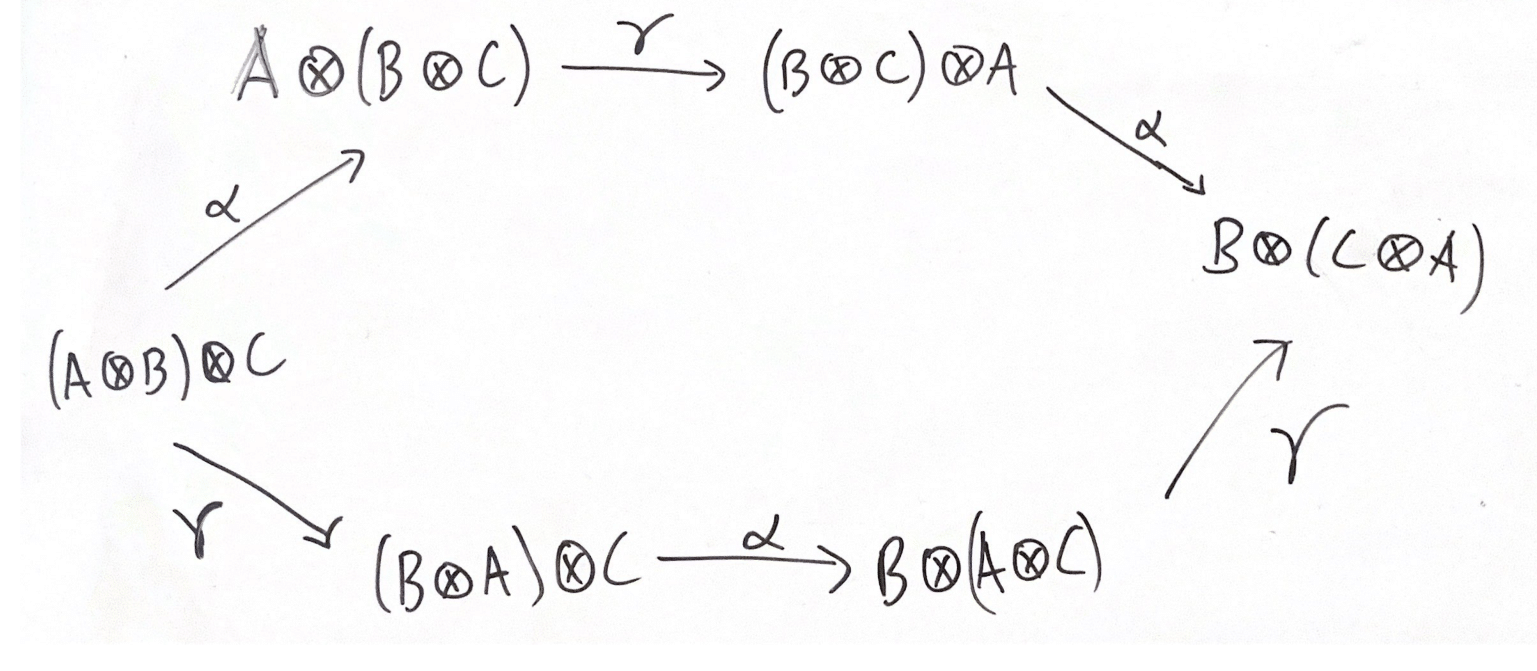
\includegraphics[width=0.7\textwidth]{hexdiag}
	\caption{Hexagonal Commutative Diagram for Braiding Monoidal Categories}
\end{figure}

where $\alpha$ is the associator of the category. For more details on the general properties, see \cite{Joyal}. One idea worth emphasizing here is that in these categories, braiding and fusion are compatible with one another. The best way to think about this is much like the Reidmeister rules from earlier. We can treat tree diagrams as embeddings in three dimensional space, an manipulate the diagram in ways that preserve their structure (isotopy). We can pull fusions under or over braids in the following way:

\begin{figure}[H]
	\centering
	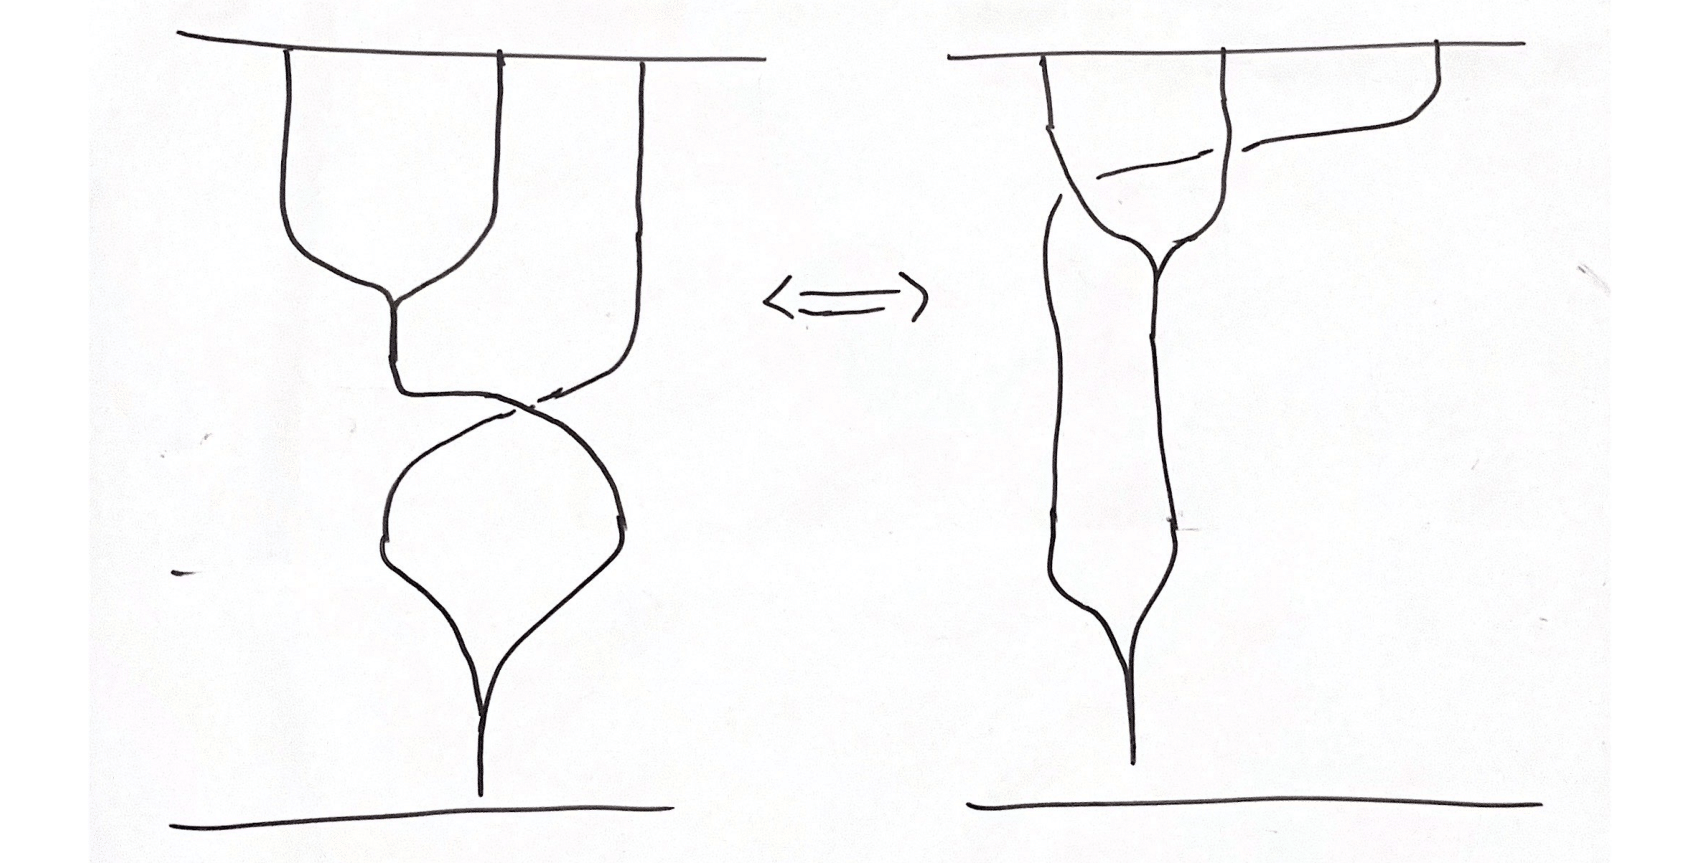
\includegraphics[width=0.7\textwidth]{fusethrubraid.png}
	\caption{Compatibility of braiding and fusion.}
\end{figure}

%As we have seen in our prior discussion of representations of braids defined on the space of wave functions, we can view the action of $R$-matrices not just on our fusion tree basis but the concrete vector space of ground states. That is, since $R$-moves change tree bases, the $R$-matrices must transform orthonormal basis vectors corresponding to them in an identical way. In general, these spaces have a larger dimension than one, and we have nontrivial linear combinations. 

These $R$-matrices can be solved for by utilizing the relations specified in the commutative diagram of the category. If we label $R^{a,b}_c$ as the $R$-matrix who braids the anyons labeled by $a$ and $b$ with total charge $c$, then the following system of equations are referred to as the hexagons:

\begin{equation}
	\begin{aligned}
		R^{\tau,\tau}_c [F^{\tau\tau\tau}_\tau]_{ca}R^{\tau,\tau}_a = \sum_b [F^{\tau\tau\tau}_\tau]_{cb}R^{\tau,b}_\tau[F^{\tau\tau\tau}_\tau]_{ba} \cite{Trebst}
	\end{aligned}
\end{equation}

where $a,b,c\in\{e,\tau\}$ and we again reference the matrix entries based on the row/column values perscribed to $e$ and $\tau$ above. We also note that braiding any $e$ anyon around a $\tau$ anyon leads to no change, and should mean the $R$-matrices would be the identity matrix. Therefore, we get a complicated system of equations.

\begin{equation}
	\begin{aligned}
		(R^{\tau,\tau}_e)^2\frac{1}{\Phi} = R^{\tau,\tau}_\tau\frac{1}{\Phi} + \frac{1}{\Phi^2}
	\end{aligned}
\end{equation}
\begin{equation}
	\begin{aligned}
		R^{\tau,\tau}_eR^{\tau,\tau}_\tau\frac{1}{\sqrt{\Phi}} = (1-R^{\tau,\tau}_\tau)\frac{1}{\Phi^\frac{3}{2}} 
	\end{aligned}
\end{equation}
\begin{equation}
	\begin{aligned}
		-(R^{\tau,\tau}_e)^2\frac{1}{\Phi} = R^{\tau,\tau}_\tau\frac{1}{\Phi^2}+\frac{1}{\Phi}
	\end{aligned}
\end{equation}

If we take our state space to be one dimensional, the $R$-matrices are complex numbers, and we can characterize them much more easily with the solutions $R^{\tau\tau}_e = e^{i\frac{4\pi}{5}}$ and $R^{\tau\tau}_\tau = e^{i\frac{-3\pi}{5}}$. The general braid representation matrices take the form of 

\begin{equation}
	\begin{aligned}
		B = F^{-1}R F
	\end{aligned}
\end{equation}

where we interpret our $F$ matrices as change of basis transformation on the underlying state space and $R$ represents an exchange of two anyons. A more geometrical interpretation for this action is to take two anyons, denoted by the type $\tau$, to fuse them together, then interchange them, and then to unfuse them (preserving the interchange). 

\begin{figure}[H]
	\centering
	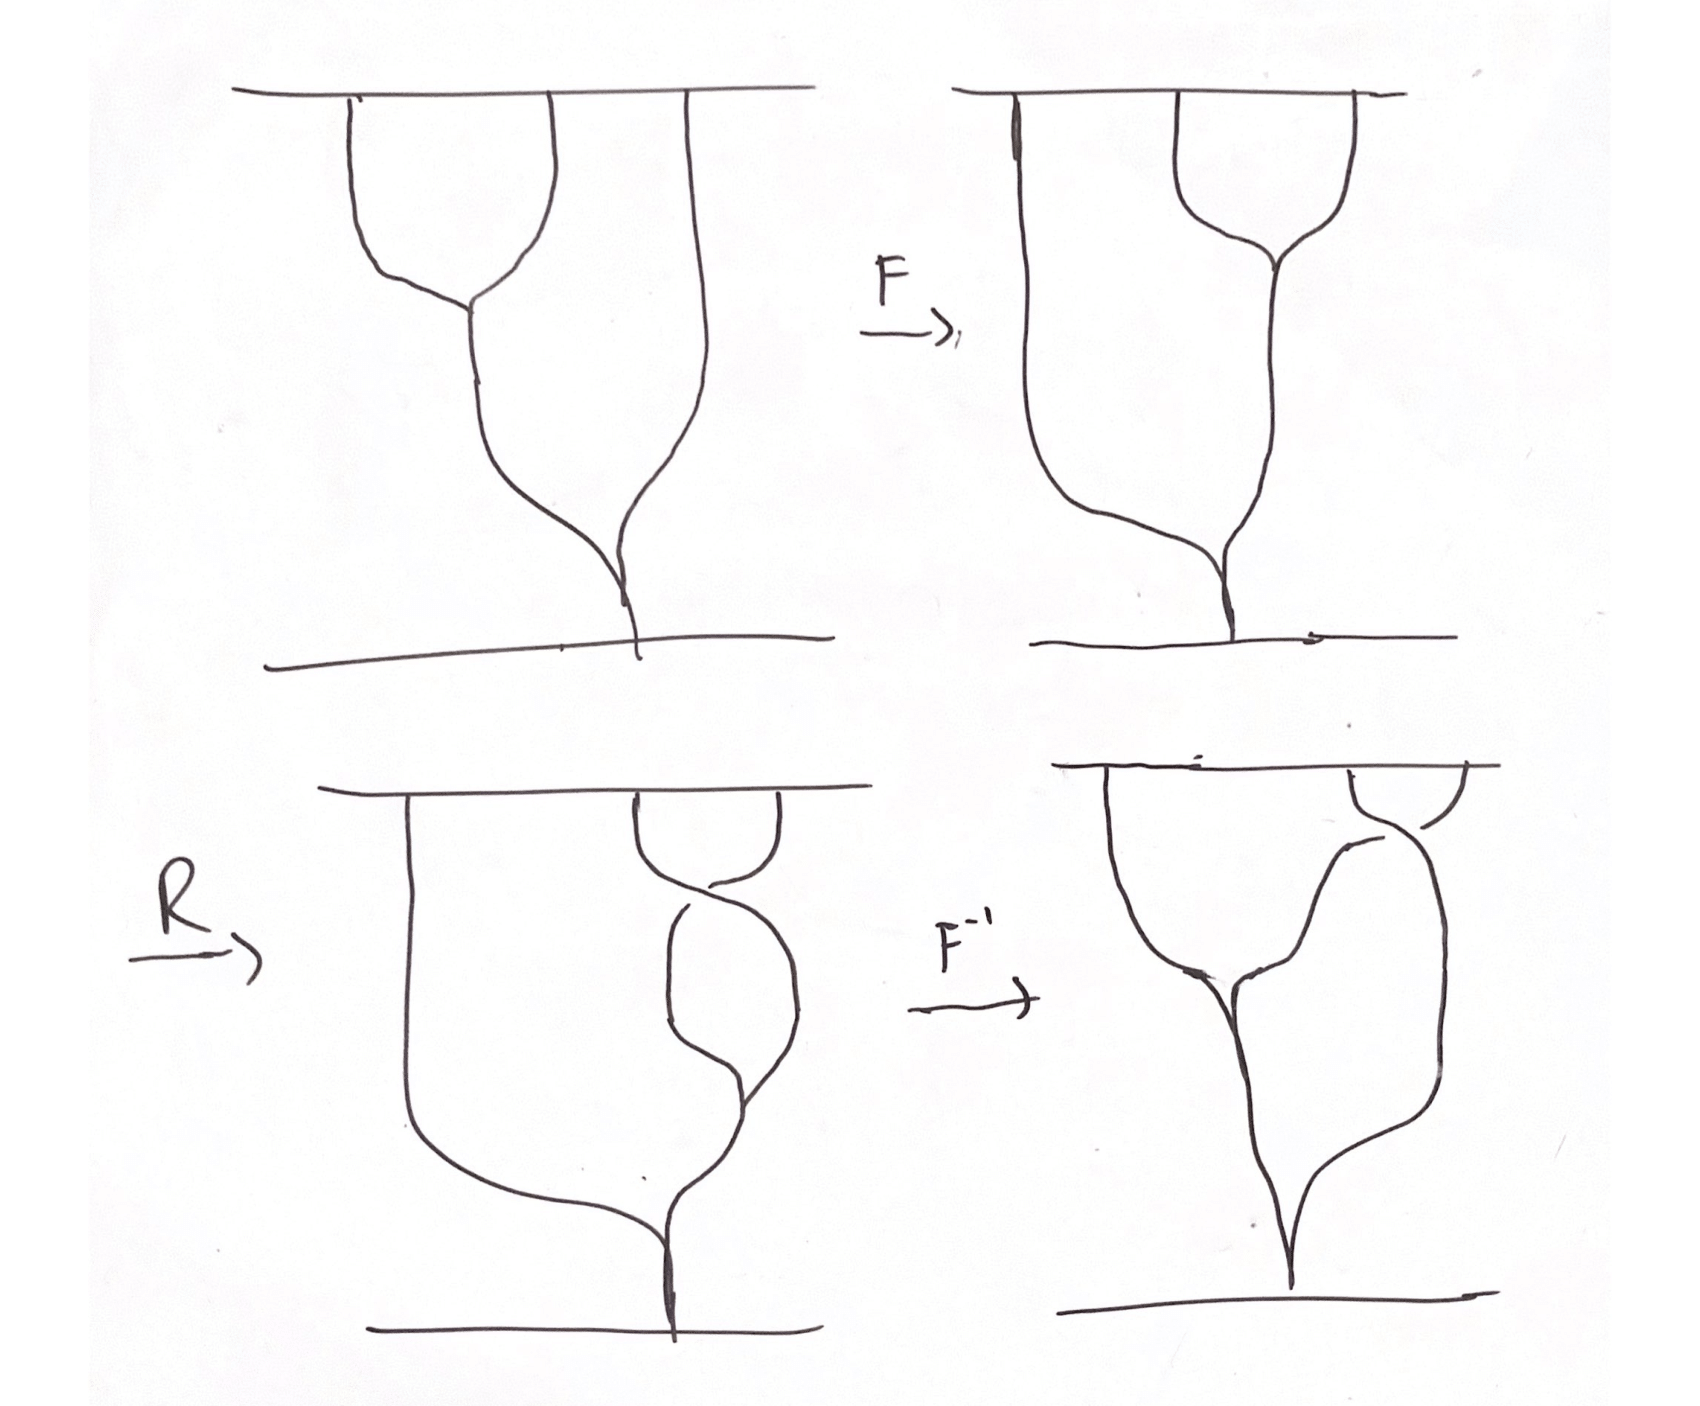
\includegraphics[width=0.7\textwidth]{braid.png}
	\caption{The process of braiding decomposed into fusion and anyon exchanges.}
\end{figure}

At this point, it should be noted that without more specificity it is quite difficult to explicitly compute these matrices. We will use a simple example to illustrate what the general approach would be.

\begin{example}
\end{example}
Suppose that we have two adjacent $\tau$ anyons whose collective charge is $\tau$ after being fused. We label the intermediately fused anyons as by the markers $a,b,c$ successively, we can identify five valid choices: $\{e\tau e,\tau\tau e, e\tau\tau, \tau e\tau, \tau\tau\tau\}$. These states will form the basis of our vector space.

\begin{figure}[H]
	\centering
	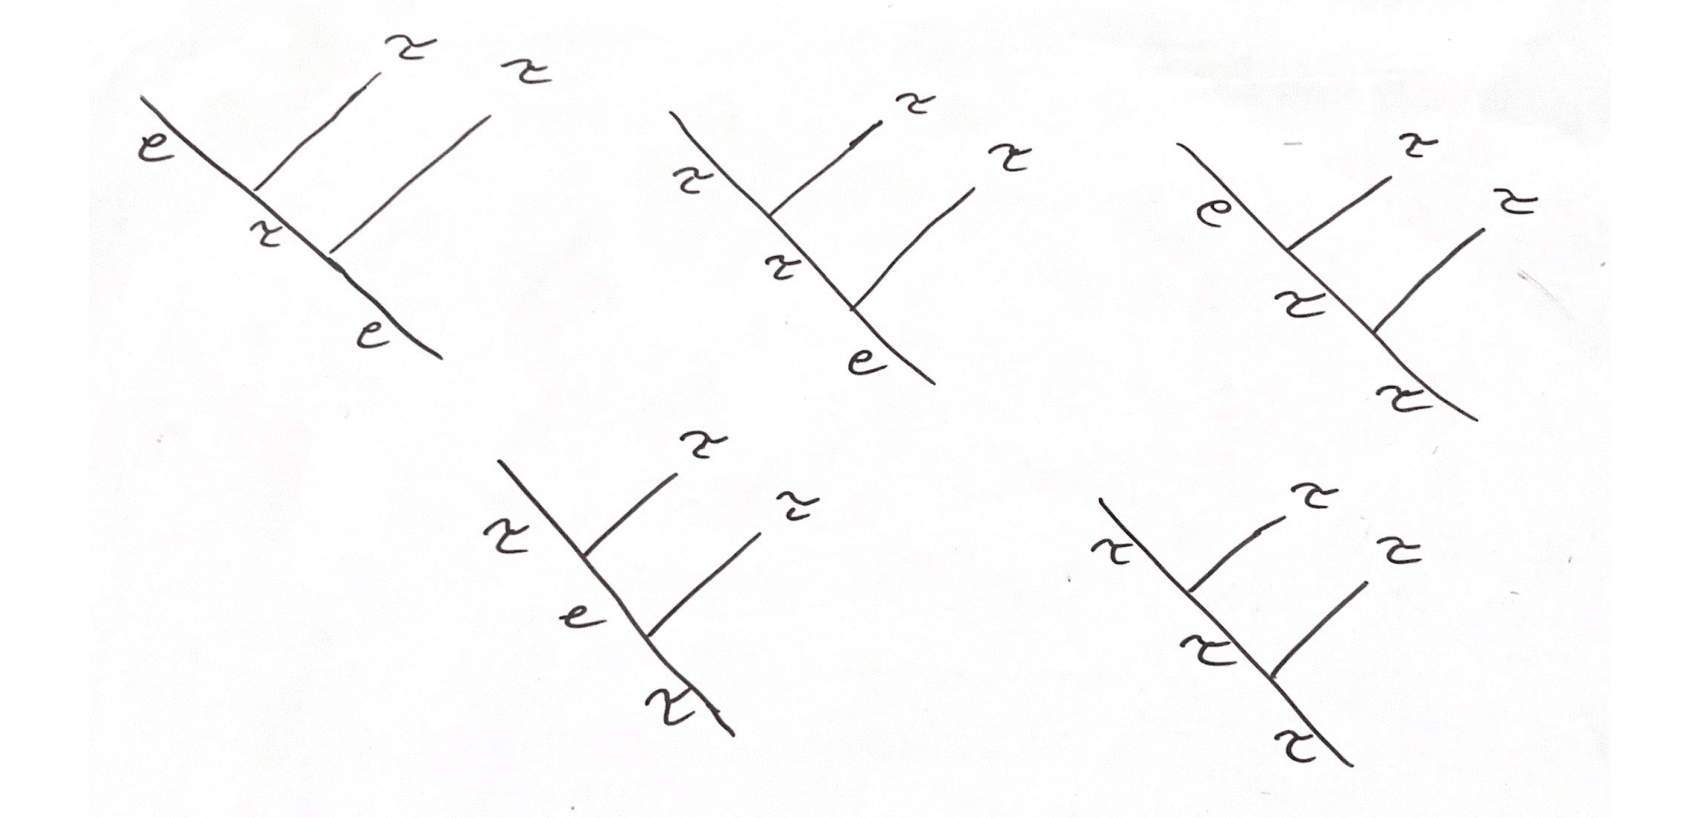
\includegraphics[width=0.7\textwidth]{fivetrees.png}
	\caption{These five trees represent all valid choices for labeling intermediate fusions.}
\end{figure}

If we use the $F$-move that fuses our anyons together, we end up with a new choice of the intermediate fusions: $\{e\tau e,\tau\tau e, e\tau\tau, \tau e\tau, \tau\tau\tau\}$. This transformation is represented by the following $F$-matrix:

\begin{equation}
	\begin{aligned}
		F = \begin{bmatrix}
				1 & 0 & 0 & 0 & 0 \\
				0 & 1 & 0 & 0 & 0 \\
				0 & 0 & 1 & 0 & 0 \\
				0 & 0 & 0 & \frac{1}{\Phi} & \frac{1}{\sqrt{\Phi}}\\
				0 & 0 & 0 &\frac{1}{\sqrt{\Phi}} & -\frac{1}{\Phi}
			\end{bmatrix}\cite{Trebst}
	\end{aligned}
\end{equation}

with respect to the basis of states described. By identifying the $R$-move necessary to exchange the anyons given its state, we see that our $R$-matrix takes the following form:

\begin{equation}
	\begin{aligned}
		R = \begin{bmatrix}
				e^{i\frac{4\pi}{5}} & 0 & 0 & 0 & 0 \\
				0 & e^{i\frac{-3\pi}{5}} & 0 & 0 & 0 \\
				0 & 0 & e^{i\frac{-3\pi}{5}} & 0 & 0 \\
				0 & 0 & 0 & e^{i\frac{4\pi}{5}} & 0\\
				0 & 0 & 0 & 0 &e^{i\frac{-3\pi}{5}} 
			\end{bmatrix}
	\end{aligned}
\end{equation}

Therefore, we can construct the braid matrix

\begin{equation}
	\begin{aligned}
		B = \begin{bmatrix}
				e^{i\frac{4\pi}{5}} & 0 & 0 & 0 & 0 \\
				0 & e^{i\frac{-3\pi}{5}} & 0 & 0 & 0 \\
				0 & 0 & e^{i\frac{-3\pi}{5}} & 0 & 0 \\
				0 & 0 & 0 & \frac{-e^{i\frac{4\pi}{5}}}{\Phi^2} + \frac{-e^{i\frac{-3\pi}{5}}}{\Phi}& \frac{-e^{i\frac{4\pi}{5}}}{\Phi^\frac{3}{2}} + \frac{e^{i\frac{-3\pi}{5}}}{\Phi^\frac{3}{2}}\\
				0 & 0 & 0&\frac{-e^{i\frac{4\pi}{5}}}{\Phi^\frac{3}{2}} + \frac{e^{i\frac{-3\pi}{5}}}{\Phi^\frac{3}{2}} &\frac{-e^{i\frac{4\pi}{5}}}{\Phi^2} + \frac{-e^{i\frac{-3\pi}{5}}}{\Phi}
			\end{bmatrix}
	\end{aligned}
\end{equation}

This matrix characterizes the behavior of two Fibonacci anyons braiding with one another given the ground states of our two anyons are all one dimensional. If we were to look at all the anyons in our system, we would see more complicated matrices take form. Most easily, we could generalize these interactions to more anyons in the system if we were to consider more fusions and exchanges happening successively. Such a braid matrix would take the following form

\begin{equation}
	\begin{aligned}
		B = \prod_i F_i^{-1}R_iF_i
	\end{aligned}
\end{equation}

where each factor in the product represents a single exchange of two specified anyons specified by the choice of $F_i$ and $R_i$. It is not unreasonable to see that given more specification on our space we could construct a representation using matrices of these form.
\chapter{Conclusion}
As we have seen, representation theory pulls insight from a diverse set of mathematical disciplines to create meaningful techniques to interpret even the most complicated groups. The representations we calculated in this thesis hold important physical significance. While we have only explored the representations of a handful of groups, representation theory can be used to characterize the behavior of many different physical systems. To briefly touch on a few, the Heisenberg group, the special unitary group, and the Galilean group can be analyzed in the by examining the physical symmetries that are inherent to their structure. Further, the study of representations of $C^*$-algebras, quantum groups, and Kac-Moody algebras are particularly relevant to theoretical physics in the realm of quantum field theory and exactly solvable models. Finally, generalizations of representation theory to categories give us surprisingly useful insight into the inner workings of physical systems. 

It is clear there is no shortage of avenues to explore the study of representation theory. While the further development of the mathematics and the physics required to explore more of this subject is nontrivial, the path illustrated gives rise to many opportunities to learn new methods to characterize the mathematical structure underpinning physical phenomena. Representations of these groups provide insight into the complex systems that govern our world.




\bibliographystyle{abbrv}
\bibliography{ref}




\end{document}